%%%%%%%%%%%%%%%%%%%%%%%%%%%%%%%%%%%%%%%%%%%%%%%%%%%%%%%%%%%%%%%%%%%%%
%
% Complete documentation on the extended LaTeX markup used for Insight
% documentation is available in ``Documenting Insight'', that is part
% of the standard documentation for Insight.  It may be found online
% at:
%
%                    http://www.itk.org
%
%%%%%%%%%%%%%%%%%%%%%%%%%%%%%%%%%%%%%%%%%%%%%%%%%%%%%%%%%%%%%%%%%%%%%

\documentclass{InsightSoftwareGuide}

\usepackage[dvips]{graphicx}
\usepackage{times}
\usepackage{xcolor}
\usepackage{listings}
\usepackage{minted}
\usepackage{setspace}
\usepackage{hyphenat}
\usepackage[toc,page]{appendix}
\usepackage{verbatim}
\usepackage{imakeidx}
%\usepackage{siunitx}
\usepackage[papersize={7.5in,9.25in},margin=1in]{geometry}

%%%%%%%%%%%%%%%%%%%%%%%%%%%%%%%%%%%%%%%%%%%%%%%%%%%%%%%%%%%%%%%%%%%
%
%
%   Load configuration parameters prepared by CMake
%
%
%%%%%%%%%%%%%%%%%%%%%%%%%%%%%%%%%%%%%%%%%%%%%%%%%%%%%%%%%%%%%%%%%%%
\input{SoftwareGuideConfiguration.tex}


\ifitkDraftWatermark
\usepackage{draftwatermark}
\SetWatermarkText{DRAFT-ITK}%default is DRAFT
\SetWatermarkLightness{0.90}%default is 0.8
\SetWatermarkScale{0.8}%default is 1.2
\fi

%\allowhyphens

\lstnewenvironment{itklisting}
{\singlespacing\lstset{language=C++}}
{}

\definecolor{ltgray}{rgb}{0.93,0.93,0.93}
\usemintedstyle{emacs}

\lstset{
         basicstyle=\footnotesize\ttfamily, % Default font
         %numbers=left,               % The size of the fonts that are used for the code
         numberstyle=\tiny,           % The style that is used for the line-numbers
         %stepnumber=2,               % The step between two line-numbers. If it's 1, each line will be numbered
         numbersep=2pt,               % How far the line-numbers are from the code
         tabsize=2,                   % Sets default tabsize to 2 spaces
         extendedchars=true,          % Lets you use non-ASCII characters; for 8-bits encodings only, does not work with UTF-8
         breaklines=true,             % Sets automatic line breaking
         keywordstyle=\color{red},
 %    frame=b,
 %        keywordstyle=[1]\textbf,    % Keyword style
 %        keywordstyle=[2]\textbf,    %
 %        keywordstyle=[3]\textbf,    %
 %        keywordstyle=[4]\textbf,   \sqrt{\sqrt{}} %
         stringstyle=\color{black}\ttfamily, % Style of string literals
         showspaces=false,           % Show spaces everywhere adding particular underscores; it overrides 'showstringspaces'
         showtabs=false,             % Show tabs within strings adding particular underscores
         xleftmargin=17pt,
         framexleftmargin=17pt,
         framexrightmargin=5pt,
         framexbottommargin=4pt,
         backgroundcolor=\color{ltgray}, % Choose the background color; you must add \usepackage{color} or \usepackage{xcolor}
         showstringspaces=false      % Underline spaces within strings only
 }

 \lstloadlanguages{% Check Documentation for further languages ...
         %[Visual]Basic
         %Pascal
         %C
         C++
         %XML
         %HTML
         %Java
 }
%\DeclareCaptionFont{blue}{\color{blue}}

%\captionsetup[lstlisting]{singlelinecheck=false, labelfont={blue}, textfont={blue}}
\usepackage{caption}
\DeclareCaptionFont{white}{\color{white}}
\DeclareCaptionFormat{listing}{\colorbox[cmyk]{0.43, 0.35, 0.35,0.01}{\parbox{\textwidth}{\hspace{15pt}#1#2#3}}}
\captionsetup[lstlisting]{format=listing,labelfont=white,textfont=white, singlelinecheck=false, margin=0pt, font={bf,footnotesize}}


%%%%%%%%%%%%%%%%%%%%%%%%%%%%%%%%%%%%%%%%%%%%%%%%%%%%%%%%%%%%%%%%%%
%
%  hyperref should be the last package to be loaded.
%
%%%%%%%%%%%%%%%%%%%%%%%%%%%%%%%%%%%%%%%%%%%%%%%%%%%%%%%%%%%%%%%%%%
\ifitkPrintedVersion
\usepackage[dvips,
pdftitle={ITK Software Guide},
pdfauthor={Hans Johnson and Luis Ib'{a}~{n}ez and Matthew McCormick and the Insight Software Consortium},
pdfsubject={Medical Image Segmentation and Registration Toolkit}
pdfkeywords={Registration,Segmentation,Guide},
pdfpagemode={UseOutlines},
bookmarks,bookmarksopen,
pdfstartview={FitH},
backref,
colorlinks,linkcolor={black},citecolor={black},urlcolor={black},
]{hyperref}
\else
\usepackage[dvips,
pdftitle={ITK Software Guide},
pdfauthor={Hans Johnson and Luis Ib'{a}~{n}ez and Matthew McCormick and the Insight Software Consortium},
pdfsubject={Medical Image Segmentation and Registration Toolkit},
pdfkeywords={Registration,Segmentation,Guide},
pdfpagemode={UseOutlines},
bookmarks,bookmarksopen,
pdfstartview={FitH},
backref,
colorlinks,linkcolor={blue},citecolor={blue},urlcolor={blue},
]{hyperref}
\fi

%%%%%%%%%%%%%%%%%%%%%%%%%%%%%%%%%%%%%%%%%%%%%%%%%%%%%%%%%%%%%%%%%%%
%
%
%           The Insight Toolkit Software Guide
%
%
%%%%%%%%%%%%%%%%%%%%%%%%%%%%%%%%%%%%%%%%%%%%%%%%%%%%%%%%%%%%%%%%%%%

\author{Hans J. Johnson, Matthew M. McCormick, Luis Ib\'{a}\~{n}ez, and the \emph{Insight Software Consortium}}

\authoraddress{
  \url{https://itk.org}\\
  Email: \email{community@itk.org}
}

\date{\today}

% actually write the .idx file
\makeindex

\setcounter{tocdepth}{3}



\title{The ITK Software Guide\\Book 1: Introduction and Development Guidelines\\Fourth Edition\\ \emph{Updated for ITK version
\ITKVERSIONMAJORMINOR}}


%%%%%%%%%%%%%%%%%%%%%%%%%%%%%%%%%%%%%%%%%%%%%%%%%%%%%%%%%%%%%%%%%%%
%
%           Begin Document
%
%%%%%%%%%%%%%%%%%%%%%%%%%%%%%%%%%%%%%%%%%%%%%%%%%%%%%%%%%%%%%%%%%%%

\begin{document}

\ifitkPrintedVersion

  \begin{minipage}[t][3cm][b]{\textwidth}
  \rule{14cm}{1pt}
  \end{minipage}

  \begin{minipage}[t][3cm][b]{\textwidth}
  \Huge
  The ITK Software Guide\\
  Book 1: Introduction and Development Guidelines\\
  \normalsize
  \par
  \emph{Updated for version \ITKVERSIONMAJORMINOR}\\

  \end{minipage}

  \hfill
\begin{minipage}[t][6cm][b]{0.6\textwidth}
\Large
\renewcommand{\baselinestretch}{1.5}
Hans J. Johnson\\
Matt McCormick \\
Luis Ib\'{a}\~{n}ez\\
and the \emph{Insight Software Consortium}
\normalsize
\end{minipage}


\begin{minipage}[t][2cm][b]{\textwidth}
\rule{14cm}{1pt}
\end{minipage}

\newpage

\begin{minipage}[t][4cm][b]{\textwidth}
\begin{center}

\includegraphics[width=0.5\textwidth]{Kitware-logo-medium-res.eps}
\end{center}
\par
\begin{center}
\large

\copyright \the\year Kitware, Inc. \emph{(cover, preface, postface)}\\
\copyright \the\year Insight Software Consortium \emph{(main text body)}\\
Published by Kitware, Inc. \texttt{http://www.kitware.com}
\normalsize
\end{center}
\end{minipage}


\begin{minipage}[t][2.25cm][b]{\textwidth}
\begin{center}
An electronic version of this document is available from
\texttt{http://www.itk.org} and may be used under the provisions of the
ITK copyright found at \texttt{http://www.itk.org/HTML/Copyright.htm}.
\end{center}
\end{minipage}


%\begin{minipage}[t][3.2cm][b]{\textwidth}
%\begin{center}
%The publisher Kitware, Inc. offers discounts on this book when ordered in
%bulk quantities.\\
%The publisher also produces companion works to this text such as \emph{The
%Visualization Toolkit An Object-Oriented Approach to 3D Graphics 3rd Edition}
%by Schroeder, Martin and Lorensen, \emph{Mastering CMake} by Martin and
%Hoffman and \emph{The VTK's Users Guide} by Kitware.\\
%For more information contact Kitware, Inc at \texttt{kitware@kitware.com}.\\
%You may also order directly from Kitware's electronic store at
%\texttt{http://www.kitware.com/products}\\
%\end{center}
%\end{minipage}


\begin{minipage}[t][2.5cm][b]{\textwidth}
\begin{center}
This project has been funded in whole or in part with Federal funds from the
National Institutes of Health (NLM, NIDCR, NIMH, NEI, NINDS, NIDCD, NCI), the
NSF, and the DoD (TATRC) under the direction of the National Library of
Medicine, National Institutes of Health, contracts number N01-LM-9-3531,
N01-LM-9-3532, N01-LM-0-3501, N01-LM-0-3502, N01-LM-0-3503, and
N01-LM-0-3504.  \bf{TODO:  Terry Yoo to provide more information}
\end{center}
\end{minipage}


\begin{minipage}[t][1.0cm][b]{\textwidth}
\begin{center}
All product names mentioned herein are the trademarks of their respective
owners.
\end{center}
\end{minipage}

  \begin{minipage}[t][1.0cm][b]{\textwidth}
\begin{center}
Printed and produced in the United States of America.\\
\bf{ISBN 9781-930934-28-3}
\end{center}
\end{minipage}


\fi

\maketitle

\frontmatter

\hyperbaseurl{http://www.itk.org/Insight}


%%%%%%%%%%%%%%%%%%%%%%%%%%%%%%%%%%%%%%%%%%
%
%  Page with Quote and ITK Logo
%
%
%%%%%%%%%%%%%%%%%%%%%%%%%%%%%%%%%%%%%%%%%%
\cleardoublepage

\begin{minipage}[t][10cm][b]{\textwidth}
\center

\includegraphics[width=0.5\textwidth]{itkLogo.eps}
\large
\begin{center}
\emph{The purpose of computing is Insight, not numbers.}\\
\end{center}
\hspace{8cm} Richard Hamming
\normalsize
\end{minipage}



%%%%%%%%%%%%%%%%%%%%%%%%%%%%%%%%%%%%%%%%%%%%%%
%
% remove headings from the following material
\pagestyle{plain}
%
%%%%%%%%%%%%%%%%%%%%%%%%%%%%%%%%%%%%%%%%%%%%%%


\ifitkPrintedVersion
  % We want this material to fit on two pages
\small

\chapter*{About the Cover}

Creating the cover image demonstrating the capabilities of the toolkit was a
challenging task.\footnote{The source code for the cover is available from
SoftwareGuide/Cover/Source/ directory of the ITKSoftwareGuide repository.}
Given that the origins of ITK are with the Visible Human Project, it was
decided to create the cover image from the Visible Woman dataset, which is one
of the more recently acquired datasets of the Visible Human Project.  Both the
RGB cryosections and the CT scans were combined in the same scene.

\begin{description}

\item [Removing the Gel.]
The body of the Visible Woman was immersed in a block of gel during the
freezing process. This gel appears as a blue material in the cryogenic data.
To remove the gel, the joint histogram of RGB values was computed. This
resulted in an 3D image of $256\times256\times256$ pixels. The histogram
image was visualized in VolView.\footnote{VolView is a commercial product
from Kitware. It supports ITK plug-ins and is available as a free viewer or
may be licensed with advanced functionality. See
http://www.kitware.com/products/volview.html for information.} The cluster
corresponding to the statistical distribution of blue values was identified
visually, and a separating plane was manually defined in RGB space. The
equation of this plane was subsequently used to discriminate pixels in the
gel from pixels in the anatomical structures. The gel pixels were zeroed out
and the RGB values on the body were preserved.

\item[The Skin.]
The skin was easy to segment once the gel was removed. A simple region
growing algorithm was used requiring seed points in the region previously
occupied by the gel and then set to zero values. An anti-aliasing filter was
applied in order to generate an image of pixel type float where the surface
was represented by the zero set. This dataset was exported to VTK where a
contouring filter was used to extract the surface and introduce it in the VTK
visualization pipeline.

\item[The Brain.]
The visible part of the brain represents the surface of the gray matter.  The
brain was segmented using the vector version of the confidence connected
image filter.  This filter implements a region growing algorithm that starts
from a set of seed points and adds neighboring pixels subject to a condition
of homogeneity.

The set of sparse points obtained from the region growing algorithm was
passed through a mathematical morphology dilation in order to close holes and
then through a binary median filter. The binary median filter has the
outstanding characteristic of being very simple in implementation by applying
a sophisticated effect on the image. Qualitatively it is equivalent to a
curvature flow evolution of the iso-contours. In fact the binary median
filter as implemented in ITK is equivalent to the majority filter that
belongs to the family of voting filters classified as a subset of the
\emph{Larger than Life} cellular automata. Finally, the volume resulting from
the median filter was passed through the anti-aliasing image filter. As
before, VTK was used to extract the surface.

\item[The Neck Musculature.]
The neck musculature was not perfectly segmented. Indeed, the resulting
surface is a fusion of muscles, blood vessels and other anatomical
structures. The segmentation was performed by applying the
VectorConfidenceConnectedImageFilter to the cryogenic dataset. Approximately
60 seed points were manually selected and then passed to the filter as
input. The binary mask produced by the filter was dilated with a mathematical
morphology filter and smoothed with the BinaryMedianImageFilter. The
AntiAliasBinaryImageFilter was used at the end to reduce the pixelization
effects prior to the extraction of the iso-surface with vtkContourFilter.

\item[The Skull.]
The skull was segmented from the CT dataset and registered to the cryogenic
data. The segmentation was performed by simple thresholding, which was good
enough for the cover image. As a result, most of the bone structures are
actually fused together. This includes the jaw bone and the cervical
vertebrae.

\item[The Eye.]
The eye is charged with symbolism in this image. This is due in part because
the motivation for the toolkit is the analysis of the Visible Human data,
and in part because the name of the toolkit is \emph{Insight}.

The first step in processing the eye was to extract a sub-image of
$60\times60\times60$ pixels centered around the eyeball from the RGB
cryogenic dataset. This small volume was then processed with the vector
gradient anisotropic diffusion filter in order to increase the homogeneity of
the pixels in the eyeball.

The smoothed volume was segmented using the
VectorConfidenceConnectedImageFilter using 10 seed points. The resulting
binary mask was dilated with a mathematical morphology filter with a
structuring element of radius one, then smoothed with a binary mean image
filter (equivalent to majority voting cellular automata). Finally the mask
was processed with the AntiAliasBinaryImageFilter in order to generate a
float image with the eyeball contour embedded as a zero set.

\item[Visualization.]
The visualization of the segmentation was done by passing all the binary
masks through the AntiAliasBinaryImageFilter, generating iso-contours with
VTK filters, and then setting up a VTK Tcl script. The skin surface was
clipped using the vtkClipPolyDataFilter using the implicit function
vtkCylinder. The vtkWindowToImageFilter proved to be quite useful for
generating the final high resolution rendering of the scene ($3000\times3000$
pixels).

\item[Cosmetic Postprocessing.]
We have to confess that we used Adobe Photoshop to post-process the image. In
particular, the background of the image was adjusted using Photoshop's color
selection. The overall composition of the image with the cover text and
graphics was also performed using Photoshop.

\end{description}

\normalsize

\fi

\ifitkFullVersion
  \chapter*{Abstract}
\noindent
The National Library of Medicine Insight Segmentation and Registration Toolkit,
shortened as the Insight Toolkit \href{https://itk.org}{(ITK)}, is an
open-source software toolkit for performing registration and
segmentation. \emph{Segmentation} is the process of identifying and
classifying data found in a digitally sampled
representation. Typically the sampled representation is an image
acquired from such medical instrumentation as CT or MRI
scanners. \emph{Registration} is the task of aligning or developing
correspondences between data. For example, in the medical environment,
a CT scan may be aligned with a MRI scan in order to combine the
information contained in both.

ITK is a cross-platform software. It uses a build environment known as
\href{https://cmake.org}{CMake} to manage platform-specific project
generation and compilation process in a platform-independent way. ITK is
implemented in C++. ITK's implementation style employs generic programming,
which involves the use of templates to generate, at compile-time, code that can
be applied \emph{generically} to any class or data-type that supports the
operations used by the template. The use of C++ templating means that the code
is highly efficient and many issues are discovered at compile-time, rather than
at run-time during program execution. It also means that many of ITK's
algorithms can be applied to arbitrary spatial dimensions and pixel types.

An automated wrapping system integrated with ITK generates an interface between
C++ and a high-level programming language \href{http://www.python.org}{Python}.
This enables rapid prototyping and faster exploration of ideas by shortening the
edit-compile-execute cycle. In addition to automated
wrapping, the \href{https://www.itk.org/Wiki/SimpleITK}{SimpleITK} project
provides a streamlined interface to ITK that is available for C++, Python, Java,
CSharp, R, Tcl and Ruby.

Developers from around the world can use, debug, maintain, and extend the
software because ITK is an open-source project. ITK uses a
model of software development known as Extreme
Programming. Extreme Programming collapses the usual software development
methodology into a simultaneous iterative process of
design-implement-test-release. The key features of Extreme Programming
are communication and testing. Communication among the members of the
ITK community is what helps manage the rapid evolution of the
software. Testing is what keeps the software stable. An
extensive testing process supported by the system known as
\href{http://open.cdash.org/index.php?project=Insight}{CDash}
measures the quality of ITK code on a daily basis. The ITK Testing Dashboard is
updated continuously, reflecting the quality of the code at any moment.

The most recent version of this document is available online at
\url{https://itk.org/ItkSoftwareGuide.pdf}.

  This book is a guide to developing software with ITK; it is the first of two
companion books. This book covers building and installation, general
architecture and design, as well as the process of contributing in the ITK
community.  The second book covers detailed design and functionality for
reading and and writing images, filtering, registration, segmentation, and
performing statistical analysis.

  \chapter*{Contributors}
\noindent

The Insight Toolkit \href{http://www.itk.org}{(ITK)} has been created by the
efforts of many talented individuals and prestigious organizations. It is also
due in great part to the vision of the program established by Dr. Terry Yoo
and Dr. Michael Ackerman at the National Library of Medicine.

This book lists a few of these contributors in the following paragraphs. Not
all developers of ITK are credited here, so please visit the Web pages at
\href{http://www.itk.org/HTML/About.htm}{http://www.itk.org/HTML/About.htm} 
for the names of additional contributors, as well as checking the GITS source
logs for code contributions.

The following is a brief description of the contributors to this software
guide and their contributions.


\huge{TO BE DETERMINED FOR ITK 4.4.0 Software Guide}

\iffalse
{\bf Luis Ib\'{a}\~{n}ez} is principal author of this text.
He assisted in the design and layout of the text, implemented the bulk of
the \LaTeX{} and CMake build process, and was responsible for the bulk of 
the content. He also developed most of the example code found in the
\code{Insight/Examples} directory.

{\bf Will Schroeder} helped design and establish the organization 
of this text and the \code{Insight/Examples} directory. He is principal 
content editor, and has authored several chapters.

{\bf Lydia Ng} authored the description for the registration framework
and its components, the section on the multiresolution framework, and
the section on deformable registration methods. She also edited the
section on the resampling image filter and the sections on various
level set segmentation algorithms.

{\bf Joshua Cates} authored the iterators chapter and the text and examples
describing watershed segmentation. He also co-authored the level-set
segmentation material.

{\bf Jisung Kim} authored the chapter on the statistics framework.

{\bf Julien Jomier} contributed the chapter on spatial objects and examples on
model-based registration using spatial objects.

{\bf Karthik Krishnan} reconfigured the process for automatically generating
images from all the examples. Added a large number of new examples and updated
the Filtering and Segmentation chapters for the second edition.

{\bf Stephen Aylward} contributed material describing spatial objects and
their application.

{\bf Tessa Sundaram} contributed the section on deformable registration using
the finite element method.

{\bf YinPeng Jin} contributed the examples on  hybrid segmentation methods. 

{\bf Celina Imielinska} authored the section describing the principles of
hybrid segmentation methods.

{\bf Mark Foskey} contributed the examples on the
AutomaticTopologyMeshSource class.

{\bf Mathieu Malaterre} contributed the entire section on the description and
use of DICOM readers and writers based on the GDCM library. He also contributed
an example on the use of the VTKImageIO class.

{\bf Gavin Baker} contributed the section on how to write composite filters.
Also known as minipipeline filters.
\fi


\fi



%%%%%%%%%%%%%%%%%%%%%%%%%%%%%%%%%%%%%%%%%%%%%%%%%%%%%%%%%
%
% Insert Table of Contents; List of Figures and Tables
%
%%%%%%%%%%%%%%%%%%%%%%%%%%%%%%%%%%%%%%%%%%%%%%%%%%%%%%%%%


%%%%%%%%%%%%%%%%%%%%%%%%%%%%%%%%%%%%%%%%%%%%%%
%
% enable headings from the following material
\pagestyle{normal}
%
%%%%%%%%%%%%%%%%%%%%%%%%%%%%%%%%%%%%%%%%%%%%%%
\small
\tableofcontents
\listoffigures
\listoftables
\normalsize


%%%%%%%%%%%%%%%%%%%%%%%%%%%%%%%%%%%%%%%%%
%
% Begin technical content
%
%%%%%%%%%%%%%%%%%%%%%%%%%%%%%%%%%%%%%%%%%

\mainmatter


\part{Introduction}

\ifitkFullVersion
  \chapter{Welcome}
\label{chapter:Introduction}

Welcome to the \emph{Insight Segmentation and Registration Toolkit (ITK)
Software Guide}. This book has been updated for ITK \ITKVERSIONMAJORMINOR
\ and later versions of the Insight Toolkit software.

ITK is an open-source, object-oriented software system for image processing,
segmentation, and registration. Although it is large and complex, ITK is
designed to be easy to use once you learn about its basic object-oriented and
implementation methodology. The purpose of this Software Guide is
to help you learn just this, plus to familiarize you with the important
algorithms and data representations found throughout the toolkit.

ITK is a large system. As a result, it is not possible to completely document
all ITK objects and their methods in this text. Instead, this guide will
introduce you to important system concepts and lead you up the learning curve
as fast and efficiently as possible. Once you master the basics, take
advantage of the many resources available
\footnote{\url{https://www.itk.org/ITK/help/documentation.html}}, including example
materials, which provide cookbook recipes that concisely demonstrate how to
achieve a given task, the Doxygen pages, which document the specific algorithm
parameters, and the knowledge of the many ITK community members (see Section
\ref{sec:AdditionalResources} on page \pageref{sec:AdditionalResources}.)

The Insight Toolkit is an open-source software system. This means that the
community surrounding ITK has a great impact on the evolution of the software.
The community can make significant contributions to ITK by providing code
reviews, bug patches, feature patches, new classes, documentation, and
discussions. Please feel free to contribute your ideas through the ITK
community mailing list.

\section{Organization}
\label{sec:Organization}

This software guide is divided into three parts. Part I is a general
introduction to ITK, with a description of how to install the Insight
Toolkit on your computer. This includes how to build the library from its
source code. Part II introduces basic system concepts such as an overview of
the system architecture, and how to build applications in the C++ and Python
programming languages. Part II also describes the design of data structures
and application of analysis methods within the system.  Part III is for the
ITK contributor and explains how to create your own classes, extend the
system, and be an active participant in the project.

\section{How to Learn ITK}
\label{sec:HowToLearnITK}

The key to learning how to use ITK is to become familiar with its palette of
objects and the ways to combine them. There are three categories of
documentation to help with the learning process: high level guidance material
(the Software Guide), "cookbook" demonstrations on how to achieve concrete
objectives (the examples), and detailed descriptions of the
application programming interface (the
Doxygen\footnote{\url{https://itk.org/Doxygen/index.html}} documentation). These
resources are combined in the three recommended stages for learning ITK.

In the first stage, thoroughly read this introduction, which provides an
overview of some of the key concepts of the system. It also provides guidance
on how to build and install the software. After running your first "hello
world" program, you are well on your way to advanced computational image
analysis!

The next stage is to execute a few examples and gain familiarity with the
available documentation. By running the examples, one can gain confidence
in achieving results and is introduced the mechanics of the software system.
There are three example resources,
\begin{enumerate}
  \item	the \code{Examples} directory of the ITK source code repository \footnote{\ref{sec:DownloadingITK}}.
  \item the Examples pages on the ITK Wiki \footnote{\url{https://itk.org/Wiki/ITK/Examples}}
  \item	the Sphinx documented ITK Examples \footnote{\url{https://itk.org/ITKExamples}}
\end{enumerate}
To gain familiarity with the available documentation, browse the sections
available in Part II and Part III of this guide. Also, browse the Doxygen
application programming interface (API) documentation for the classes applied
in the examples.

Finally, mastery of ITK involves integration of information from multiple
sources. the second companion book is a reference to algorithms available, and
Part III introduces how to extend them to your needs and participate in the
community. Individual examples are a detailed starting point to achieve
certain tasks.  In practice, the Doxygen documentation becomes a frequent
reference as an index of the classes available, their descriptions, and the
syntax and descriptions of their methods. When examples and Doxygen
documentation are insufficient, the software unit tests thoroughly demonstrate
how the code is utilized. Last, but not least, the source code itself
is an extremely valuable resource. The code is the most detailed, up-to-date, and
definitive description of the software. A great deal of attention and effort
is directed to the code's readability, and its value cannot be understated.

The following sections describe how to obtain the software, summarize the
software functionality in each directory, and how to locate data.

\section{Software Organization}
\label{sec:SoftwareOrganization}

To begin your ITK odyssey, you will first need to know something about
ITK's software organization and directory structure. It is helpful to
know enough to navigate through the code base to find examples, code,
and documentation.

ITK resources are organized into multiple Git repositories. The ITK library source
code are in the \code{ITK}\footnote{\url{https://itk.org/ITK.git}} Git
repository. The sphinx Examples are in the
\code{ITKExamples}\footnote{\url{https://itk.org/ITKExamples.git}} repository.
The sources for this guide are in the
\code{ITKSoftwareGuide}\footnote{\url{https://itk.org/ITKSoftwareGuide.git}}
repository.

The \code{ITK} repository contains the following subdirectories:
\begin{itemize}
        \item \code{ITK/Modules} --- the heart of the software; the location
        of the majority of the source code.
        \item \code{ITK/Documentation} --- migration guides and Doxygen infrastructure.
        \item \code{ITK/Examples} --- a suite of simple, well-documented
        examples used by this guide, illustrating important
        ITK concepts.
        \item \code{ITK/Testing} --- a collection of the MD5 files, which are
used to link with the ITK data servers to download test data. This test data is
used by tests in \code{ITK/Modules} to produce the ITK Quality Dashboard using
CDash.
        (see Section \ref{sec:CDash} on page \pageref{sec:CDash}.)
        \item \code{Insight/Utilities} --- the scripts that support source code development. For example, CTest and Doxygen support.
        \item \code{Insight/Wrapping} --- the wrapping code to build interfaces between the C++ library and various interpreted languages (currently Python is supported).
\end{itemize}

The source code directory structure---found in \code{ITK/Modules}---is
the most important to understand.
\begin{itemize}
        \item \code{ITK/Modules/Core} --- core classes, macro definitions,
        typedefs, and other software constructs central to ITK. The classes
        in \code{Core} are the only ones always compiled as part of ITK.
        \item \code{ITK/Modules/ThirdParty} --- various third-party libraries
        that are used to implement image file I/O and mathematical algorithms.
        (Note: ITK's mathematical library is based
        on the VXL/VNL software
        package\footnote{\url{http://vxl.sourceforge.net}}.)
        \item \code{ITK/Modules/Filtering} --- image processing filters.
        \item \code{ITK/Modules/IO} --- classes that support the reading
        and writing of images, transforms, and geometry.
        \item \code{ITK/Modules/Bridge} --- classes used to connect with the
        other analysis libraries or visualization libraries, such as
        OpenCV\footnote{\url{http://opencv.org}} and
        VTK\footnote{\url{http://www.vtk.org}}.
        \item \code{ITK/Modules/Registration} --- classes for registration of
        images or other data structures to each other.
        \item \code{ITK/Modules/Segmentation} --- classes for segmentation of
        images or other data structures.
        \item \code{ITK/Modules/Video} --- classes for input, output and processing
        of static and real-time data with temporal components.
        \item \code{ITK/Modules/Compatibility} --- collects together classes
        for backwards compatibility with ITK Version 3, and classes that are
        deprecated -- i.e. scheduled for removal from future versions of ITK.
        \item \code{ITK/Modules/Remote} --- a group of modules distributed outside
        of the main ITK source repository (most of them are hosted on \url{github.com})
        whose source code can be downloaded via CMake when configuring ITK.
        \item \code{ITK/Modules/External} --- a directory to place in development
        or non-publicized modules.
        \item \code{ITK/Modules/Numerics} --- a collection of numeric modules, including
        FEM, Optimization, Statistics, Neural Networks, etc.
\end{itemize}

The Doxygen documentation is an essential resource when working with ITK, but
it is not contained in a separate repository. Each ITK class is implemented
with a \code{.h} and \code{.cxx}/\code{.hxx} file (\code{.hxx} file for
templated classes). All methods found in the \code{.h} header files are
documented and provide a quick way to find documentation for a particular
method.  Doxygen uses this header documentation to produce its HTML output.

The extensive Doxygen web pages describe in detail every class and method in
the system. It also contains inheritance and collaboration diagrams, listing
of event invocations, and data members.  heavily hyper-linked to other classes
and to the source code. The nightly generated Doxygen documentation is online at
\url{https://itk.org/Doxygen/html/}. Archived versions for each feature release
are also available online; for example, the documentation for the 4.4.0
release are available at \url{https://itk.org/Doxygen44/html/}.


\section{The Insight Community and Support}
\label{sec:AdditionalResources}
\label{sec:JoinMailList}

\index{ITK!mailing list}
\index{mailing list}

Joining the community mailing list is strongly recommended. This is one of the
primary resources for guidance and help regarding the use of the toolkit. You
can subscribe to the community list online at

\begin{center}
\url{https://www.itk.org/ITK/help/mailing.html}
\end{center}

ITK was created from its inception as a collaborative, community
effort. Research, teaching, and commercial uses of the toolkit are
expected. If you would like to participate in the community, there are a
number of possibilities. For details on participation, see Part III of this book.

\begin{itemize}
       \item Interaction with other community members is encouraged on the
       mailing lists by both asking as answering questions. When issues are
       discovered, patches submitted to the code review system are welcome.
       Performing code reviews, even by novice members, is encouraged.
       Improvements and extensions to the documentation are also welcome.

       \item Research partnerships with members of the Insight Software
       Consortium are encouraged. Both NIH and NLM will likely provide
       limited funding over the next few years and will encourage the use of
       ITK in proposed work.

       \item For those developing commercial applications with ITK, support
       and consulting are available from Kitware \footnote{\url{http://www.kitware.com}}.
       Kitware also offers short ITK courses either at a site of your choice
       or periodically at Kitware offices.

       \item Educators may wish to use ITK in courses. Materials are being
       developed for this purpose, e.g., a one-day, conference course and
       semester-long graduate courses. Check the
       Wiki\footnote{\url{https://itk.org/Wiki/ITK/Documentation}} for a listing.
\end{itemize}

\section{A Brief History of ITK}
\label{sec:History}

\index{ITK!history}
%% TODO:  History needs to be updated.
In 1999 the US National Library of Medicine of the National Institutes of
Health awarded six three-year contracts to develop an open-source
registration and segmentation toolkit, that eventually came to be known as
the Insight Toolkit (ITK) and formed the basis of the Insight Software
Consortium. ITK's NIH/NLM Project Manager was Dr. Terry Yoo, who coordinated the
six prime contractors composing the Insight consortium. These consortium
members included three commercial partners---GE Corporate R\&D, Kitware,
Inc., and MathSoft (the company name is now Insightful)---and three academic
partners---University of North Carolina (UNC), University of Tennessee (UT)
(Ross Whitaker subsequently moved to University of Utah), and University of
Pennsylvania (UPenn). The Principle Investigators for these partners were,
respectively, Bill Lorensen at GE CRD, Will Schroeder at Kitware, Vikram
Chalana at Insightful, Stephen Aylward with Luis Iba\~{n}ez at UNC (Luis is now
at Kitware), Ross Whitaker with Josh Cates at UT (both now at Utah), and
Dimitri Metaxas at UPenn (now at Rutgers). In addition, several
subcontractors rounded out the consortium including Peter Raitu at Brigham \&
Women's Hospital, Celina Imielinska and Pat Molholt at Columbia University,
Jim Gee at UPenn's Grasp Lab, and George Stetten at the University of
Pittsburgh.

In 2002 the first official public release of ITK was made available. In
addition, the National Library of Medicine awarded thirteen contracts to
several organizations to extend ITK's capabilities. The NLM has funded
maintenance of the toolkit over the years, and a major funding effort was
started in July 2010 that culminated with the release of ITK 4.0.0 in
December 2011.  If you are interested in potential funding opportunities,
we suggest that you contact Dr. Terry Yoo at the National Library of Medicine
for more information.

  \chapter{Configuring and Building ITK}
\label{chapter:Installation}

This chapter describes the process for configuring and compiling ITK on your
system. Keep in mind that ITK is a toolkit, and as such, once it is installed
on your computer it does not provide an application to run. What ITK does
provide is a large set of libraries which can be used to create your own
applications. Besides the toolkit proper, ITK also includes an extensive set of
examples and tests that introduce ITK concepts and show how to use ITK in your
own projects.

Some of the examples distributed with ITK depend on third party libraries, some
of which may need to be installed separately. For the initial build of ITK, you
may want to ignore these extra libraries and just compile the toolkit itself.

ITK has been developed and tested across different combinations of operating
systems, compilers, and hardware platforms including Microsoft Windows, Linux on
various architectures, Solaris/UNIX, Mac OSX, and Cygwin. Kitware is committed
to support the following compilers for building ITK:

% List updated according to information provided here:
% http://www.itk.org/Wiki/ITK_Release_4/Modern_C++#Fully_Committed_to_Support

\begin{itemize}
\item GCC 4.x
\item Visual Studio 8 SP 1 (until 2015), 9 (until 2018), 10 (until 2020)
\item Intel Compiler Suite 11.x, 12.x (including Mac OS X release)
\item Darwin-c++-4.2 PPC (until 2015), x86\_64
\item Win32-mingw-gcc-4.5
\item Clang 3.3 and later
\end{itemize}

If you are currently using an outdated compiler this may be an excellent excuse
for upgrading this old piece of software! Support for different platforms is
evident on the ITK quality dashboard (see Section \ref{sec:CDash} on page
\pageref{sec:CDash}).

\section{Using CMake for Configuring and Building ITK}

The challenge of supporting ITK across platforms has been solved through the
use of CMake\footnote{\url{www.cmake.org}}, a cross-platform, open-source build
system. CMake controls the software compilation process with simple platform
and compiler-independent configuration files. CMake is quite sophisticated---it
supports complex environments requiring system introspection, compiler feature
testing, and code generation.

CMake generates native Makefiles or workspaces to be used with the corresponding
development environment of your choice. For example, on UNIX and Cygwin systems,
CMake generates Makefiles; under Microsoft Windows CMake generates Visual Studio
workspaces; CMake is also capable of generateing appropriate build files for
other development environments, e.g., Eclipse. The information used by CMake is
provided in \code{CMakeLists.txt} files that are present in every directory of
the ITK source tree. Along with the specification of project structure and code
dependencies these files specify the information that need to be provided to
CMake by the user during project configuration stage. Typical configuration
options specified by the user include paths to utilities installed on your
system and selection of software features to be included.

An ITK build requires only CMake and a C++ compiler. ITK ships with all the
third party library dependencies required, and these dependencies are used
during compilation unless the use of a system version is requested during CMake
configuration.

\subsection{Preparing CMake}
\label{sec:CMakeforITK}

\index{CMake}
\index{CMake!downloading}

CMake can be downloaded at no cost from
\begin{center}
  \url{http://www.cmake.org/cmake/resources/software.html}
\end{center}

You can download binary versions for most of the popular platforms including
Microsoft Windows, Mac OSX, Linux, PowerPC and IRIX. Alternatively you can
download the source code and build CMake on your system. Follow the instructions
provided on the CMake web page for downloading and installing the software. The
minimum version of CMake has been evolving along with the version of ITK. For
example, the current version of ITK (\ITKVERSIONMAJORMINOR) requires the minimum
CMake version to be 2.8.8.

CMake provides a terminal-based interface (Figure \ref{fig:CMakeGUI})
on platforms support the \code{curses} library. For most platforms CMake also
provides a GUI based on the Qt library. Figure \ref{fig:CMakeGUI} shows the
terminal-based CMake interface for Linux and CMake GUI for Microsoft Windows.

\begin{figure}[htb!]
\centering
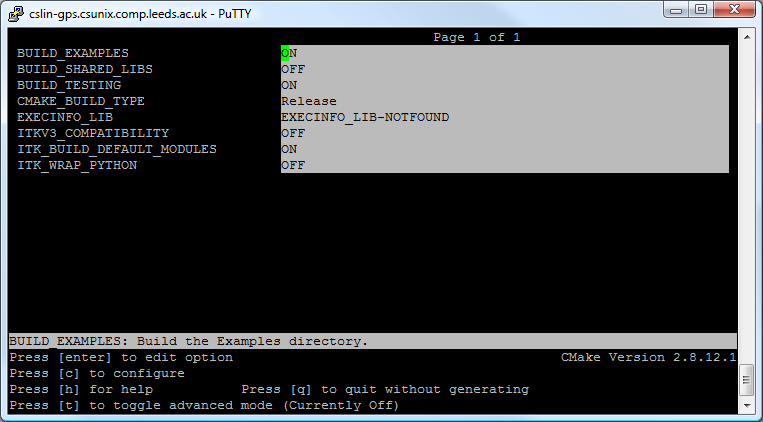
\includegraphics[width=0.8\textwidth]{ccmake-2-8-screenshot.eps}
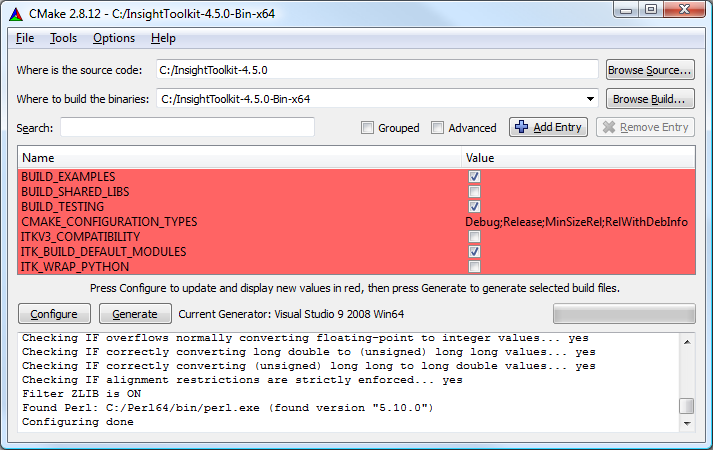
\includegraphics[width=0.8\textwidth]{cmake-gui-2-8-win-screenshot.eps}
\itkcaption[CMake user interface]{CMake user interfaces: at the top is the
interface based on the \code{curses} library supported by UNIX/Linux systems,
below is the Microsoft Windows version of the CMake GUI based on the Qt library
(CMake GUI is also available on UNIX/Linux systems).}
\label{fig:CMakeGUI}
\end{figure}

Running CMake to configure and prepare for compilation a new project initially
requires two pieces of information: where the source code directory is located,
and where the compiled code is to be produced. These are referred to as the
\emph{source directory} and the \emph{binary directory} respectively.
We recommend setting the binary directory to be different than the source
directory in order to produce an \emph{out-of-source} build.

If you choose to use the terminal-based version of CMake (\code{ccmake}) the
binary directory needs to be created first and then CMake is invoked from the
binary directory with the path to the source directory. For example:

\small
\begin{minted}[baselinestretch=1,fontsize=\footnotesize,linenos=false,bgcolor=ltgray]{bash}
mkdir ITK-build
cd ITK-build
ccmake ../ITK
\end{minted}
\normalsize

In the GUI version of CMake (\code{cmake-gui}) the source and binary directories
are specified in the appropriate input fields (Figure \ref{fig:CMakeGUI}) and
the application will request a confirmation to create a new binary directory if
it does not exist.

CMake runs in an interactive mode which allows iterative selection of options
followed by configuration according to the updated options. This iterative
process proceeds until no more options remain to be specified. At this point, a
generation step produces the appropriate build files for your configuration.

This interactive configuration process can be better understood by imagining
the traversal of a path in a decision tree. Every selected option introduces the
possibility that new, dependent options may become relevant. These new options
are presented by CMake at the top of the options list in its interface. Only
when no new options appear after a configuration iteration can you be sure that
the necessary decisions have all been made. At this point build files are
generated for the current configuration.

\subsection{Configuring ITK}
\label{sec:ConfigureITK}

\index{ITK!configuration}

Start terminal-based CMake interface \code{ccmake} on Linux and UNIX, or the
graphical user interface \code{cmake-gui} on Microsoft Windows. Remember to run
\code{ccmake} from the binary directory on Linux and UNIX. On Windows, specify
the source and binary directories in the GUI, then set and modify the
configuration and build option in the interface as necessary.

The examples distributed with the toolkit provide a helpful resource for
learning how to use ITK components but are not essential for compiling the
toolkit itself. The testing section of the source tree includes a large number
of small programs that exercise the capabilities of ITK classes. Enabling the
compilation of the examples and unit tests will considerably increase the build
time. In order to speed up the build process, you can disable the compilation of
the unit tests and examples. This is done by setting the variables
\code{BUILD\_TESTING} and \code{BUILD\_EXAMPLES} to \code{OFF}.

Most CMake variables in ITK have sensible default values. Each time a CMake
variable is changed, it is necessary to re-run the configuration step. In the
terminal-based version of the interface the configuration step is triggered by
hitting the ``c'' key. In the GUI version this is done by clicking on the
``Configure'' button.

When no new options appear highlighted in CMake, you can proceed to generate
Makefiles, a Visual Studio workspace or other appropriate build files depending
on your preferred development environment. This is done in the GUI interface by
clicking on the ``Generate'' button. In the terminal-based version this is done
by hitting the ``g'' key. After the generation process the terminal-based
version of CMake will quit silently. The GUI window of CMake can be left open
for further refinement of configuration options as described in the next
section. With this scenario it is important to generate new build files to
reflect the latest configuration changes. In addition, the new build files need
to be reloaded if the project is open in the integrated development environment
such as Visual Studio or Eclipse.

\subsection{Advanced Module Configuration}
\label{sec:ModuleConfiguration}

\index{ITK!advanced configuration}
\index{ITK!modules}

Following the default configuration introduced in \ref{sec:ConfigureITK},
the majority of the toolkit will be built. The modern modular structure of the
toolkit makes it possible to customize the ITK library by choosing which modules
to include in the build. ITK was officially modularized in version 4.0.0
released in December of 2011. Developers have been testing and improving the
modular structure since then. The toolkit currently contains more than 100
regular/internal modules and many remote modules, while new ITK modules are
being developed.

\code{ITK\_BUILD\_DEFAULT\_MODULES} is the CMake option to build all default
modules in the toolkit, by default this option is \code{ON} as shown in Figure
\ref{fig:CMakeGUI}. The default modules include most internal ITK modules except
the ones that depend on external third party libraries (such as
\code{ITKVtkGlue}, \code{ITKBridgeOpenCV}, \code{ITKBridgeVXL}, etc.) and
several modules containing legacy code (\code{ITKReview}, \code{ITKDeprecated}
and \code{ITKv3Compatibility}).

Apart from the default mode of selecting the modules for building the ITK
library there are two other approaches module selection: the group mode, and the
advanced module mode. When \code{ITK\_BUILD\_DEFAULT\_MODULES} is set to
\code{OFF}, the selection of modules to be included in the ITK library can be
customized by changing the variables enabling group and advanced module
selection.

\code{ITKGroup\_\{group name\}} variables for group module selection are visible
when \code{ITK\_BUILD\_DEFAULT\_MODULES} is \code{OFF}. The ITK source code tree
is organized in such way that a group of modules characterised by close
relationships or similar functionalities stay in one subdirectory. Currently
there are 11 groups (excluding the External and Remote groups). The CMake
\code{ITKGroup\_\{group name\}} options are created for the convenient enabling
or disabling of multiple modules at once. The \code{ITKGroup\_Core} group is
selected by default as shown in Figure \ref{fig:ConfigITKGroup}. When a group is
selected, all modules in the group and their depending modules are enabled. When
a group variable is set to \code{OFF}, all modules in the group, except the ones
that are required by other enabled modules, are disabled.

\begin{figure}[htb!]
\centering
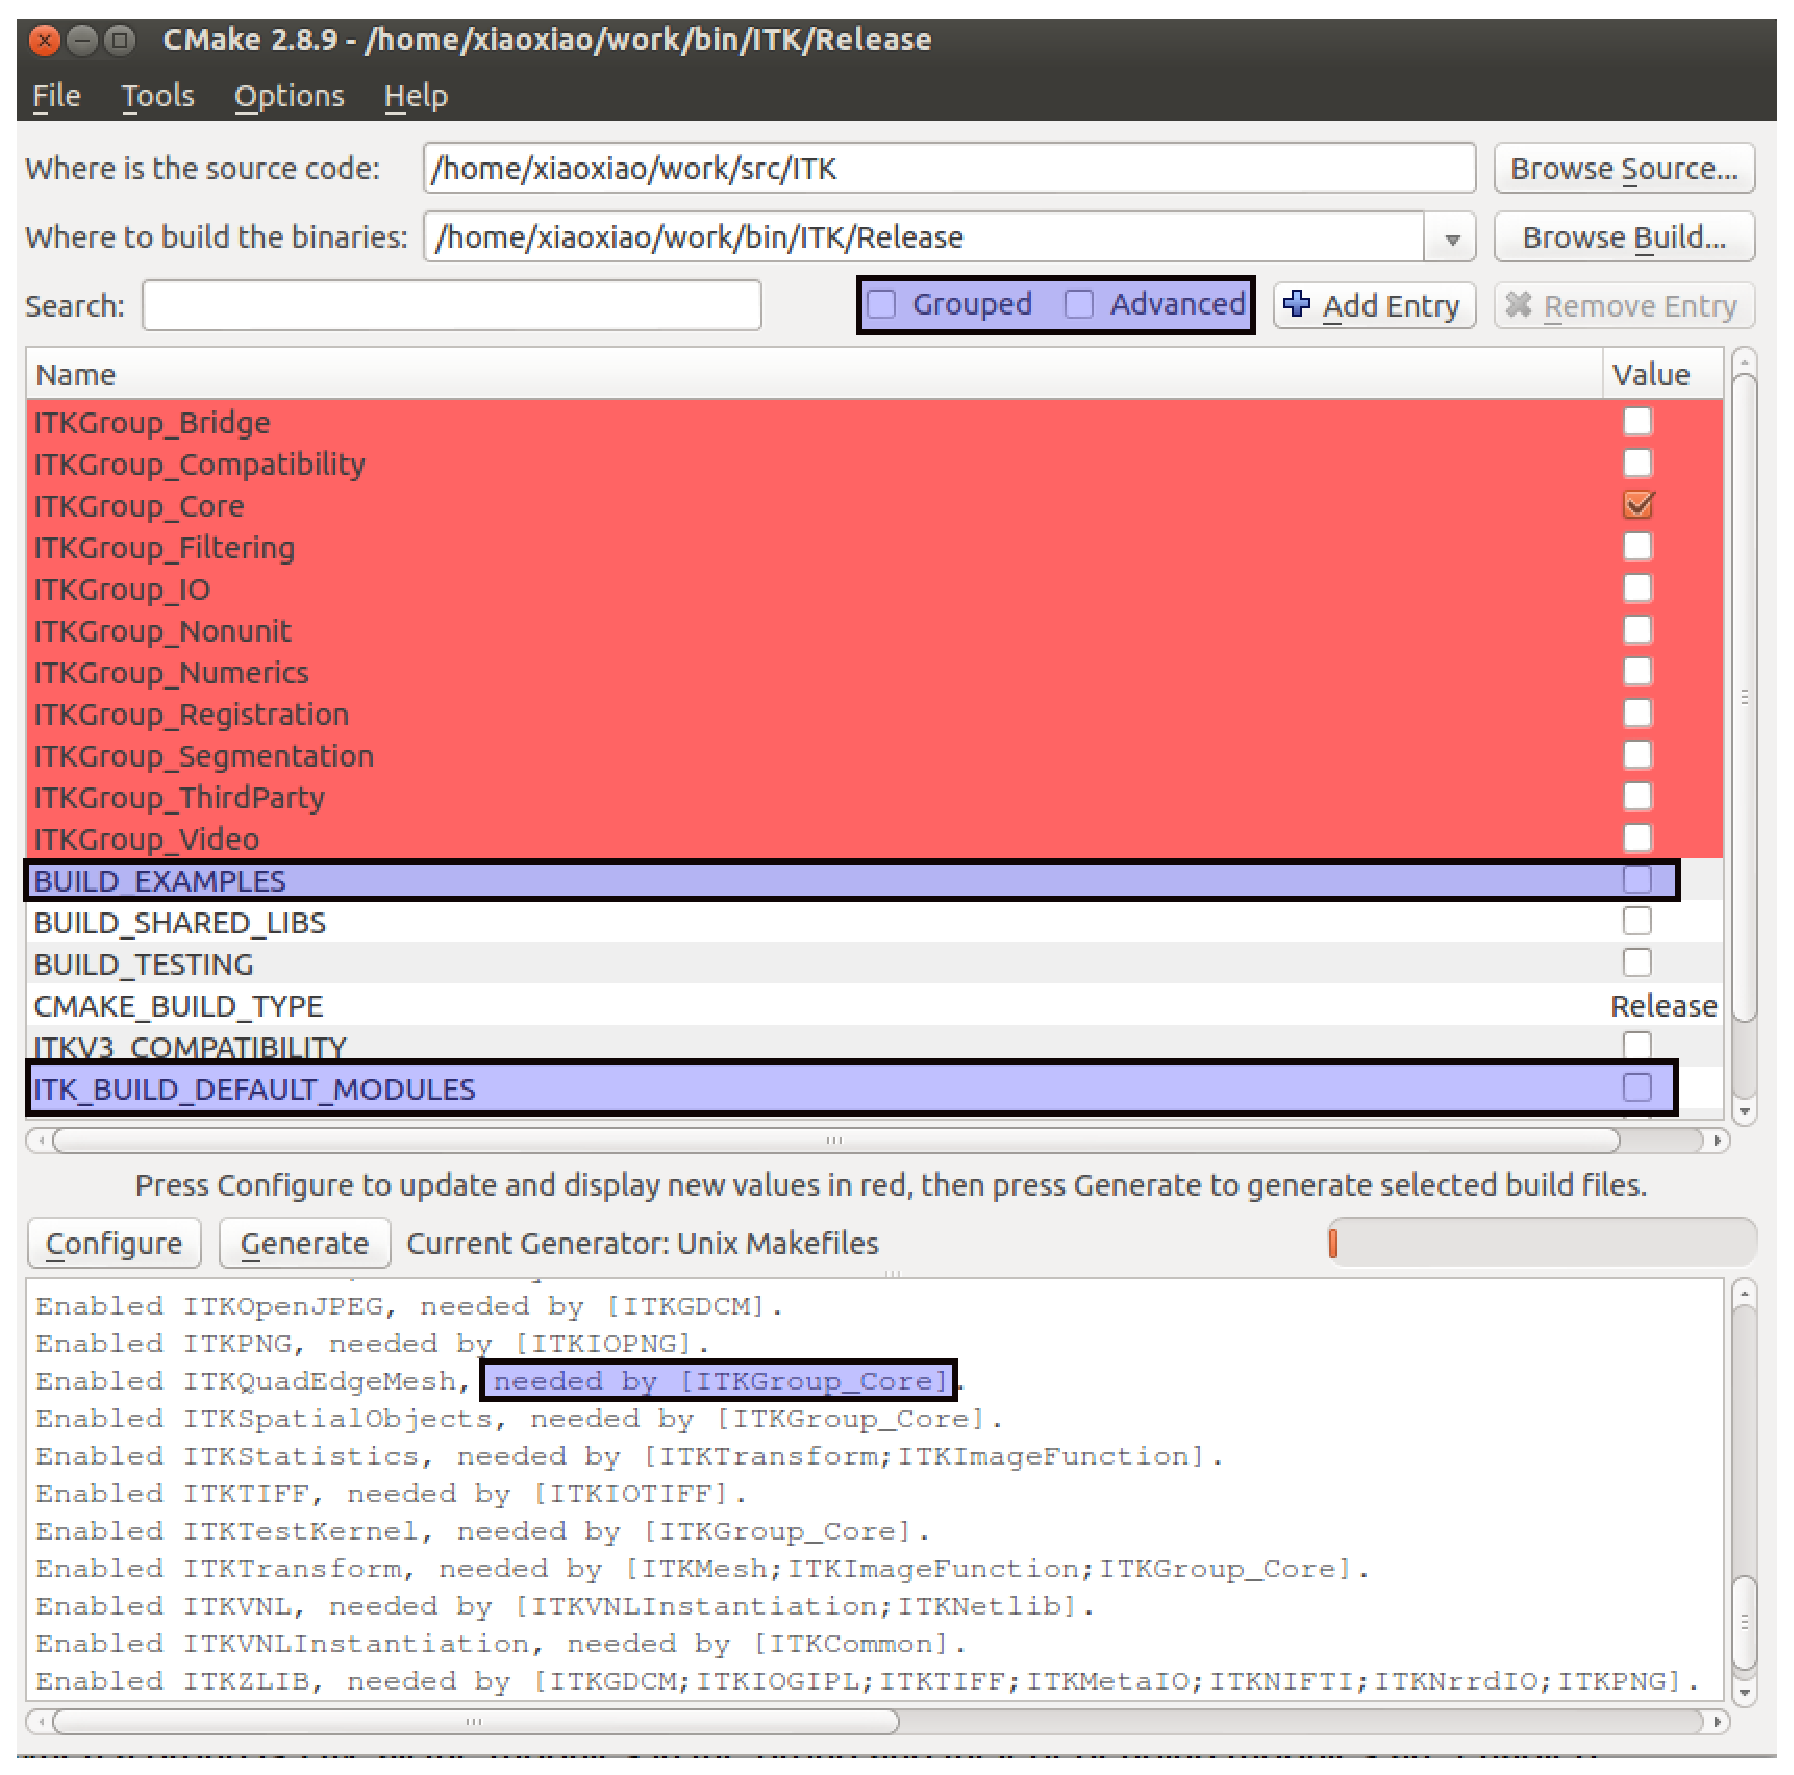
\includegraphics[width=0.8\textwidth]{Configure_ITK_Group.eps}
\itkcaption[ITK Group Configuration]{CMake GUI shows the ITK Group options.}
\label{fig:ConfigITKGroup}
\end{figure}

If you are not sure about which groups to turn on, but you do have a list of
specific modules to be included in your ITK library, you can certainly skip the
Group options and use the \code{Module\_\{module name\}} options only. Whatever
modules you select, their dependent modules are automatically enabled. In the
advanced mode of the CMake GUI, you can manually toggle the build of the
non-default modules via the \code{Module\_\{module name\}} variables. In Figure
\ref{fig:ConfigITKDefault} all default modules' \code{Module\_\{module name\}}
variables are shown disabled for toggling since they are enabled via the
\code{ITK\_BUILD\_DEFAULT\_MODULES} set to \code{ON} variable.

\begin{figure}[htb!]
\centering
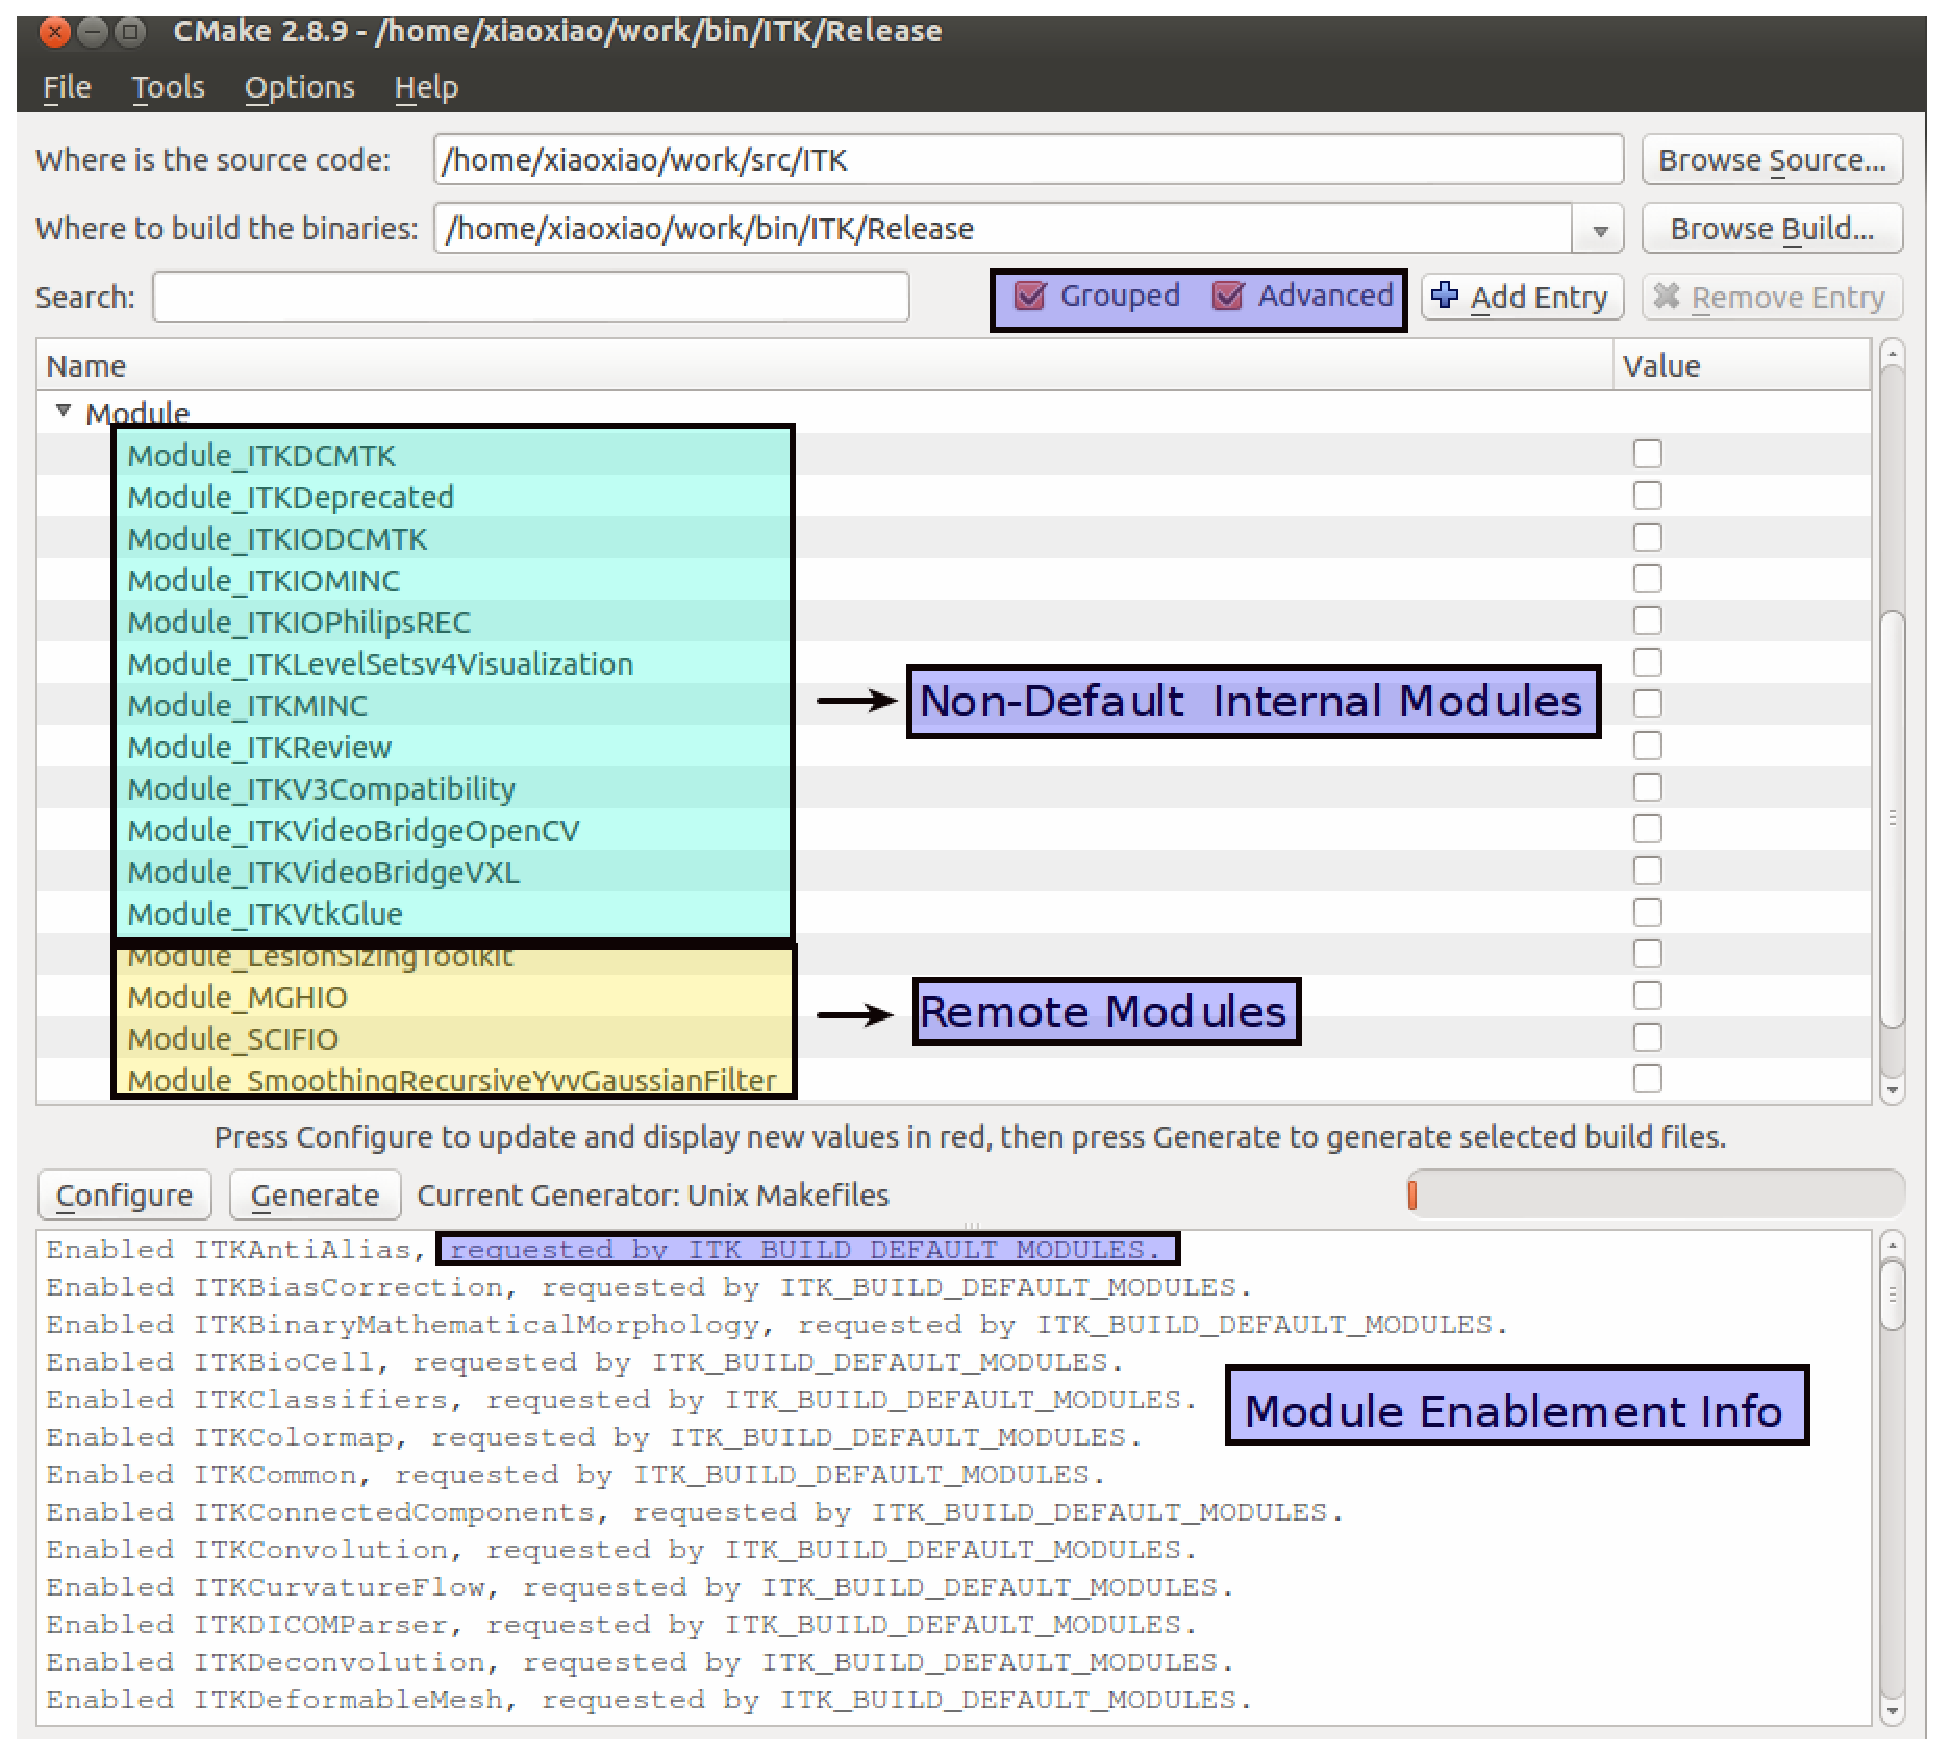
\includegraphics[width=0.8\textwidth]{Configure_ITK_Default.eps}
\itkcaption[Default ITK Configuration]{CMake GUI for configuring ITK: the
advanced mode shows options for non-default ITK Modules.}
\label{fig:ConfigITKDefault}
\end{figure}

However, not all modules will be visible in the CMake GUI at all times due to
the various levels of controls in the previous two modes. If some modules are
already enabled by other modes, these modules are set as internal variables and
are hidden in the CMake GUI. For example, \code{Module\_ITKFoo} variable is
hidden when the module \code{ITKFoo} is enabled in either of the following
scenarios:
\begin{enumerate}
\item module \code{ITKBar} is enabled and depends on \code{ITKFoo},
\item \code{ITKFoo} belongs to the group \code{ITKGroup\_FooAndBar} and the
group is enabled
\item \code{ITK\_BUILD\_DEFAULT\_MODULES} is \code{ON} and \code{ITKFoo} is a
default module.
\end{enumerate}

To find out why a particular module is enabled, check the CMake configuration
messages where the information about enabling or disabling the modules is
displayed (Figure \ref{fig:ConfigITKDefault}); these messages are sorted in
alphabetical order by module names.

\subsection{Compiling ITK}
\label{sec:BuildITK}

\index{ITK!building}

To initiate the build process after generating the build files on Linux or UNIX,
simply type \code{make} in the terminal if the current directory is set to the
ITK binary directory. If using Visual Studio, first load the workspace named
\code{ITK.sln} from the binary directory specified in the CMake GUI and then
start the build by selecting ``Build Solution'' from the ``Build'' menu
or right-clicking on the \code{ALL\_BUILD} target in the Solution Explorer pane
and selecting the ``Build'' context menu item.

The build process can take anywhere from 15 minutes to a couple of hours,
depending on the the build configuration and the performance of your
system. If testing is enabled as part of the normal build process,
about 2400 test programs will be compiled. In this case, you will then need
to run \code{ctest} to verify that all the components of ITK have been correctly built
on your system.

\subsection{Installing ITK on Your System}
\label{sec:Installation}

\index{ITK!installation}

When the build process is complete an ITK binary distribution package can be
generated for installation on your system or on a system with compatible
specifications (such as hardware platform and operating system) as well as
suitable development environment components (such as C++ compiler and CMake).
The default prefix for installation destination directory needs to be specified
during CMake configuration process prior to compiling ITK. The installation
destination prefix can to be set through the CMake cache variable
\code{CMAKE\_INSTALL\_PREFIX}.

Typically distribution packages are generated to provide a ``clean'' form of the
software which is isolated from the details of the build process (separate from
the source and build trees). Due to the intended use of ITK as a toolkit for
software development the step of generating ITK binary packages for installing
ITK on other systems has limited application and thus it can be treated as
optional. However, the step for generating binary distribution packages has a
much wide application for distributing software developed with ITK. Further
details on configuring and generating binary packages with CMake can be found in
the CMake tutorial\footnote{
\url{http://www.cmake.org/cmake/help/cmake_tutorial.html}}.

\section{Getting Started With ITK}
\label{sec:GettingStartedWithITK}

The simplest way to create a new project with ITK is to create two new
directories somewhere in your disk, one to hold the source code and one to
hold the binaries and other files that are created in the build process. For
this example, create a \code{HelloWorldITK} directory to hold the source and a
\code{HelloWorldITK-build} directory to hold the binaries. The first file to
place in the source directory is a \code{CMakeLists.txt} file that will be
used by CMake to generate a Makefile (if you are using Linux or UNIX) or a
Visual Studio workspace (if you are using Microsoft Windows). The second source
file to be created is an actual C++ program that will exercise some of the large
number of classes available in ITK. The details of these files are described in
the following section.

Once both files are in your directory you can run CMake in order to configure
your project. Under UNIX/Linux, you can \code{cd} to your newly created binary
directory and launch the terminal-based version of CMake by entering
``\code{ccmake ../HelloWorldITK}'' in the terminal. Note the
``../HelloWorldITK'' in the command line to indicate that the
\code{CMakeLists.txt} file is up one directory and in \code{HelloWorldITK}.
In CMake GUI which can be used under Microsoft Windows and UNIX/Linux, the
source and binary directories will have to be specified prior to the
configuration and build file generation process.

Both the terminal-based and GUI versions of CMake will require you to specify
the directory where ITK was built in the CMake variable \code{ITK\_DIR}. The ITK
binary directory will contain a file named \code{ITKConfig.cmake} generated
during ITK configuration process with CMake. From this file, CMake will recover
all information required to configure your new ITK project.

After generating the build files, on UNIX/Linux systems the project can be
compiled by typing \code{make} in the terminal provided the current directory
is set to the project's binary directory. In Visual Studio on Microsoft Windows
the project can be built by loading the workspace named \code{HelloWorldITK.sln}
from the binary directory specified in the CMake GUI and selecting
``Build Solution'' from the ``Build'' menu or by right-clicking on
the \code{ALL\_BUILD} target in the Solution Explorer pane and selecting
the ``Build'' context menu item.

The resulting executable, which will be called \code{HelloWorld}, can be
executed on the command line. If on Microsoft Windows, please note that
double-clicking on the icon of the executable will quickly launch a command line
window, run the executable and close the window right away, not giving you time
to see the output. It is therefore preferable to run the executable from the DOS
command line by starting the \code{cmd.exe} shell first.

\subsection{Hello World!}
\label{sec:HelloWorldITK}

\index{Hello World}

This section provides and explains the contents of the two files which need to
be created for your new project. These two files can be found in the
\code{ITK/Examples/Installation} directory.

The \code{CMakeLists.txt} file contains the following lines:

% CMake looks similar to bash with regards to formatting.
\begin{minted}[linenos=false]{bash}
project(HelloWorld)

find_package(ITK REQUIRED)
include(${ITK_USE_FILE})

add_executable(HelloWorld HelloWorld.cxx)

target_link_libraries(HelloWorld ${ITK_LIBRARIES})
\end{minted}

The first line defines the name of your project as it appears in Visual Studio
or Eclipse; this line will have no effect with UNIX/Linux Makefiles. The second
line loads a CMake file with a predefined strategy for finding ITK. If the
strategy for finding ITK fails, CMake will report an error which can be
corrected by providing the location of the directory where ITK was compiled or
installed on your system. In this case the path to the ITK's binary/installation
directory needs to be specified as the value of the \code{ITK\_DIR} CMake
variable. The line \code{include(\$\{USE\_ITK\_FILE\})} loads the
\code{UseITK.cmake} file which contains the configuration information about the
specified ITK build. The line starting with \code{add\_executable} call defines
as its first argument the name of the executable that will be produced
as result of this project. The remaining argument(s) of \code{add\_executable}
are the names of the source files to be compiled. Finally, the
\code{target\_link\_libraries} call specifies which ITK libraries will be
linked against this project. Further details on creating and configuring CMake
projects can be found in the CMake tutorial\footnote{
\url{http://www.cmake.org/cmake/help/cmake\_tutorial.html}} and CMake online
documentation\footnote{\url{http://www.cmake.org/cmake/help/documentation.html}}.

\input HelloWorld.tex

By this point you have successfully configured and compiled ITK, and created
your first simple program! If you have experienced any difficulties while
following the instructions provided in this section, please join the community
mailing list (see Section~\ref{sec:JoinMailList} on
page \pageref{sec:JoinMailList}) and post questions there.

\fi


\part{Architecture}

\ifitkFullVersion
  \chapter{System Overview}
\label{chapter:SystemOverview}

The purpose of this chapter is to provide you with an overview of the
\emph{Insight Toolkit} system. We recommend that you read this chapter to
gain an appreciation for the breadth and area of application of ITK.

\section{System Organization}
\label{sec:SystemOrganization}

The Insight Toolkit consists of several subsystems. A brief
description of these subsystems follows. Later sections in this chapter---and
in some cases additional chapters---cover these concepts in more detail.

\begin{description}
	\item[Essential System Concepts.] Like any software system, ITK is
        built around some core design concepts. Some of the more important
        concepts include generic programming, smart pointers for memory
        management, object factories for adaptable object instantiation,
        event management using the command/observer design paradigm, and
        multithreading support.

	\item[Numerics.] ITK uses VXL's VNL numerics libraries. These are
        easy-to-use C++ wrappers around the Netlib Fortran numerical
        analysis routines \footnote{\url{http://www.netlib.org}}.

	\item[Data Representation and Access.]  Two principal classes are
        used to represent data: the \doxygen{Image} and \doxygen{Mesh}
        classes.  In addition, various types of iterators and containers are
        used to hold and traverse the data. Other important but less popular
        classes are also used to represent data such as \doxygen{Histogram} and
        \doxygen{SpatialObject}.

	\item[Data Processing Pipeline.]  The data representation
	classes (known as \emph{data objects}) are operated on by
	\emph{filters} that in turn may be organized into data flow
	\emph{pipelines}. These pipelines maintain state and therefore
	execute only when necessary.  They also support
	multi-threading, and are streaming capable (i.e., can operate
	on pieces of data to minimize the memory footprint).

        \item[IO Framework.] Associated with the data processing
        pipeline are \emph{sources}, filters that initiate the
        pipeline, and \emph{mappers}, filters that terminate the
        pipeline.  The standard examples of sources and mappers are
        \emph{readers} and \emph{writers} respectively.  Readers
        input data (typically from a file), and writers output data
        from the pipeline.

	\item[Spatial Objects.] Geometric shapes are represented in ITK using
        the spatial object hierarchy.  These classes are intended to support
        modeling of anatomical structures. Using a common basic interface,
        the spatial objects are capable of representing regions of space in a
        variety of different ways. For example: mesh structures, image masks,
        and implicit equations may be used as the underlying representation
        scheme.  Spatial objects are a natural data structure for
        communicating the results of segmentation methods and for introducing
        anatomical priors in both segmentation and registration methods.

	\item[Registration Framework.] A flexible framework for registration
        supports four different types of registration: image registration,
        multiresolution registration, PDE-based registration, and FEM (finite
        element method) registration.

	\item[FEM Framework.] ITK includes a subsystem for solving general
        FEM problems, in particular non-rigid registration. The FEM package
        includes mesh definition (nodes and elements), loads, and boundary
        conditions.

	\item[Level Set Framework.] The level set framework is a set of
        classes for creating filters to solve partial differential equations
        on images using an iterative, finite difference update scheme. The
        level set framework consists of finite difference solvers including a
        sparse level set solver, a generic level set segmentation filter, and
        several specific subclasses including threshold, Canny, and Laplacian
        based methods.

	\item[Wrapping.] ITK uses a unique, powerful system for
	producing interfaces (i.e., ``wrappers'') to interpreted
	languages such as Python. The GCC-XML\footnote{\url{http://gccxml.org}}
        tool is used to produce an XML description of arbitrarily complex C++ code.
	An interface generator script is then used to transform the XML description
        into wrappers using the SWIG\footnote{\url{http://www.swig.org/}} package.

        \item[Utilities] Several auxiliary subsystems are available to
        supplement other classes in the system. For example, calculators are
        classes that perform specialized operations in support of filters
        (e.g., MeanCalculator computes the mean of a sample). Other utilities
        include a partial DICOM parser, MetaIO file support, png, zlib, and
        interfaces to the Visualization Toolkit (VTK) system.
\end{description}


\section{Essential System Concepts}
\label{sec:EssentialSystemConcepts}

This section describes some of the core concepts and implementation features
found in ITK.

\subsection{Generic Programming}
\label{sec:GenericProgramming}

\index{generic programming}
\index{template}

Generic programming is a method of organizing libraries consisting of
generic---or reusable---software components \cite{Musser1996}. The idea is to
make software that is capable of ``plugging together'' in an efficient,
adaptable manner. The essential ideas of generic programming are
\emph{containers} to hold data, \emph{iterators} to access the data, and
\emph{generic algorithms} that use containers and iterators to create
efficient, fundamental algorithms such as sorting. Generic programming is
implemented in C++ with the \emph{template} programming mechanism and the
use of the STL Standard Template Library \cite{Austern1999}.

C++ templating is a programming technique allowing users to write software in
terms of one or more unknown types \code{T}. To create executable code, the
user of the software must specify all types \code{T} (known as \emph{template
instantiation}) and successfully process the code with the compiler. The
\code{T} may be a native type such as
\code{float} or \code{int}, or \code{T} may be a user-defined type (e.g.,
a \code{class}). At compile-time, the compiler makes sure that the templated
types are compatible with the instantiated code and that the types are
supported by the necessary methods and operators.

ITK uses the techniques of generic programming in its implementation. The
advantage of this approach is that an almost unlimited variety of data types
are supported simply by defining the appropriate template types. For example,
in ITK it is possible to create images consisting of almost any type of
pixel. In addition, the type resolution is performed at compile-time, so the
compiler can optimize the code to deliver maximal performance. The
disadvantage of generic programming is that the analysis performed at compile
time increases the time to build an application. Also, the increased
complexity may produce difficult to decipher error messages due to even the
simplest syntax errors. For those unfamiliar with templated code and
generic programming, we recommend the two books cited above.

\subsection{Include Files and Class Definitions}
\label{sec:IncludeFiles}

In ITK classes are defined by a maximum of two files: a header \code{.h} file
and an implementation file---\code{.cxx} if a non-templated class, and a
\code{.hxx} if a templated class.
The header files contain class declarations
and formatted comments that are used by the Doxygen documentation
system to automatically produce HTML manual pages.

In addition to class headers, there are a few other important header files.
\begin{description}
        \item[\code{itkMacro.h}] is found in the
        \code{Modules/Core/Common/include} directory
        and defines standard system-wide macros (such as \code{Set/Get},
        constants, and other parameters).

        \item[\code{itkNumericTraits.h}] is found in the
        \code{Modules/Core/Common/include} directory and defines numeric
        characteristics for native types such as its maximum and minimum
        possible values.
\end{description}

\subsection{Object Factories}
\label{sec:ObjectFactories}

\index{object factory}
\index{factory}

Most classes in ITK are instantiated through an \emph{object factory}
mechanism. That is, rather than using the standard C++ class constructor and
destructor, instances of an ITK class are created with the static class
\code{New()} method. In fact, the constructor and destructor are
\code{protected:} so it is generally not possible to construct an ITK
instance on the stack. (Note: this behavior pertains to classes that are
derived from \doxygen{LightObject}. In some cases the need for speed or
reduced memory footprint dictates that a class not be derived from
LightObject, and in this case instances may be created on the stack. An
example of such a class is \doxygen{EventObject}.)

The object factory enables users to control run-time instantiation of classes
by registering one or more factories with \doxygen{ObjectFactoryBase}. These
registered factories support the method \code{CreateInstance(classname)}
which takes as input the name of a class to create. The factory can choose to
create the class based on a number of factors including the computer system
configuration and environment variables. For example, a particular
application may wish to deploy its own class implemented using
specialized image processing hardware (i.e., to realize a performance
gain). By using the object factory mechanism, it is possible at run-time to
replace the creation of a particular ITK filter with such a custom class. (Of
course, the class must provide the exact same API as the one it is
replacing.) To do this, the user compiles her class (using the same compiler,
build options, etc.) and inserts the object code into a shared library or
DLL. The library is then placed in a directory referred to by the
\code{ITK\_AUTOLOAD\_PATH} environment variable. On instantiation, the object
factory will locate the library, determine that it can create a class of a
particular name with the factory, and use the factory to create the
instance. (Note: if the \code{CreateInstance()} method cannot find a factory
that can create the named class, then the instantiation of the class falls
back to the usual constructor.)

In practice, object factories are used mainly (and generally transparently) by
the ITK input/output (IO) classes. For most users the greatest impact is on
the use of the \code{New()} method to create a class. Generally the
\code{New()} method is declared and implemented via the macro
\code{itkNewMacro()} found in \code{Modules/Core/Common/include/itkMacro.h}.


\subsection{Smart Pointers and Memory Management}
\label{sec:SmartPointers}

\index{smart pointer}

By their nature, object-oriented systems represent and operate on data through
a variety of object types, or classes. When a particular class is
instantiated to produce an instance of that class, memory allocation occurs
so that the instance can store data attribute values and method pointers
(i.e., the vtable). This object may then be referenced by other classes or
data structures during normal operation of the program. Typically, during
program execution, all references to the instance may disappear at which point
the instance must be deleted to recover memory resources. Knowing when to
delete an instance, however, is difficult. Deleting the instance too soon
results in program crashes; deleting it too late causes memory leaks (or
excessive memory consumption). This process of allocating and
releasing memory is known as memory management.

In ITK, memory management is implemented through reference counting. This
compares to another popular approach---garbage collection---used
\index{garbage collection} by many
systems, including Java. In reference counting, a count of the number of
references to each instance is kept. When the reference goes to zero, the
object destroys itself. In garbage collection, a background process sweeps
the system identifying instances no longer referenced in the system and
deletes them. The problem with garbage collection is that the actual point in
time at which memory is deleted is variable. This is unacceptable when an
object size may be gigantic (think of a large 3D volume gigabytes in
size). Reference counting deletes memory immediately (once all references to
an object disappear).

Reference counting is implemented through a \code{Register()}/\code{Delete()}
member function interface.  All instances of an ITK object have a
\code{Register()} method invoked on them by any other object that references
an them. The \code{Register()} method increments the instances' reference
count. When the reference to the instance disappears, a \code{Delete()}
method is invoked on the instance that decrements the reference count---this
is equivalent to an \code{UnRegister()} method. When the reference count
returns to zero, the instance is destroyed.

This protocol is greatly simplified by using a helper class called a
\doxygen{SmartPointer}. The smart pointer acts like a regular pointer
(e.g. supports operators \code{->} and \code{*}) but automagically performs a
\code{Register()} when referring to an instance, and an \code{UnRegister()}
when it no longer points to the instance.  Unlike most other instances in
ITK, SmartPointers can be allocated on the program stack, and are
automatically deleted when the scope that the SmartPointer was created
is closed. As a result, you should \emph{rarely if ever call Register() or
Delete()} in ITK. For example:

\small
\begin{verbatim}
  MyRegistrationFunction()
    { <----- Start of scope

    // here an interpolator is created and associated to the
    // SmartPointer "interp".
    InterpolatorType::Pointer interp = InterpolatorType::New();

    } <------ End of scope
\end{verbatim}
\normalsize

In this example, reference counted objects are created (with the \code{New()}
method) with a reference count of one. Assignment to the SmartPointer
\code{interp} does not change the reference count. At the end of scope,
\code{interp} is destroyed, the reference count of the actual interpolator
object (referred to by \code{interp}) is decremented, and if it reaches zero,
then the interpolator is also destroyed.

Note that in ITK SmartPointers are always used to refer to instances of
classes derived from \doxygen{LightObject}. Method invocations and function
calls often return ``real'' pointers to instances, but they are immediately
assigned to a SmartPointer. Raw pointers are used for non-LightObject classes when
the need for speed and/or memory demands a smaller, faster class. Raw pointers
are preferred for multi-threaded sections of code.


\subsection{Error Handling and Exceptions}
\label{sec:ErrorHandling}

\index{exceptions}
\index{error handling}

In general, ITK uses exception handling to manage errors during program
execution. Exception handling is a standard part of the C++ language and
generally takes the form as illustrated below:
\small
\begin{verbatim}
  try
    {
    //...try executing some code here...
    }
  catch ( itk::ExceptionObject & exp )
    {
    //...if an exception is thrown catch it here
    }
\end{verbatim}
\normalsize

where a particular class may throw an exception as demonstrated below (this
code snippet is taken from \doxygen{ByteSwapper}:
\small
\begin{verbatim}
  switch ( sizeof(T) )
    {
    //non-error cases go here followed by error case
    default:
      ByteSwapperError e(__FILE__, __LINE__);
      e.SetLocation("SwapBE");
      e.SetDescription("Cannot swap number of bytes requested");
      throw e;
    }
\end{verbatim}
\normalsize

Note that \doxygen{ByteSwapperError} is a subclass of
\doxygen{ExceptionObject}. In fact, all ITK exceptions derive
from ExceptionObject. In this example a special constructor and C++
preprocessor variables \code{\_\_FILE\_\_} and \code{\_\_LINE\_\_} are used to instantiate
the exception object and provide additional information to the user. You can
choose to catch a particular exception and hence a specific ITK error, or you
can trap \emph{any} ITK exception by catching ExceptionObject.


\subsection{Event Handling}
\label{sec:EventHandling}

\index{event handling}
\index{Command/Observer design pattern}
\index{itk::Command}
\index{ProgressEvent()}
\index{InvokeEvent()}

Event handling in ITK is implemented using the Subject/Observer design
pattern \cite{Gamma1995} (sometimes referred to as the Command/Observer
design pattern). In this approach, objects indicate that they are watching
for a particular event---invoked by a particular instance---by registering
with the instance that they are watching.  For example, filters in ITK
periodically invoke the \doxygen{ProgressEvent}. Objects that have registered
their interest in this event are notified when the event occurs. The
notification occurs via an invocation of a command (i.e., function callback,
method invocation, etc.) that is specified during the registration
process. (Note that events in ITK are subclasses of EventObject; look
in \code{itkEventObject.h} to determine which events are available.)

To recap via example: various objects in ITK will invoke specific events
as they execute (from ProcessObject):
\small
\begin{verbatim}
  this->InvokeEvent( ProgressEvent() );
\end{verbatim}
\normalsize

To watch for such an event, registration is required that associates a
command (e.g., callback function) with the event:
\code{Object::AddObserver()} method:
\small
\begin{verbatim}
  unsigned long progressTag =
    filter->AddObserver(ProgressEvent(), itk::Command*);
\end{verbatim}
\normalsize

When the event occurs, all registered observers are notified via invocation
of the associated \code{Command::Execute()} method. Note that several
subclasses of Command are available supporting const and
non-const member functions as well as C-style functions. (Look in
\code{Modules/Core/Common/include/itkCommand.h} to find pre-defined subclasses of
Command. If nothing suitable is found, derivation is another
possibility.)

\subsection{Multi-Threading}
\label{sec:MultiThreading}

Multithreading is handled in ITK through a high-level design
abstraction. This approach provides portable multithreading and hides the
complexity of differing thread implementations on the many systems supported
by ITK. For example, the class \doxygen{MultiThreader} provides support for
multithreaded execution using \code{sproc()} on an SGI, or
\code{pthread\_create} on any platform supporting POSIX threads.

Multithreading is typically employed by an algorithm during its execution
phase. MultiThreader can be used to execute a single method on
multiple threads, or to specify a method per thread. For example, in the
class \doxygen{ImageSource} (a superclass for most image processing filters)
the \code{GenerateData()} method uses the following methods:

\small
\begin{verbatim}
  multiThreader->SetNumberOfThreads(int);
  multiThreader->SetSingleMethod(ThreadFunctionType, void* data);
  multiThreader->SingleMethodExecute();
\end{verbatim}
\normalsize

In this example each thread invokes the same method. The multithreaded filter
takes care to divide the image into different regions that do not overlap for
write operations.

The general philosophy in ITK regarding thread safety is that accessing
different instances of a class (and its methods) is a thread-safe operation.
Invoking methods on the same instance in different threads is to be avoided.


\section{Numerics}
\label{sec:Numerics}

\index{VNL}
\index{numerics}

ITK uses the VNL numerics library to provide resources for numerical
programming combining the ease of use of packages like Mathematica and Matlab
with the speed of C and the elegance of C++. It provides a C++ interface to
the high-quality Fortran routines made available in the public domain by
numerical analysis researchers. ITK extends the functionality of VNL
by including interface classes between VNL and ITK proper.

The VNL numerics library includes classes for
\begin{description}
        \item[Matrices and vectors.] Standard matrix and vector support
        and operations on these types.

        \item[Specialized matrix and vector classes.] Several special matrix
        and vector class with special numerical properties are
        available. Class \code{vnl\_diagonal\_matrix} provides a fast and
        convenient diagonal matrix, while fixed size matrices and vectors
        allow "fast-as-C" computations (see \code{vnl\_matrix\_fixed<T,n,m>}
        and example subclasses \code{vnl\_double\_3x3} and
        \code{vnl\_double\_3}).

        \item[Matrix decompositions.] Classes \code{vnl\_svd<T>},
        \code{vnl\_symmetric\_eigensystem<T>}, and
        \code{vnl\_generalized\_eigensystem}.

        \item[Real polynomials.] Class \code{vnl\_real\_polynomial} stores
        the coefficients of a real polynomial, and provides methods of
        evaluation of the polynomial at any x, while class
        \code{vnl\_rpoly\_roots} provides a root finder.

        \item[Optimization.] Classes \code{vnl\_levenberg\_marquardt},
        \code{vnl\_amoeba}, \code{vnl\_conjugate\_gradient},
        \code{vnl\_lbfgs} allow optimization of user-supplied
        functions either with or without user-supplied derivatives.

        \item[Standardized functions and constants.] Class \code{vnl\_math}
        defines constants (pi, e, eps...) and simple functions (sqr, abs,
        rnd...). Class \code{numeric\_limits} is from the ISO standard
        document, and provides a way to access basic limits of a
        type. For example \code{numeric\_limits<short>::max()} returns the maximum
        value of a short.
\end{description}

Most VNL routines are implemented as wrappers around the high-quality Fortran
routines that have been developed by the numerical analysis community over
the last forty years and placed in the public domain. The central repository
for these programs is the "netlib" server \footnote{\url{http://www.netlib.org/}}. The
National Institute of Standards and Technology (NIST) provides an excellent
search interface to this repository in its \emph{Guide to Available Mathematical
Software (GAMS)}\footnote{\url{http://gams.nist.gov}}, both as a decision tree and a
text search.

ITK also provides additional numerics functionality. A suite of optimizers, that
use VNL under the hood and integrate with the registration framework
are available. A large collection of statistics functions---not available from
VNL---are also provided in the \code{Insight/Numerics/Statistics}
directory. In addition, a complete finite element (FEM) package is available,
primarily to support the deformable registration in ITK.


\section{Data Representation}
\label{sec:DataRepresentationAndAccess}
%	mesh, image, iterators, various containers

\index{data object}

There are two principle types of data represented in ITK: images and
meshes. This functionality is implemented in the classes
Image and Mesh, both of which are subclasses of
\doxygen{DataObject}. In ITK, data objects are classes that are meant to
be passed around the system and may participate in data flow pipelines (see
Section~\ref{sec:DataProcessingPipeline} on
page~\pageref{sec:DataProcessingPipeline} for more information).


\index{itk::Image}

\doxygen{Image} represents an \emph{n}-dimensional, regular sampling of
data. The sampling direction is parallel to direction matrix axes, and
the origin of the sampling, inter-pixel spacing, and the number of samples in
each direction (i.e., image dimension) can be specified. The sample, or
pixel, type in ITK is arbitrary---a template parameter \code{TPixel}
specifies the type upon template instantiation. (The dimensionality of the
image must also be specified when the image class is instantiated.) The key
is that the pixel type must support certain operations (for example, addition
or difference) if the code is to compile in all cases (for example, to be
processed by a particular filter that uses these operations). In practice,
most applications will use a C++ simple type (e.g., \code{int}, \code{float})
or a pre-defined pixel type and will rarely create a new type of pixel class.

One of the important ITK concepts regarding images is that rectangular,
continuous pieces of the image are known as \emph{regions}. Regions are used
to specify which part of an image to process, for example in multithreading,
or which part to hold in memory. In ITK there are three common types of
regions:
\begin{enumerate}
\item \code{LargestPossibleRegion}---the image in its entirety.
\item \code{BufferedRegion}---the portion of the image retained in memory.
\item \code{RequestedRegion}---the portion of the region requested by a
filter or other class when operating on the image.
\end{enumerate}

\index{itk::Mesh}

The Mesh class represents an \emph{n}-dimensional, unstructured grid. The
topology of the mesh is represented by a set of \emph{cells} defined by a type
and connectivity list; the connectivity list in turn refers to points.  The
geometry of the mesh is defined by the \emph{n}-dimensional points in
combination with associated cell interpolation functions. \code{Mesh} is
designed as an adaptive representational structure that changes depending on
the operations performed on it. At a minimum, points and cells are required in
order to represent a mesh; but it is possible to add additional topological
information.  For example, links from the points to the cells that use each
point can be added; this provides implicit neighborhood information assuming
the implied topology is the desired one. It is also possible to specify
boundary cells explicitly, to indicate different connectivity from the implied
neighborhood relationships, or to store information on the boundaries of
cells.

The mesh is defined in terms of three template parameters: 1) a pixel type
associated with the points, cells, and cell boundaries; 2) the dimension of
the points (which in turn limits the maximum dimension of the cells); and 3)
a ``mesh traits'' template parameter that specifies the types of the
containers and identifiers used to access the points, cells, and/or
boundaries. By using the mesh traits carefully, it is possible to create
meshes better suited for editing, or those better suited for ``read-only''
operations, allowing a trade-off between representation flexibility, memory,
and speed.

Mesh is a subclass of \doxygen{PointSet}. The PointSet
class can be used to represent point clouds or randomly distributed
landmarks, etc. The PointSet class has no associated topology.


\section{Data Processing Pipeline}
\label{sec:DataProcessingPipeline}

\index{data processing pipeline}

\index{process object}
\index{source}
\index{reader}
\index{filter}
\index{mapper}

While data objects (e.g., images and meshes) are used to represent data,
\emph{process objects} are classes that operate on data objects and may
produce new data objects. Process objects are classed as
\emph{sources}, \emph{filter objects}, or \emph{mappers}.  Sources (such as
readers) produce data, filter objects take in data and process it to produce
new data, and mappers accept data for output either to a file or
some other system.  Sometimes the term \emph{filter} is used broadly
to refer to all three types.

\index{streaming}

The data processing pipeline ties together data objects (e.g., images and
meshes) and process objects. The pipeline supports an automatic updating
mechanism that causes a filter to execute if and only if its input
or its internal state changes. Further, the data pipeline supports
\emph{streaming}, the ability to automatically break data into smaller
pieces, process the pieces one by one, and reassemble the processed data into
a final result.

Typically data objects and process objects are connected together using the
\code{SetInput()} and \code{GetOutput()} methods as follows:

\small
\begin{verbatim}
  typedef itk::Image<float,2> FloatImage2DType;

  itk::RandomImageSource<FloatImage2DType>::Pointer random;
  random = itk::RandomImageSource<FloatImage2DType>::New();
  random->SetMin(0.0);
  random->SetMax(1.0);

  itk::ShrinkImageFilter<FloatImage2DType,FloatImage2DType>::Pointer shrink;
  shrink = itk::ShrinkImageFilter<FloatImage2DType,FloatImage2DType>::New();
  shrink->SetInput(random->GetOutput());
  shrink->SetShrinkFactors(2);

  itk::ImageFileWriter<FloatImage2DType>::Pointer writer;
  writer = itk::ImageFileWriter<FloatImage2DType>::New();
  writer->SetInput (shrink->GetOutput());
  writer->SetFileName( ``test.raw'' );
  writer->Update();
\end{verbatim}
\normalsize

In this example the source object \doxygen{RandomImageSource} is connected
to the \doxygen{ShrinkImageFilter}, and the shrink filter is connected to
the mapper \doxygen{ImageFileWriter}. When the \code{Update()} method is
invoked on the writer, the data processing pipeline causes each of these
filters in order, culminating in writing the final data to a file on disk.

%\section{Registration Framework}
%\label{sec:RegistrationFramework}
%
%blah blah
%
%\section{FEM Framework}
%\label{sec:FEMFramework}
%
%blah blah
%
\section{Spatial Objects}
\label{sec:SpatialObjectsOverview}
\index{spatial object}
%
The ITK spatial object framework supports the philosophy that the task of
image segmentation and registration is actually the task of object
processing. The image is but one medium for representing objects of interest,
and much processing and data analysis can and should occur at the object
level and not based on the medium used to represent the object.

ITK spatial objects provide a common interface for accessing the physical
location and geometric properties of and the relationship between objects in
a scene that is independent of the form used to represent those objects. That
is, the internal representation maintained by a spatial object may be a list
of points internal to an object, the surface mesh of the object, a continuous
or parametric representation of the object's internal points or surfaces, and
so forth.

The capabilities provided by the spatial objects framework supports their use
in object segmentation, registration, surface/volume rendering, and other
display and analysis functions. The spatial object framework extends the
concept of a ``scene graph'' \index{scene graph} that is common to computer rendering packages so
as to support these new functions. With the spatial objects framework you
can:
\begin{enumerate}

        \item Specify a spatial object's parent and children objects.  In
        this way, a liver may contain vessels and those vessels can be
        organized in a tree structure.

        \item Query if a physical point is inside an object or
        (optionally) any of its children.

        \item Request the value and derivatives, at a physical point,
        of an associated intensity function, as specified
        by an object or (optionally) its children.

        \item Specify the coordinate transformation that maps a parent
        object's coordinate system into a child object's coordinate system.

        \item Compute the bounding box of a spatial object and (optionally)
        its children.

        \item Query the resolution at which the object was originally
        computed.  For example, you can query the resolution (i.e., voxel
        spacing) of the image used to generate a particular instance of a
        \doxygen{BlobSpatialObject}.
\end{enumerate}

Currently implemented types of spatial objects include: Blob, Ellipse, Group,
Image, Line, Surface, and Tube.  The \doxygen{Scene} object is used to hold
a list of spatial objects that may in turn have children.  Each spatial
object can be assigned a color property.  Each spatial object type has its
own capabilities. For example, \doxygen{TubeSpatialObject}s indicate to what
point on their parent tube they connect.

There are a limited number of spatial objects and their methods in ITK, but
their number is growing and their potential is huge. Using the nominal
spatial object capabilities, methods such as marching cubes or mutual
information registration, can be applied to objects regardless of their
internal representation. By having a common API, the same method can be used
to register a parametric representation of a heart with an individual's CT
data or to register two hand segmentations of a liver.

%blah blah
%
%\section{Level Set Framework}
%\label{sec:LevelSetFramework}
%
%blah blah
%
\section{Wrapping}
\label{sec:Wrapping}

\index{wrapping}
\index{Tcl}
\index{Python}

While the core of ITK is implemented in C++, Python bindings can be
automatically generated and ITK programs can be created using these
programming languages. This capability is under active development and is for
the advanced users only. However, this brief description will give an idea
of what is possible and where to look for those who are interested in this facility.

The wrapping process in ITK is quite complex due to the use of generic
programming (i.e., extensive use of C++ templates). Systems like VTK that use
their own wrapping facility are non-templated and customized to the coding
methodology found in the system. Even systems like SWIG that are designed
for general wrapper generation have difficulty with ITK code because general
C++ is difficult to parse. As a result, the ITK wrapper generator uses a
combination of tools to produce language bindings.

\begin{enumerate}
  \item gccxml is a modified version of the GNU compiler gcc that
    produces an XML description of an input C++ program.
  \item The \code{igenerator.py} script in the ITK source tree processes XML
    information produced by gccxml and generates standard input files
    (\code{*.i} files) to the next tool (SWIG), indicating what is to be wrapped
    and how to wrap it.
  \item SWIG produces the appropriate language bindings (such as Python).
\end{enumerate}

To learn more about the wrapping process, please see the \code{Wrapping}
directory. The wrapping process is orchestrated by a number of CMake macros
found in the \code{Wrapping} directory.  The result of the wrapping process is
a set of shared libraries (.so in Linux or .dlls on Windows) that can be used
by interpreted languages.

There is almost a direct translation from C++, with the differences being the
particular syntactical requirements of each language. For example, in the
directory \code{Examples/IO}, the test \code{DicomSliceRead.py} has a code
fragment that appears as follows:
\small
\begin{verbatim}
  InputImageType = itk.Image.SS2
  OutputImageType = itk.Image.UC2

  reader = itk.ImageFileReader[InputImageType].New()
  reader.SetFileName(sys.argv[1])

  filter = itk.RescaleIntensiteImageFilter[InputImageType, OutputImageType].New()
  filter.SetOutputMinimum(0)
  filter.SetOutputMaximum(255)
\end{verbatim}
\normalsize
The same code in C++ would appear as follows:

\small
\begin{verbatim}
  typedef itk::Image< short, 2 >         InputImageType;
  typedef itk::Image< unsigned char, 2 > OutputImageType;

  itk::ImageFileReader<InputImageType>::Pointer reader =
              itk::ImageFileReader<InputImageType>::New();
  reader->SetFileName(argv[1]);

  itk::CurvatureFlowImageFilter<InputImageType,OutputImageType>::Pointer filter =
      itk::CurvatureFlowImageFilter<InputImageType,OutputImageType>::New();
  filter->SetOutputMinimum(0)
  filter->SetOutputMaximum(255)
\end{verbatim}
\normalsize

This example demonstrates an important difference between C++ and a wrapped
language such as Python.  Templated classes must be instantiated prior to
wrapping. That is, the template parameters must be specified as part of the
wrapping process. In the example above, the
\code{ImageFileReader[InputImageType]} indicates that this class, implementing
han image source, has been
instantiated using an input and output image type of two-dimensional signed
short values (e.g., \code{SS2}). Typically just a few common types are
selected for the wrapping process to avoid an explosion of types and hence,
library size. To add a new type requires rerunning the wrapping process to
produce new libraries.  Some high level options for these types, such as
common pixels types and image dimensions, are specified during CMake
configuration.  The types of specific classes that should be instantiated,
based of these basic options, are defined by the \code{*.wrap} files in the
\code{wrapping} directory of a module.

The advantage of interpreted languages is that they do not require the lengthy
compile/link cycle of a compiled language like C++. Moreover, they typically
come with a suite of packages that provide useful functionalities. For example,
the Python ecosystem provides a variety of powerful tools for creating
sophisticated user interfaces. In the future it is likely that more
applications and tests will be implemented in the various interpreted
languages supported by ITK.

  
\chapter{Data Representation}
\label{sec:DataRepresentation}

This chapter introduces the basic classes responsible
for representing data in ITK. The most common classes are the
\doxygen{Image}, the \doxygen{Mesh} and the \doxygen{PointSet}.

\section{Image}
\label{sec:ImageSection}

The \doxygen{Image} class follows the spirit of
\href{http://www.boost.org/more/generic_programming.html}{Generic Programming},
where types are separated from the algorithmic behavior of the class.
ITK supports images with any pixel type and any spatial dimension.

\subsection{Creating an Image}\label{sec:CreatingAnImageSection}

\input{Image1.tex}

In practice it is rare to allocate and initialize an image directly.
Images are typically read from a source, such a file or data acquisition
hardware. The following example illustrates how an image can be read from
a file.


\subsection{Reading an Image from a File}
\label{sec:ReadingImageFromFile}

\input{Image2.tex}


\subsection{Accessing Pixel Data}
\label{sec:AccessingImagePixelData}

\input{Image3.tex}


\subsection{Defining Origin and Spacing}
\label{sec:DefiningImageOriginAndSpacing}

\input{Image4.tex}


\subsection{RGB Images}

The term RGB (Red, Green, Blue) stands for a color representation commonly used
in digital imaging. RGB is a representation of the human physiological
capability to analyze visual light using three spectral-selective
sensors~\cite{Malacara2002,Wyszecki2000}. The human retina possess different
types of light sensitive cells. Three of them, known as \emph{cones}, are
sensitive to color~\cite{Gray2003} and their regions of sensitivity loosely
match regions of the spectrum that will be perceived as red, green and blue
respectively. The \emph{rods} on the other hand provide no color discrimination
and favor high resolution and high sensitivity\footnote{The human eye is
capable of perceiving a single isolated photon.}. A fifth type of receptors,
the \emph{ganglion cells}, also known as circadian\footnote{The term
\emph{Circadian} refers to the cycle of day and night, that is, events that are
repeated with 24 hours intervals.} receptors are sensitive to the lighting
conditions that differentiate day from night. These receptors evolved as a
mechanism for synchronizing the physiology with the time of the day. Cellular
controls for circadian rythms are present in every cell of an organism and are
known to be exquisitively precise~\cite{Lodish2000}.

The RGB space has been constructed as a representation of a physiological
response to light by the three types of \emph{cones} in the human eye. RGB is
not a Vector space. For example, negative numbers are not appropriate in a
color space because they will be the equivalent of ``negative stimulation'' on
the human eye. In the context of colorimetry, negative color values are used
as an artificial construct for color comparison in the sense that

\begin{equation}
\label{eqn:ColorSubtraction}
         ColorA = ColorB - ColorC
\end{equation}

is just a way of saying that we can produce $ColorB$ by combining $ColorA$ and
$ColorC$. However, we must be aware that (at least in emitted light) it is not
possible to \emph{substract light}. So when we mention
Equation~\ref{eqn:ColorSubtraction} we actually mean

\begin{equation}
\label{eqn:ColorAddition}
         ColorB = ColorA + ColorC
\end{equation}

On the other hand, when dealing with printed color and with paint, as opposed
to emitted light like in computer screens, the physical behavior of color
allows for subtraction. This is because strictly speaking the objects that we
see as red are those that absorb all light frequencies except those in the red
section of the spectrum~\cite{Wyszecki2000}.

The concept of addition and subtraction of colors has to be carefully
interpreted. In fact, RGB has a different definition regarding whether we are
talking about the channels associated to the three color sensors of the human
eye, or to the three phosphors found in most computer monitors or to the color
inks that are used for printing reproduction. Color spaces are usually non
linear and do not even from a group. For example, not all visible colors can be
represented in RGB space~\cite{Wyszecki2000}.

ITK introduces the \doxygen{RGBPixel} type as a support for representing the
values of an RGB color space. As such, the RGBPixel class embodies a different
concept from the one of an \doxygen{Vector} in space. For this reason, the
RGBPixel lack many of the operators that may be naively expected from it. In
particular, there are no defined operations for subtraction or addition.

When you anticipate to perform the operation of ``Mean'' on a RGB type you are
assuming that in the color space provides the action of finding a color in the
middle of two colors, can be found by using a linear operation between their
numerical representation. This is unfortunately not the case in  color spaces
due to the fact that they are based on a human physiological
response~\cite{Malacara2002}.

If you decide to interpret RGB images as simply three independent channels then
you should rather use the \doxygen{Vector} type as pixel type. In this way, you
will have access to the set of operations that are defined in Vector spaces.
The current implementation of the RGBPixel in ITK presumes that RGB color
images are intended to be used in applications where a formal interpretation of
color is desired, therefore only the operations that are valid in a color space
are available in the RGBPixel class.

The following example illustrates how RGB images can be represented in ITK.

\label{sec:DefiningRGBImages}
\input{RGBImage.tex}


\subsection{Vector Images}
\label{sec:DefiningVectorImages}

\input{VectorImage.tex}


\subsection{Importing Image Data from a Buffer}
\label{sec:ImportingImageDataFromABuffer}
\input{Image5.tex}


\section{PointSet}
\label{PointSetSection}

\subsection{Creating a PointSet}
\label{sec:CreatingAPointSet}

\input{PointSet1.tex}


\subsection{Getting Access to Points}
\label{sec:GettingAccessToPointsInThePointSet}

\input{PointSet2.tex}


\subsection{Getting Access to Data in Points}
\label{sec:GettingAccessToDataInThePointSet}

\input{PointSet3.tex}


\subsection{RGB as Pixel Type}
\label{sec:PointSetWithRGBAsPixelType}

\input{RGBPointSet.tex}


\subsection{Vectors as Pixel Type}
\label{sec:PointSetWithVectorsAsPixelType}

\input{PointSetWithVectors.tex}


\subsection{Normals as Pixel Type}
\label{sec:PointSetWithCovariantVectorsAsPixelType}

\input{PointSetWithCovariantVectors.tex}


\section{Mesh}\label{MeshSection}

\subsection{Creating a Mesh}
\label{sec:CreatingAMesh}

\input{Mesh1.tex}


\subsection{Inserting Cells}
\label{sec:InsertingCellsInMesh}

\input{Mesh2.tex}


\subsection{Managing Data in Cells}
\label{sec:ManagingCellDataInMesh}

\input{Mesh3.tex}


\subsection{Customizing the Mesh}
\label{sec:CustomizingTheMesh}

\input{MeshTraits.tex}


\subsection{Topology and the K-Complex}
\label{sec:MeshKComplex}

\input{MeshKComplex.tex}


\subsection{Representing a PolyLine}
\label{sec:MeshPolyLine}

\input{MeshPolyLine.tex}


\subsection{Simplifying Mesh Creation}
\label{sec:AutomaticMesh}

\input{AutomaticMesh.tex}


\subsection{Iterating Through Cells}
\label{sec:MeshCellsIteration}

\input{MeshCellsIteration.tex}


\subsection{Visiting Cells}
\label{sec:MeshCellVisitor}

\input{MeshCellVisitor.tex}


\subsection{More on Visiting Cells}
\label{sec:MeshCellVisitorMultipleType}

\input{MeshCellVisitor2.tex}


\section{Path}\label{PathSection}

\subsection{Creating a PolyLineParametricPath}
\label{sec:CreatingAPolyLineParametricPath}

\input{PolyLineParametricPath1.tex}

\section{Containers}\label{ContainersSection}
\label{sec:TreeContainer}
\input{TreeContainer.tex}

  
\chapter{Spatial Objects}
\label{sec:SpatialObjects}

This chapter introduces the basic classes that describe
\doxygen{SpatialObject}s.

\section{Introduction}
\label{Introduction}

We promote the philosophy that many of the goals of medical image processing
are more effectively addressed if we consider them in the broader context
of object processing. ITK's Spatial Object class hierarchy provides a
consistent API for querying, manipulating, and interconnecting objects in
physical space.   Via this API, methods can be coded to be invariant to
the data structure used to store the objects being processed.   By
abstracting the representations of objects to support their representation
by data structures other than images, a broad range of medical image
analysis research is supported; key examples are described in the following.

\begin{description}
  \item[Model-to-image registration.] A mathematical instance of an object
  can be registered with an image to localize the instance of that object in
  the image.  Using SpatialObjects, mutual information, cross-correlation, and
  boundary-to-image metrics can be applied without modification to
  perform spatial object-to-image registration.

  \item[Model-to-model registration.] Iterative closest point, landmark, and
  surface distance minimization methods can be used with any ITK transform,
  to rigidly and non-rigidly register image, FEM, and Fourier
  descriptor-based representations of objects as SpatialObjects.

  \item[Atlas formation.] Collections of images or SpatialObjects can be
  integrated to represent expected object characteristics and their common
  modes of variation.  Labels can be associated with the objects of an atlas.

  \item[Storing segmentation results from one or multiple scans.] Results of
  segmentations are best stored in physical/world coordinates so that they
  can be combined and compared with other segmentations from other images
  taken at other resolutions.  Segmentation results from hand drawn contours,
  pixel labelings, or model-to-image registrations are treated consistently.

  \item[Capturing functional and logical relationships between objects.]
  SpatialObjects can have parent and children objects.  Queries made of an
  object (such as to determine if a point is inside of the object) can be
  made to integrate the responses from the children object.  Transformations
  applied to a parent can also be propagated to the children.  Thus, for
  example, when a liver model is moved, its vessels move with it.

  \item[Conversion to and from images.] Basic functions are provided to
  render any SpatialObject (or collection of SpatialObjects) into an image.

  \item[IO.] SpatialObject reading and writing to disk is independent of the
  SpatialObject class hierarchy.  Meta object IO (through
  \doxygen{MetaImageIO}) methods are provided, and others are easily defined.

  \item[Tubes, blobs, images, surfaces.] Are a few of the many SpatialObject
  data containers and types provided.  New types can be added, generally by
  only defining one or two member functions in a derived class.
\end{description}

In the remainder of this chapter several examples are used to demonstrate
the many spatial objects found in ITK and how they can be organized into
hierarchies using \doxygen{SceneSpatialObject}. Further the examples
illustrate how to use SpatialObject transformations to control and
calculate the position of objects in space.

\section{Hierarchy}

Spatial objects can be combined to form a hierarchy as a tree. By design, a SpatialObject can
have one parent and only one. Moreover, each transform is stored within each object,
therefore the hierarchy cannot
be described as a Directed Acyclic Graph (DAG) but effectively as a tree.
The user is responsible for maintaining the tree structure, no checking is done
to ensure a cycle-free tree.

\label{sec:SpatialObjectHierarchy}
\ifitkFullVersion
\input{SpatialObjectHierarchy.tex}
\fi

\section{SpatialObject Tree Container}
\label{sec:SpatialObjectTreeContainer}
\ifitkFullVersion
\input{SpatialObjectTreeContainer.tex}
\fi

\section{Transformations}
\label{sec:SpatialObjectTransforms}
\ifitkFullVersion
\input{SpatialObjectTransforms.tex}
\fi

\section{Types of Spatial Objects}
\label{sec:Principal Objects}

This section describes in detail the variety of spatial objects
implemented in ITK.

\subsection{ArrowSpatialObject}
\label{sec:ArrowSpatialObject}
\ifitkFullVersion
\input{ArrowSpatialObject.tex}
\fi

\subsection{BlobSpatialObject}
\label{sec:BlobSpatialObject}
\ifitkFullVersion
\input{BlobSpatialObject.tex}
\fi

\subsection{CylinderSpatialObject}
\label{sec:CylinderSpatialObject}
\ifitkFullVersion
\input{CylinderSpatialObject.tex}
\fi

\subsection{EllipseSpatialObject}
\label{sec:EllipseSpatialObject}
\ifitkFullVersion
\input{EllipseSpatialObject.tex}
\fi

\subsection{GaussianSpatialObject}
\label{sec:GaussianSpatialObject}
\ifitkFullVersion
\input{GaussianSpatialObject.tex}
\fi

\subsection{GroupSpatialObject}
\label{sec:GroupSpatialObject}
\ifitkFullVersion
\input{GroupSpatialObject.tex}
\fi

\subsection{ImageSpatialObject}
\label{sec:ImageSpatialObject}
\ifitkFullVersion
\input{ImageSpatialObject.tex}
\fi

\subsection{ImageMaskSpatialObject}
\label{sec:ImageMaskSpatialObject}
\ifitkFullVersion
\input{ImageMaskSpatialObject.tex}
\fi

\subsection{LandmarkSpatialObject}
\label{sec:LandmarkSpatialObject}
\ifitkFullVersion
\input{LandmarkSpatialObject.tex}
\fi

\subsection{LineSpatialObject}
\label{sec:LineSpatialObject}
\ifitkFullVersion
\input{LineSpatialObject.tex}
\fi

\subsection{MeshSpatialObject}
\label{sec:MeshSpatialObject}
\ifitkFullVersion
\input{MeshSpatialObject.tex}
\fi

\subsection{SurfaceSpatialObject}
\label{sec:SurfaceSpatialObject}
\ifitkFullVersion
\input{SurfaceSpatialObject.tex}
\fi

\subsection{TubeSpatialObject}

\doxygen{TubeSpatialObject} represents a base class for the representation
of tubular structures using SpatialObjects. The classes \doxygen{VesselTubeSpatialObject} and
\doxygen{DTITubeSpatialObject} derive from this base class.
VesselTubeSpatialObject represents blood vessels extracted for an image and
DTITubeSpatialObject is used to represent fiber tracts from diffusion tensor images.

\label{sec:TubeSpatialObject}
\ifitkFullVersion
\input{TubeSpatialObject.tex}
\fi

\subsubsection{VesselTubeSpatialObject}
\label{sec:VesselTubeSpatialObject}
\ifitkFullVersion
\input{VesselTubeSpatialObject.tex}
\fi

\subsubsection{DTITubeSpatialObject}
\label{sec:DTITubeSpatialObject}
\ifitkFullVersion
\input{DTITubeSpatialObject.tex}
\fi

\section{SceneSpatialObject}
\label{sec:Scene}
\ifitkFullVersion
\input{SceneSpatialObject.tex}
\fi

\section{Read/Write SpatialObjects}
\label{sec:ReadWriteSpatialObjects}
\ifitkFullVersion
\input{ReadWriteSpatialObject.tex}
\fi

\section{Statistics Computation via SpatialObjects}
\label{sec:SpatialObjectToImageStatisticsCalculator}
\ifitkFullVersion
\input{SpatialObjectToImageStatisticsCalculator.tex}
\fi

\fi


\part{Development Guidelines}

\ifitkFullVersion
  \chapter{Iterators}
\label{sec:ImageIteratorsChapter}
\index{Iterators!image|(}
\index{Generic Programming}
This chapter introduces the \emph{image iterator}, an important generic
programming construct for image processing in ITK.  An iterator is a
generalization of the familiar C programming language pointer used to
reference data in memory.  ITK has a wide variety of image iterators, some of
which are highly specialized to simplify common image processing tasks.

The next section is a brief introduction that defines iterators in the context
of ITK.  Section \ref{sec:IteratorsInterface} describes the programming
interface common to most ITK image iterators.
Sections~\ref{sec:ImageIterators}--\ref{sec:NeighborhoodIterators} document
specific ITK iterator types and provide examples of how they are used.

\section{Introduction}
\label{sec:IteratorsIntroduction}
% Further define iterators in the context of generic programming.
\index{generic programming}
\index{Iterators!definition of}
Generic programming models define functionally independent components called
\emph{containers} and \emph{algorithms}.  Container objects store data and
algorithms operate on data.  To access data in containers, algorithms use a
third class of objects called \emph{iterators}.  An iterator is an
abstraction of a memory pointer.  Every container type must define its own
iterator type, but all iterators are written to provide a common interface so
that algorithm code can reference data in a generic way and maintain
functional independence from containers.

The iterator is so named because it is used for \emph{iterative}, sequential
access of container values.  Iterators appear in \code{for} and
\code{while} loop constructs, visiting each data point in turn.
A C pointer, for example, is a type of iterator.  It can be moved
forward (incremented) and backward (decremented) through memory to
sequentially reference elements of an array. Many iterator implementations
have an interface similar to a C pointer.

\index{Iterators!advantages of}
In ITK we use iterators to write generic image processing code for images
instantiated with different combinations of pixel type, pixel
container type, and dimensionality.  Because ITK image iterators are
specifically designed to work with \emph{image} containers, their interface and
implementation is optimized for image processing tasks.  Using the ITK
iterators instead of accessing data directly through the
\doxygen{Image} interface has many advantages. Code is more
compact and often generalizes automatically to higher dimensions, algorithms
run much faster, and iterators simplify tasks such as multithreading and
neighborhood-based image processing.


\section{Programming Interface}
\label{sec:IteratorsInterface}

\index{Iterators!programming interface|(}
%Creating iterators
This section describes the standard ITK image iterator programming interface.
Some specialized image iterators may deviate from this standard or provide
additional methods.

\subsection{Creating Iterators}
\label{sec:CreatingIterators}

\index{Iterators!construction of}
All image iterators have at least one template parameter that is the image
type over which they iterate.  There is no restriction on the dimensionality
of the image or on the pixel type of the image.

\index{Iterators!and image regions}

An iterator constructor requires at least two arguments, a smart pointer to the
image to iterate across, and an image region. The image region, called the
\emph{iteration region}, is a rectilinear area in which iteration is
constrained.  The iteration region must be wholly contained within the image.
More specifically, a valid iteration region is any subregion of the image
within the current \code{BufferedRegion}.  See Section~\ref{sec:ImageSection}
for more information on image regions.

\index{Iterators!const}
There is a const and a non-const version of most ITK image iterators. A
non-const iterator cannot be instantiated on a non-const image pointer.
Const versions of iterators may read, but may not write pixel values.

Here is a simple example that defines and constructs a simple image iterator
for an \doxygen{Image}.

\small
\begin{verbatim}
  typedef itk::Image<float, 3> ImageType;
  typedef itk::ImageRegionConstIterator< ImageType > ConstIteratorType;
  typedef itk::ImageRegionIterator< ImageType > IteratorType;

  ImageType::Pointer image = SomeFilter->GetOutput();

  ConstIteratorType constIterator( image, image->GetRequestedRegion() );
  IteratorType iterator( image, image->GetRequestedRegion() );
\end{verbatim}
\normalsize

\subsection{Moving Iterators}
\label{sec:MovingIterators}
An iterator is described as \emph{walking} its iteration region.  At any
time, the iterator will reference, or ``point to'', one pixel location in the
N-dimensional (ND) image.  \emph{Forward iteration} goes from the beginning
of the iteration region to the end of the iteration region.  \emph{Reverse
iteration}, goes from just past the end of the region back to the beginning.
There are two corresponding starting positions for iterators, the
\emph{begin} position and the \emph{end} position.  An iterator can be moved
directly to either of these two positions using the following methods.

\index{forward iteration}
\index{reverse iteration}
\index{iteration region}
\index{Iterators!GoToBegin()}

\begin{itemize}
\item \textbf{\code{GoToBegin()}} Points the iterator to the first valid
data element in the region.

\index{Iterators!GoToEnd()}
\item \textbf{\code{GoToEnd()}} Points the iterator to \emph{one position past}
the last valid element in the region.
\end{itemize}

Note that the end position is not actually located within the iteration region.  This is
important to remember because attempting to dereference an iterator at its end
position will have undefined results.

%Moving iteators
ITK iterators are moved back and forth across their iterations using the
decrement and increment operators.

\index{Iterators!operator++()}
\begin{itemize}
\item \textbf{\code{operator++()}} Increments the iterator one position in the
positive direction.  Only the prefix increment operator is defined for ITK image
iterators.

\index{Iterators!operator--}
\item \textbf{\code{operator--()}} Decrements the iterator one position in the
negative direction.  Only the prefix decrement operator is defined for ITK
image iterators.
\end{itemize}

Figure~\ref{fig:WalkingIterator} illustrates typical iteration over
an image region.  Most iterators increment and decrement in the direction of
the fastest increasing image dimension, wrapping to the first position in the
next higher dimension at region boundaries.  In other words, an
iterator first moves across columns, then down rows, then from slice to slice,
and so on.

\begin{figure}
\centering
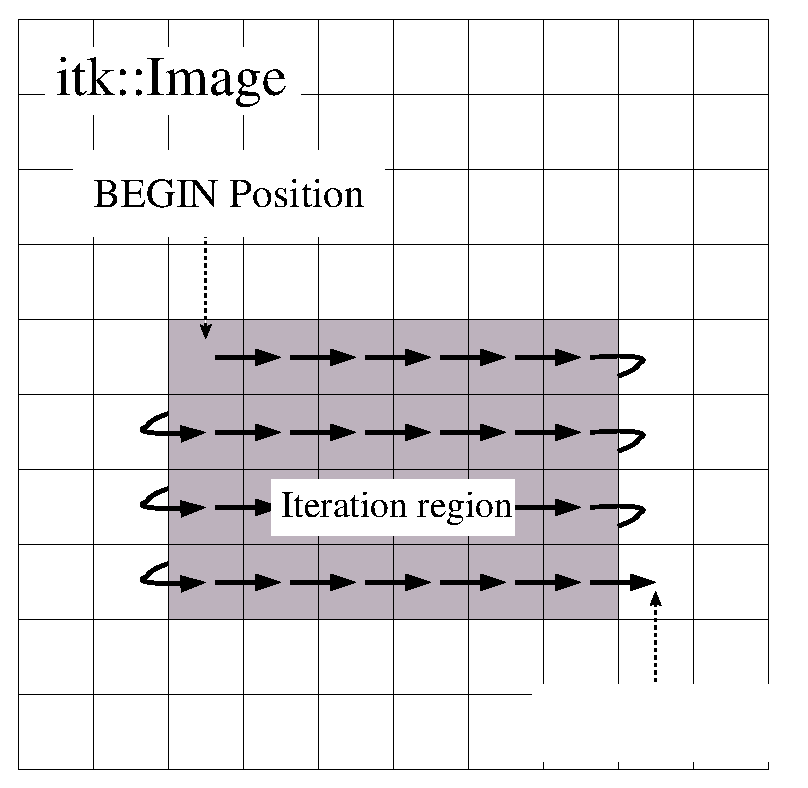
\includegraphics[width=0.4\textwidth]{IteratorFigure1.eps}
\itkcaption[ITK image iteration]{Normal path of an iterator through a
2D image.  The iteration region is shown in a darker shade.  An arrow denotes
a single iterator step, the result of one \code{++} operation.}
\protect\label{fig:WalkingIterator}
\end{figure}

In addition to sequential iteration through the image, some iterators may define
random access operators.  Unlike the increment operators, random access
operators may not be optimized for speed and require some knowledge of the
dimensionality of the image and the extent of the iteration region to use properly.

\begin{itemize}
\index{Iterators!operator+=()}
\item \textbf{\code{operator+=( OffsetType )}} Moves the iterator to the pixel
position at the current index plus specified \doxygen{Offset}.

\index{Iterators!operator-=()}
\item \textbf{\code{operator-=( OffsetType )}} Moves the iterator to
the pixel position at the current index minus specified Offset.

\index{Iterators!SetPosition()}
\item \textbf{\code{SetPosition( IndexType )}} Moves the iterator to the given
\doxygen{Index} position.
\end{itemize}

The \code{SetPosition()} method may be extremely slow for more complicated
iterator types. In general, it should only be used for setting a starting
iteration position, like you would use \code{GoToBegin()} or \code{GoToEnd()}.

Some iterators do not follow a predictable path through their
iteration regions and have no fixed beginning or ending pixel
locations.  A conditional iterator, for example, visits pixels only if
they have certain values or connectivities.  Random iterators,
increment and decrement to random locations and may even visit a given
pixel location more than once.

%Testing for location
An iterator can be queried to determine if it is at the end or the beginning of
its iteration region.

\begin{itemize}
\index{Iterators!IsAtEnd()}
\item \textbf{\code{bool IsAtEnd()}} True if the iterator points to \emph{one
position past} the end of the iteration region.

\index{Iterators!IsAtBegin()}
\item \textbf{\code{bool IsAtBegin()}} True if the iterator points to the first
position in the iteration region.  The method is typically used to test for the
end of reverse iteration.

\end{itemize}

An iterator can also report its current image index position.

\begin{itemize}
\index{Iterators!GetIndex()}
\item \textbf{\code{IndexType GetIndex()}} Returns the Index
of the image pixel that the iterator currently points to.
\end{itemize}

% A note on bounds checking
\index{Iterators!and bounds checking}
For efficiency, most ITK image iterators do not perform bounds checking.  It is
possible to move an iterator outside of its valid iteration region.
Dereferencing an out-of-bounds iterator will produce undefined results.

\subsection{Accessing Data}
\label{sec:AccessingData}
ITK image iterators define two basic methods for reading and writing pixel
values.

\begin{itemize}
\index{Iterators!Get()}
\item \textbf{\code{PixelType Get()}} Returns the value of the pixel at the
iterator position.

\index{Iterators!Set()}
\item \textbf{\code{void Set( PixelType )}} Sets the value of the pixel at the
iterator position.  Not defined for const versions of iterators.
\end{itemize}

% Describe efficiency due to inlining for all cases
The \code{Get()} and \code{Set()} methods are inlined and optimized
for speed so that their use is equivalent to dereferencing the image
buffer directly.  There are a few common cases, however, where using
\code{Get()} and \code{Set()} do incur a penalty. Consider the
following code, which fetches, modifies, and then writes a value back
to the same pixel location.

\small
\begin{verbatim}
  it.Set( it.Get() + 1 );
\end{verbatim}
\normalsize

As written, this code requires one more memory dereference than is necessary.
Some iterators define a third data access method that avoids this penalty.

\begin{itemize}
\index{Iterators!Value()}
\item \textbf{\code{PixelType \& Value()}} Returns a reference to the pixel at
the iterator position.
\end{itemize}

The \code{Value()} method can be used as either an lval or an rval in an
expression.  It has all the properties of \code{operator*}.  The
\code{Value()} method makes it possible to rewrite our example code more
efficiently.

\small
\begin{verbatim}
  it.Value()++;
\end{verbatim}
\normalsize

Consider using the \code{Value()} method instead of \code{Get()} or
\code{Set()} when a call to \code{operator=} on a pixel is non-trivial, such as
when working with vector pixels, and operations are done in-place in the
image. The disadvantage of using \code{Value} is that it cannot support image
adapters (see Section~\ref{sec:ImageAdaptors} on
page~\pageref{sec:ImageAdaptors} for more information about image adaptors).

\subsection{Iteration Loops}
\label{sec:IterationExample}
% Now give a psuedo code example for putting all of this together.
Using the methods described in the previous sections, we can now write a simple
example to do pixel-wise operations on an image.  The following code calculates
the squares of all values in an input image and writes them to an output image.

\small
\begin{verbatim}
  ConstIteratorType in( inputImage,   inputImage->GetRequestedRegion() );
  IteratorType out( outputImage, inputImage->GetRequestedRegion() );

  for ( in.GoToBegin(), out.GoToBegin(); !in.IsAtEnd(); ++in, ++out )
    {
    out.Set( in.Get() * in.Get() );
    }
\end{verbatim}
\normalsize

\index{Iterators!and image regions}
Notice that both the input and output iterators are initialized over the same
region, the \code{RequestedRegion} of \code{inputImage}.  This is good
practice because it ensures that the output iterator walks exactly the same set
of pixel indices as the input iterator, but does not require that the output
and input be the same size. The only requirement is that the input image
must contain a region (a starting index and size) that matches the
\code{RequestedRegion} of the output image.

\index{reverse iteration}
Equivalent code can be written by iterating through the image in reverse.
The syntax is slightly more awkward because the \emph{end} of the
iteration region is not a valid position and we can only test whether the
iterator is strictly \emph{equal} to its beginning position.  It is often more
convenient to write reverse iteration in a \code{while} loop.

\small
\begin{verbatim}
  in.GoToEnd();
  out.GoToEnd();
  while ( ! in.IsAtBegin() )
    {
    --in;
    --out;
    out.Set( in.Get() * in.Get() );
    }
\end{verbatim}
\normalsize

%\begin{itemize}
%\item \textbf{\code{operator==}}
%\item \textbf{\code{operator<}}
%\item \textbf{\code{operator<=}}
%\item \textbf{\code{operator>}}
%\item \textbf{\code{operator>=}}
%\end{itemize}

%operator +=, -=, etc

% SetIndex()

% operator <, operator >, etc.

\index{Iterators!programming interface|)}
\section{Image Iterators}
\label{sec:ImageIterators}
%Introduction and overview
This section describes iterators that walk rectilinear image regions and
reference a single pixel at a time.  The \doxygen{ImageRegionIterator} is the
most basic ITK image iterator and the first choice for most applications. The
rest of the iterators in this section are specializations of
ImageRegionIterator that are designed make common image processing
tasks more efficient or easier to implement.

% Each of the iterators has a const and non-const version

\subsection{ImageRegionIterator}
\index{itk::ImageRegionIterator|(}
\label{sec:itkImageRegionIterator}
\input{ImageRegionIterator.tex}
\index{itk::ImageRegionIterator|)}

\subsection{ImageRegionIteratorWithIndex}
\label{sec:itkImageRegionIteratorWithIndex}
\index{itk::ImageRegionIteratorWithIndex|(}
\input{ImageRegionIteratorWithIndex.tex}
\index{itk::ImageRegionIteratorWithIndex|)}

\subsection{ImageLinearIteratorWithIndex}
\label{sec:itkImageLinearIteratorWithIndex}
\index{itk::ImageLinearIteratorWithIndex|(}
\input{ImageLinearIteratorWithIndex.tex}
\input{ImageLinearIteratorWithIndex2.tex}
\index{itk::ImageLinearIteratorWithIndex|)}

\subsection{ImageSliceIteratorWithIndex}
\label{sec:itkImageSliceIteratorWithIndex}
\index{itk::ImageSliceIteratorWithIndex|(}
\input{ImageSliceIteratorWithIndex.tex}
\index{itk::ImageSliceIteratorWithIndex|)}

\subsection{ImageRandomConstIteratorWithIndex}
\label{sec:itkImageRandomConstIteratorWithIndex}
\index{itk::Image\-Random\-Const\-Iterator\-With\-Index|(}
\input{ImageRandomConstIteratorWithIndex}
\index{itk::Image\-Random\-Const\-Iterator\-With\-Index|)}

%\section{Conditional Iterators}
%\index{Iterators!conditional|(}
%\label{sec:ConditionalIterators}
%This section describes iterators that walk only pixels in an image region whose
%values satisfy a specified condition.  The condition is usually based on some
%function of the image values, such as comparing to a threshold.  When the
%condition function returns \code{true} at a pixel location, the iterator
%includes that location in its path.  The biggest use of these iterators is for
%walking non-rectilinear regions of interest, such as might be defined by
%implicit geometric shape functions or connected component regions.

%./Common/itkConditionalConstIterator.h (BaseClass)
%./Common/itkConditionalIterator.h (BaseClass)
%./Common/itkFloodFilledFunctionConditionalConstIterator.h (BaseClass)
%./Common/itkFloodFilledFunctionConditionalIterator.h (BaseClass)

%[ here are all classes where these filters are used:
% ./BasicFilters/itkConfidenceConnectedImageFilter.hxx (ImageFunction)
% ./BasicFilters/itkConnectedThresholdImageFilter.hxx (ImageFunction)
% ./BasicFilters/itkIsolatedConnectedImageFilter.hxx (ImageFunction)
% ./BasicFilters/itkNeighborhoodConnectedImageFilter.hxx (ImageFunction)
%
% ./Common/itkBinaryBallStructuringElement.hxx (SpatialFunction)
% ./Common/itkBloxCoreAtomImage.hxx (SpatialFunction)
% ./BasicFilters/itkBloxBoundaryPointToCoreAtomImageFilter.hxx (SpatialFunction)
% ./BasicFilters/itkBloxBoundaryPointImageToBloxBoundaryProfileImageFilter.hxx (SpatialFunction)
%]

%\subsection{itk::FloodFilledImageFunctionConditionalIterator}
%\label{itk::FloodFilledImageFunctionConditionalIterator}
%\index{itk::FloodFilledImageFunctionConditionalIterator|(}
%./Common/itkFloodFilledImageFunctionConditionalConstIterator.h
%./Common/itkFloodFilledImageFunctionConditionalIterator.h
%\index{itk::FloodFilledImageFunctionConditionalIterator|)}

%\subsection{itk::FloodFilledSpatialFunctionConditionalIterator}
%\label{itk::FloodFilledSpatialFunctionConditionalIterator}
%\index{itk::FloodFilledSpatialFunctionConditionalIterator|(}
%./Common/itkFloodFilledSpatialFunctionConditionalConstIterator.h
%./Common/itkFloodFilledSpatialFunctionConditionalIterator.h
%\index{itk::FloodFilledImageFunctionConditionalIterator|)}
%\index{Iterators!conditional|)}

\section{Neighborhood Iterators}
\label{sec:NeighborhoodIterators}
\index{Iterators!neighborhood|(}
In ITK, a pixel neighborhood is loosely defined as a small set of pixels that
are locally adjacent to one another in an image.  The size and shape
of a neighborhood, as well the connectivity among pixels in a neighborhood,
may vary with the application.

Many image processing algorithms are neighborhood-based, that is, the result at
a pixel $i$ is computed from the values of pixels in the ND neighborhood of
$i$. Consider finite difference operations in 2D.  A derivative at pixel index
$i = (j, k)$, for example, is taken as a weighted difference of the values
at $(j+1, k)$ and $(j-1, k)$. Other common examples of neighborhood operations
include convolution filtering and image morphology.

This section describes a class of ITK image iterators that are designed for
working with pixel neighborhoods. An ITK neighborhood iterator walks an image
region just like a normal image iterator, but instead of only referencing a
single pixel at each step, it simultaneously points to the entire ND
neighborhood of pixels.  Extensions to the standard iterator interface provide
read and write access to all neighborhood pixels and information
such as the size, extent, and location of the neighborhood.

Neighborhood iterators use the same operators defined in
Section~\ref{sec:IteratorsInterface} and the same code constructs as normal
iterators for looping through an
image. Figure~\ref{fig:NeighborhoodIteratorFig1} shows a neighborhood iterator
moving through an iteration region.  This iterator defines a $3x3$ neighborhood
around each pixel that it visits. The \emph{center} of the neighborhood
iterator is always positioned over its current index and all other neighborhood
pixel indices are referenced as offsets from the center index.  The pixel
under the center of the neighborhood iterator and all pixels under the shaded
area, or \emph{extent}, of the iterator can be dereferenced.

\begin{figure}
\centering
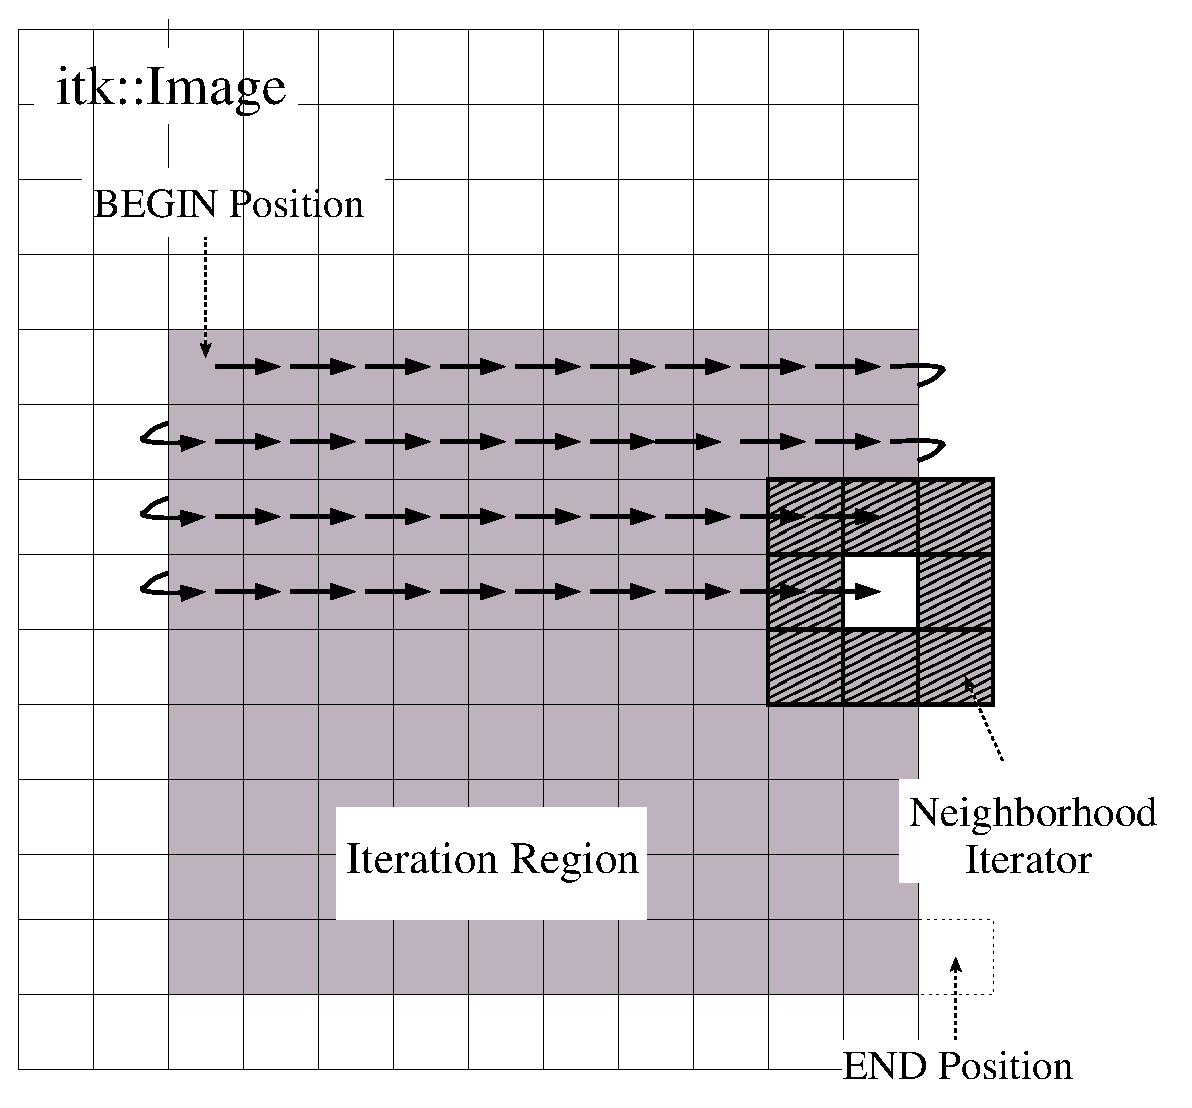
\includegraphics[width=0.6\textwidth]{NeighborhoodIteratorFig1.eps}
\itkcaption[Neighborhood iterator]{Path of a $3x3$ neighborhood
iterator through a 2D image region.  The extent of the neighborhood is
indicated by the hashing around the iterator position. Pixels that lie within
this extent are accessible through the iterator.  An arrow denotes a single
iterator step, the result of one \code{++} operation.}
\protect\label{fig:NeighborhoodIteratorFig1}
\end{figure}

\index{Neighborhood iterators!construction of}
\index{Neighborhood iterators!radius of}

In addition to the standard image pointer and iteration region
(Section~\ref{sec:IteratorsInterface}), neighborhood iterator constructors
require an argument that specifies the extent of the neighborhood to cover.
Neighborhood extent is symmetric across its center in each
axis and is given as an array of $N$ distances that are collectively called the
\emph{radius}. Each element $d$ of the radius, where $0 < d < N$ and
$N$ is the dimensionality of the neighborhood, gives the extent of the
neighborhood in pixels for dimension $N$.  The length of each face of the
resulting ND hypercube is $2d + 1$ pixels, a distance of $d$ on either side of
the single pixel at the neighbor center.
Figure~{\ref{fig:NeighborhoodIteratorFig2} shows the relationship between the
radius of the iterator and the size of the neighborhood for a variety of 2D
iterator shapes.

The radius of the neighborhood iterator is queried after construction
by calling the \code{GetRadius()} method.  Some other methods provide
some useful information about the iterator and its underlying image.

\begin{figure}
\centering
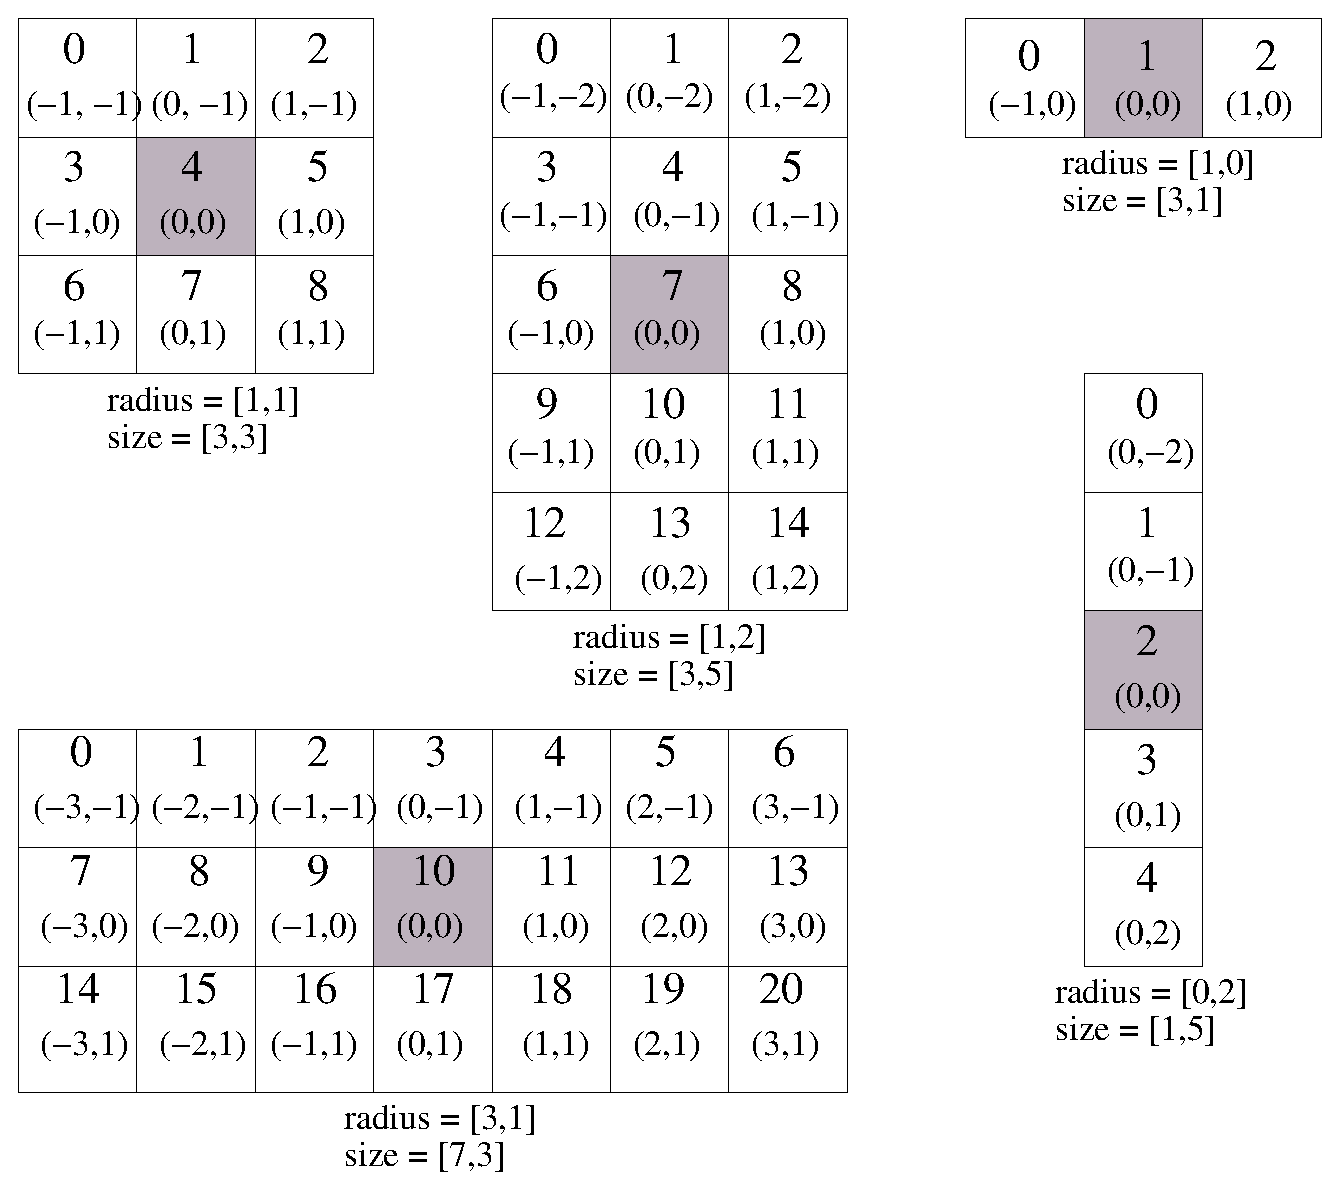
\includegraphics[width=0.9\textwidth]{NeighborhoodIteratorFig2.eps}
\itkcaption[Some possible neighborhood iterator shapes]{Several possible 2D
neighborhood iterator shapes are shown along with their radii and sizes.  A
neighborhood pixel can be dereferenced by its integer index (top) or its
offset from the center (bottom).  The center pixel of each iterator is
shaded.}
\protect\label{fig:NeighborhoodIteratorFig2}
\end{figure}

\begin{itemize}

\index{NeighborhoodIterator!GetRadius()}
\item \textbf{\code{SizeType GetRadius()}} Returns the ND radius of the
neighborhood as an \doxygen{Size}.

\index{NeighborhoodIterator!GetImagePointer()}
\item \textbf{\code{const ImageType *GetImagePointer()}} Returns the pointer to
the image referenced by the iterator.

\index{NeighborhoodIterator!Size()}
\item \textbf{\code{unsigned long Size()}} Returns the size in number of
pixels of the neighborhood.

\end{itemize}

The neighborhood iterator interface extends the normal ITK iterator interface
for setting and getting pixel values.  One way to dereference pixels is to
think of the neighborhood as a linear array where each pixel has a unique
integer index. The index of a pixel in the array is determined by incrementing
from the upper-left-forward corner of the neighborhood along the fastest
increasing image dimension: first column, then row, then slice, and so on.  In
Figure~\ref{fig:NeighborhoodIteratorFig2}, the unique integer index is shown
at the top of each pixel.  The center pixel is always at position $n/2$, where
$n$ is the size of the array.

\begin{itemize}

\index{NeighborhoodIterator!GetPixel()}
\item \textbf{\code{PixelType GetPixel(const unsigned int i)}} Returns the
value of the pixel at neighborhood position \code{i}.

\index{NeighborhoodIterator!SetPixel()}
\item \textbf{\code{void SetPixel(const unsigned int i, PixelType p)}}
Sets the value of the pixel at position \code{i} to \code{p}.

\end{itemize}

Another way to think about a pixel location in a neighborhood is as an
ND offset from the neighborhood center.  The upper-left-forward corner
of a $3x3x3$ neighborhood, for example, can be described by offset
$(-1, -1, -1)$.  The bottom-right-back corner of the same neighborhood
is at offset $(1, 1, 1)$.  In
Figure~\ref{fig:NeighborhoodIteratorFig2}, the offset from center is
shown at the bottom of each neighborhood pixel.

\begin{itemize}

\index{NeighborhoodIterator!GetPixel()}
\item \textbf{\code{PixelType GetPixel(const OffsetType \&o)}} Get the value of
the pixel at the position offset \code{o} from the neighborhood center.

\index{NeighborhoodIterator!SetPixel()}
\item \textbf{\code{void SetPixel(const OffsetType \&o, PixelType p)}} Set
the value at the position offset \code{o} from the neighborhood center to
the value \code{p}.

\end{itemize}

The neighborhood iterators also provide a shorthand for setting and getting the
value at the center of the neighborhood.

\index{NeighborhoodIterators!}
\begin{itemize}

\index{NeighborhoodIterator!GetCenterPixel()}
\item \textbf{\code{PixelType GetCenterPixel()}} Gets the value at the center
of the neighborhood.

\index{NeighborhoodIterator!SetCenterPixel()}
\item \textbf{\code{void SetCenterPixel(PixelType p)}} Sets the value at the
center of the neighborhood to the value \code{p}

\end{itemize}

There is another shorthand for setting and getting values for pixels that
lie some integer distance from the neighborhood center along one of the image
axes.

\index{NeighborhoodIterators!}
\begin{itemize}

\index{NeighborhoodIterator!GetNext()}
\item \textbf{\code{PixelType GetNext(unsigned int d)}} Get the value
immediately adjacent to the neighborhood center in the positive direction along
the \code{d} axis.

\index{NeighborhoodIterator!SetNext()}
\item \textbf{\code{void SetNext(unsigned int d, PixelType p)}} Set the value
immediately adjacent to the neighborhood center in the positive direction along
the \code{d} axis to the value \code{p}.

\index{NeighborhoodIterator!GetPrevious()}
\item \textbf{\code{PixelType GetPrevious(unsigned int d)}} Get the value
immediately adjacent to the neighborhood center in the negative direction along
the \code{d} axis.

\index{NeighborhoodIterator!SetPrevious()}
\item \textbf{\code{void SetPrevious(unsigned int d, PixelType p)}}
Set the value immediately adjacent to the neighborhood center in the
negative direction along the \code{d} axis to the value \code{p}.

\item \textbf{\code{PixelType GetNext(unsigned int d, unsigned int
s)}} Get the value of the pixel located \code{s} pixels from the
neighborhood center in the positive direction along the \code{d} axis.

\item \textbf{\code{void SetNext(unsigned int d, unsigned int s, PixelType p)}}
Set the value of the pixel located \code{s} pixels from the neighborhood center
in the positive direction along the \code{d} axis to value \code{p}.

\item \textbf{\code{PixelType GetPrevious(unsigned int d, unsigned int
s)}} Get the value of the pixel located \code{s} pixels from the
neighborhood center in the positive direction along the \code{d} axis.

\item \textbf{\code{void SetPrevious(unsigned int d, unsigned int s,
PixelType p)}} Set the value of the pixel located \code{s} pixels from
the neighborhood center in the positive direction along the \code{d}
axis to value \code{p}.

\end{itemize}

It is also possible to extract or set all of the neighborhood values
from an iterator at once using a regular ITK neighborhood object.
This may be useful in algorithms that perform a particularly large
number of calculations in the neighborhood and would otherwise require
multiple dereferences of the same pixels.

\begin{itemize}

\index{NeighborhoodIterator!GetNeighborhood()}
\index{NeighborhoodIterator!SetNeighborhood()}
\item \textbf{\code{NeighborhoodType GetNeighborhood()}} Return a
\doxygen{Neighborhood} of the same size and shape as the neighborhood
iterator and contains all of the values at the iterator position.

\item \textbf{\code{void SetNeighborhood(NeighborhoodType \&N)}} Set all
of the values in the neighborhood at the iterator position to those contained
in Neighborhood \code{N}, which must be the same size and shape as the
iterator.

\end{itemize}

Several methods are defined to provide information about the neighborhood.

\index{NeighborhoodIterators!}
\begin{itemize}

\index{NeighborhoodIterator!GetIndex()}
\item \textbf{\code{IndexType GetIndex()}} Return the image
index of the center pixel of the neighborhood iterator.

\item \textbf{\code{IndexType GetIndex(OffsetType o)}} Return the
image index of the pixel at offset \code{o} from the neighborhood
center.

\item \textbf{\code{IndexType GetIndex(unsigned int i)}} Return the
image index of the pixel at array position \code{i}.

\index{NeighborhoodIterator!GetOffset()}
\item \textbf{\code{OffsetType GetOffset(unsigned int i)}}  Return the offset
from the neighborhood center of the pixel at array position \code{i}.

\index{NeighborhoodIterator!GetNeighborhoodIndex()}
\item \textbf{\code{unsigned long GetNeighborhoodIndex(OffsetType o)}}
Return the array position of the pixel at offset \code{o} from the
neighborhood center.

\index{NeighborhoodIterator!GetSlice()}
\item \textbf{\code{std::slice GetSlice(unsigned int n)}} Return a
\code{std::slice} through the iterator neighborhood along axis \code{n}.

\end{itemize}

\index{Neighborhood iterators!boundary conditions}
\index{Neighborhood iterators!bounds checking}
A neighborhood-based calculation in a neighborhood close to an image
boundary may require data that falls outside the boundary.  The
iterator in Figure~\ref{fig:NeighborhoodIteratorFig1}, for example, is
centered on a boundary pixel such that three of its neighbors actually
do not exist in the image.  When the extent of a neighborhood falls
outside the image, pixel values for missing neighbors are supplied
according to a rule, usually chosen to satisfy the numerical
requirements of the algorithm.  A rule for supplying out-of-bounds
values is called a \emph{boundary condition}.

ITK neighborhood iterators automatically detect out-of-bounds dereferences and
will return values according to boundary conditions.  The boundary condition
type is specified by the second, optional template parameter of the iterator.
By default, neighborhood iterators use a Neumann condition where the first
derivative across the boundary is zero.  The Neumann rule simply returns the
closest in-bounds pixel value to the requested out-of-bounds location.  Several
other common boundary conditions can be found in the ITK toolkit.  They include
a periodic condition that returns the pixel value from the opposite side of the
data set, and is useful when working with periodic data such as Fourier
transforms, and a constant value condition that returns a set value $v$ for all
out-of-bounds pixel dereferences.  The constant value condition is equivalent
to padding the image with value $v$.

Bounds checking is a computationally expensive operation because it occurs each
time the iterator is incremented.  To increase efficiency, a neighborhood
iterator automatically disables bounds checking when it detects that it is
not necessary.  A user may also explicitly disable or enable bounds checking.
Most neighborhood based algorithms can minimize the need for bounds checking
through clever definition of iteration regions.  These techniques are explored
in Section~\ref{sec:NeighborhoodExample3}.

\begin{itemize}

\index{NeighborhoodIterator!NeedToUseBoundaryConditionOn()}
\item \textbf{\code{void NeedToUseBoundaryConditionOn()}} Explicitly turn
bounds checking on.  This method should be used with caution because
unnecessarily enabling bounds checking may result in a significant performance
decrease. In general you should allow the iterator to automatically determine
this setting.

\index{NeighborhoodIterator!NeedToUseBoundaryConditionOff()}
\item \textbf{\code{void NeedToUseBoundaryConditionOff()}} Explicitly disable
bounds checking. This method should be used with caution because disabling
bounds checking when it is needed will result in out-of-bounds reads and
undefined results.

\index{NeighborhoodIterator!OverrideBoundaryCondition()}
\item \textbf{\code{void OverrideBoundaryCondition(BoundaryConditionType *b)}}
Overrides the templated boundary condition, using boundary condition
object \code{b} instead. Object \code{b} should not be deleted until
it has been released by the iterator.  This method can be used to
change iterator behavior at run-time.

\index{NeighborhoodIterator!ResetBoundaryCondition()}
\item \textbf{\code{void ResetBoundaryCondition()}} Discontinues the use of any
run-time specified boundary condition and returns to using the condition
specified in the template argument.

\index{NeighborhoodIterator!SetPixel()}
\item \textbf{\code{void SetPixel(unsigned int i, PixelType p, bool
status)}} Sets the value at neighborhood array position \code{i} to value
\code{p}.  If the position \code{i} is out-of-bounds, \code{status} is set to
\code{false}, otherwise \code{status} is set to \code{true}.
\end{itemize}

The following sections describe the two ITK neighborhood iterator classes,
\doxygen{NeighborhoodIterator} and \doxygen{ShapedNeighborhoodIterator}.
Each has a const and a non-const version.  The shaped iterator is a refinement
of the standard NeighborhoodIterator that supports an
arbitrarily-shaped (non-rectilinear) neighborhood.

\subsection{NeighborhoodIterator}
\label{sec:itkNeighborhoodIterator}

\index{NeighborhoodIterator!examples}
\index{Neighborhood iterators!examples}
The standard neighborhood iterator class in ITK is the
\doxygen{NeighborhoodIterator}.  Together with its \code{const} version,
\doxygen{ConstNeighborhoodIterator}, it implements the complete API
described above.  This section provides several examples to illustrate the use
of NeighborhoodIterator.

\index{edge detection}
\index{Sobel operator}
\subsubsection{Basic neighborhood techniques: edge detection}
\label{sec:NeighborhoodExample1}
\input{NeighborhoodIterators1.tex}

\index{convolution filtering}
\index{Sobel operator}
\subsubsection{Convolution filtering: Sobel operator}
\label{sec:NeighborhoodExample2}
\input{NeighborhoodIterators2.tex}

\subsubsection{Optimizing iteration speed}
\label{sec:NeighborhoodExample3}
\input{NeighborhoodIterators3.tex}

\index{Gaussian blurring}
\subsubsection{Separable convolution: Gaussian filtering}
\label{sec:NeighborhoodExample4}
\input{NeighborhoodIterators4.tex}

\subsubsection{Slicing the neighborhood}
\label{sec:NeighborhoodExample5}
\input{NeighborhoodIterators5.tex}

\subsubsection{Random access iteration}
\label{sec:NeighborhoodExample6}
\input{NeighborhoodIterators6.tex}

%./Common/itkConstNeighborhoodIterator.h
%./Common/itkNeighborhoodIterator.h

% Example1: Edge detection using ``hand-coded'' Sobel operator
% Example2: Sobel edge detection using convolution filtering and Sobel operator
% Example3: Improving boundary condition efficiency
% Example4: gaussian filtering, separable convolution
% Example5: Slicing the neighborhood: gaussian filtering, separable convolution
% Example6: Advanced Neighborhood Techniques: local minima, local maxima

\subsection{ShapedNeighborhoodIterator}
\label{sec:itkShapedNeighborhoodIterator}
\index{ShapedNeighborhoodIterator}
\index{Neighborhood iterators!shaped}
\index{Neighborhood iterators!as stencils}
This section describes a variation on the neighborhood iterator called a
\emph{shaped} neighborhood iterator.  A shaped neighborhood is defined like
a bit mask, or \emph{stencil}, with different offsets in the rectilinear
neighborhood of the normal neighborhood iterator turned off or on to create a
pattern.  Inactive positions (those not in the stencil) are not updated during
iteration and their values cannot be read or written.  The shaped iterator is
implemented in the class \doxygen{ShapedNeighborhoodIterator}, which is a
subclass of
\doxygen{NeighborhoodIterator}.  A const version,
\doxygen{ConstShapedNeighborhoodIterator}, is also available.

\index{Neighborhood iterators!active neighbors}
\index{Neighborhood iterators!inactive neighbors}
Like a regular neighborhood iterator, a shaped neighborhood iterator must be
initialized with an ND radius object, but the radius of the neighborhood of a
shaped iterator only defines the set of \emph{possible} neighbors.  Any number
of possible neighbors can then be activated or deactivated.  The shaped
neighborhood iterator defines an API for activating neighbors.  When a neighbor
location, defined relative to the center of the neighborhood, is activated, it
is placed on the \emph{active list} and is then part of the stencil.  An
iterator can be ``reshaped'' at any time by adding or removing offsets from the
active list.

\begin{itemize}

\index{ShapedNeighborhoodIterator!ActivateOffset()}
\item \textbf{\code{void ActivateOffset(OffsetType \&o)}} Include the offset
\code{o} in the stencil of active neighborhood positions.  Offsets are relative
to the neighborhood center.

\index{ShapedNeighborhoodIterator!DeactivateOffset()}
\item \textbf{\code{void DeactivateOffset(OffsetType \&o)}} Remove the offset
\code{o} from the stencil of active neighborhood positions.  Offsets are
relative to the neighborhood center.

\index{ShapedNeighborhoodIterator!ClearActiveList()}
\item \textbf{\code{void ClearActiveList()}} Deactivate all positions in the
iterator stencil by clearing the active list.

\index{ShapedNeighborhoodIterator!GetActiveIndexListSize()}
\item \textbf{\code{unsigned int GetActiveIndexListSize()}} Return the number
of pixel locations that are currently active in the shaped iterator stencil.

\end{itemize}

Because the neighborhood is less rigidly defined in the shaped iterator, the
set of pixel access methods is restricted.  Only the \code{GetPixel()} and
\code{SetPixel()} methods are available, and calling these methods on an
inactive neighborhood offset will return undefined results.

For the common case of traversing all pixel offsets in a neighborhood, the
shaped iterator class provides an iterator through the active offsets in its
stencil.   This \emph{stencil iterator} can be incremented or decremented and
defines \code{Get()} and \code{Set()} for reading and writing the values in the
neighborhood.

\begin{itemize}
\index{ShapedNeighborhoodIterator!Iterator::Begin()}
\item \textbf{\code{ShapedNeighborhoodIterator::Iterator Begin()}} Return a
const or non-const iterator through the shaped iterator stencil that points to
the first valid location in the stencil.

\index{ShapedNeighborhoodIterator!Iterator::End()}
\item \textbf{\code{ShapedNeighborhoodIterator::Iterator End()}} Return a
const or non-const iterator through the shaped iterator stencil that points
\emph{one position past} the last valid location in the stencil.
\end{itemize}

The functionality and interface of the shaped neighborhood iterator is best
described by example.  We will use the ShapedNeighborhoodIterator to
implement some binary image morphology algorithms (see \cite{Gonzalez1993},
\cite{Castleman1996}, et al.).  The examples that follow implement erosion and
dilation.

\index{ShapedNeighborhoodIterator!examples of}
\subsubsection{Shaped neighborhoods: morphological operations}
\label{sec:ShapedNeighborhoodExample}
\input{ShapedNeighborhoodIterators1.tex}
\input{ShapedNeighborhoodIterators2.tex}

%./Common/itkConstShapedNeighborhoodIterator.h
%./Common/itkShapedNeighborhoodIterator.h

\index{Iterators!neighborhood|)}

% ADD A SECTION WITH TIPS, SUGGESTIONS ON USING ITERATORS?  EXTENDING ITERATORS?
% USING ITERATORS FOR MULTITHREADING EXAMPLE?
\index{Iterators!image|)}

  
\chapter{Image Adaptors}
\label{sec:ImageAdaptors}

\index{ImageAdaptors}

\begin{figure}
\center
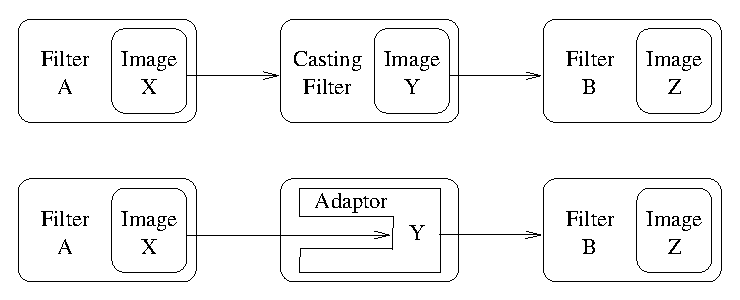
\includegraphics[width=0.8\textwidth]{ImageAdaptorConcept.eps}
\itkcaption[ImageAdaptor concept]{ The difference between using a
CastImageFilter and an ImageAdaptor.  ImageAdaptors
convert pixel values when they are accessed by iterators.  Thus, they do not
produces an intermediate image.  In the example
illustrated by this figure, the \emph{Image Y} is not created by the
ImageAdaptor; instead, the image is simulated on the fly each time an
iterator from the filter downstream attempts to access the image data.}
\label{fig:ImageAdaptorConcept}
\end{figure}

The purpose of an \emph{image adaptor} is to make one image appear
like another image, possibly of a different pixel type.  A typical
example is to take an image of pixel type \code{unsigned char} and
present it as an image of pixel type \code{float}. The motivation for
using image adaptors in this case is to avoid the extra memory
resources required by using a casting filter.  When we use the
\doxygen{CastImageFilter} for the conversion, the filter creates a
memory buffer large enough to store the \code{float} image. The
\code{float} image requires four times the memory of the
original image and contains no useful additional information. Image
adaptors, on the other hand, do not require the extra memory as
pixels are converted only when they are read using image iterators
(see Chapter~\ref{sec:ImageIteratorsChapter}).

Image adaptors are particularly useful when there is infrequent pixel access,
since the actual conversion occurs on the fly during the access operation. In
such cases the use of image adaptors may reduce overall computation time as
well as reduce memory usage. The use of image adaptors, however, can be
disadvantageous in some situations. For example, when the downstream filter
is executed multiple times, a CastImageFilter will cache its output after the
first execution and will not re-execute when the filter downstream is
updated. Conversely, an image adaptor will compute the cast every time.

Another application for image adaptors is to perform lightweight
pixel-wise operations replacing the need for a filter. In the toolkit,
adaptors are defined for many single valued and single parameter
functions such as trigonometric, exponential and logarithmic
functions. For example,
\begin{itemize}
\item \doxygen{ExpImageAdaptor}
\item \doxygen{SinImageAdaptor}
\item \doxygen{CosImageAdaptor}
\end{itemize}

The following examples illustrate common applications of image adaptors.

\section{Image Casting}
\label{sec:ImageAdaptorForBasicCasting}
\ifitkFullVersion
\input{ImageAdaptor1.tex}
\fi

\section{Adapting RGB Images}
\label{sec:ImageAdaptorForRGB}
\ifitkFullVersion
\input{ImageAdaptor2.tex}
\fi


\section{Adapting Vector Images}
\label{sec:ImageAdaptorForVectors}
\ifitkFullVersion
\input{ImageAdaptor3.tex}
\fi

\section{Adaptors for Simple Computation}
\label{sec:ImageAdaptorForSimpleComputation}
\ifitkFullVersion
\input{ImageAdaptor4.tex}
\fi


\section{Adaptors and Writers}

Image adaptors will not behave correctly when connected directly to a writer.
The reason is that writers tend to get direct access to the image buffer from
their input, since image adaptors do not have a real buffer their behavior in
this circumstances is incorrect. You should avoid instantiating the
\code{ImageFileWriter} or the \code{ImageSeriesWriter} over an image adaptor
type.


  \chapter{How To Write A Filter}
\label{chapter:WriteAFilter}

This purpose of this chapter is help developers create their own
filter (process object).  This chapter is divided into four major
parts. An initial definition of terms is followed by an overview of
the filter creation process. Next, data streaming is discussed. The
way data is streamed in ITK must be understood in order to write
correct filters. Finally, a section on multithreading describes what
you must do in order to take advantage of shared memory parallel
processing.

\section{Terminology}
\label{sec:Terminology}

The following is some basic terminology for the discussion that follows.
Chapter \ref{chapter:SystemOverview} provides additional background
information.

\begin{itemize}
        \item The \textbf{data processing pipeline} is a directed graph of
        \textbf{process} and \textbf{data objects}. The pipeline inputs,
        operators on, and outputs data.
        \index{data processing pipeline}
        \index{process object}
        \index{data object}

        \item A \textbf{filter}, or \textbf{process object}, has one or more
        inputs, and one or more outputs.
        \index{filter}

        \item A \textbf{source}, or source process object, initiates the data
        processing pipeline, and has one or more outputs.
        \index{source}

        \item A \textbf{mapper}, or mapper process object, terminates the
        data processing pipeline. The mapper has one or more outputs, and may
        write data to disk, interface with a display system, or interface to
        any other system.
        \index{mapper}

        \item A \textbf{data object} represents and provides access to
        data. In ITK, the data object (ITK class \doxygen{DataObject}) is
        typically of type \doxygen{Image} or \doxygen{Mesh}.
        \index{data object}

        \item A \textbf{region} (ITK class \doxygen{Region}) represents a
        piece, or subset of the entire data set.
        \index{region}

        \item An \textbf{image region} (ITK class \doxygen{ImageRegion})
        represents a structured portion of data. ImageRegion is implemented
        using the \doxygen{Index} and \doxygen{Size} classes
        \index{image region}

        \item A \textbf{mesh region} (ITK class \doxygen{MeshRegion})
        represents an unstructured portion of data.
        \index{mesh region}

        \item The \textbf{LargestPossibleRegion} is the theoretical single,
        largest piece (region) that could represent the entire dataset. The
        LargestPossibleRegion is used in the system as the measure of the
        largest possible data size.
        \index{LargestPossibleRegion}

        \item The \textbf{BufferedRegion} is a contiguous block of memory
        that is less than or equal to in size to the
        LargestPossibleRegion. The buffered region is what has actually been
        allocated by a filter to hold its output.
        \index{BufferedRegion}

        \item The \textbf{RequestedRegion} is the piece of the dataset that a
        filter is required to produce. The RequestedRegion is less than or
        equal in size to the BufferedRegion. The RequestedRegion may differ
        in size from the BufferedRegion due to performance reasons. The
        RequestedRegion may be set by a user, or by an application that needs
        just a portion of the data.
        \index{RequestedRegion}

        \item The \textbf{modified time} (represented by ITK class
        \doxygen{TimeStamp}) is a monotonically increasing integer value that
        characterizes a point in time when an object was last modified.
        \index{modified time}

        \item \textbf{Downstream} is the direction of dataflow, from sources
        to mappers.
        \index{pipeline!downstream}

        \item \textbf{Upstream} is the opposite of downstream, from mappers
        to sources.
        \index{pipeline!upstream}

        \item The \textbf{pipeline modified time} for a particular data
        object is the maximum modified time of all upstream data objects and
        process objects.
        \index{pipeline!modified time}

        \item The term \textbf{information} refers to metadata that
        characterizes data. For example, index and dimensions are information
        characterizing an image region.
        \index{pipeline!information}
\end{itemize}

\section{Overview of Filter Creation}
\label{sec:OverviewFilterCreation}
\index{filter!overview of creation}

\begin{floatingfigure}[rlp]{7cm}
  \centering
  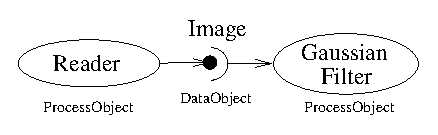
\includegraphics[width=6cm]{DataPipelineOneConnection.eps}
  \caption[Relationship between DataObjects and ProcessObjects]
{Relationship between DataObject and ProcessObject.
\label{fig:DataPipeLineOneConnection}}
\end{floatingfigure}


Filters are defined with respect to the type of data they input (if
any), and the type of data they output (if any). The key to writing a
ITK filter is to identify the number and types of input and
output. Having done so, there are often superclasses that simplify
this task via class derivation. For example, most filters in ITK take
a single image as input, and produce a single image on output. The
superclass \doxygen{ImageToImageFilter} is a convenience class that
provide most of the functionality needed for such a filter.

Some common base classes for new filters include:

\begin{itemize}

  \item \code{ImageToImageFilter}: the most common filter base for
    segmentation algorithms.  Takes an image and produces a new image, by
    default of the same dimensions.  Override
    \code{GenerateOutputInformation} to produce a different size.

  \item \code{UnaryFunctorImageFilter}: used when defining a filter that
  applies a function to an image.

  \item \code{BinaryFunctorImageFilter}: used when defining a filter that
  applies an operation to two images.

  \item \code{ImageFunction}: a functor that can be applied to an image,
  evaluating $f(x) $ at each point in the image.

  \item \code{MeshToMeshFilter}: a filter that transforms meshes, such as
  tessellation, polygon reduction, and so on.

  \item \code{LightObject}: abstract base for filters that don't fit well
  anywhere else in the class hierarchy.  Also useful for ``calculator''
  filters; ie. a sink filter that takes an input and calculates a result
  which is retrieved using a \code{Get()} method.

\end{itemize}

Once the appropriate superclass is identified, the filter writer
implements the class defining the methods required by most all ITK
objects: \code{New()}, \code{PrintSelf()}, and protected constructor,
copy constructor, delete, and operator=, and so on. Also, don't forget
standard typedefs like \code{Self}, \code{Superclass}, \code{Pointer}, and
\code{ConstPointer}. Then the filter writer can focus on the most important
parts of the implementation: defining the API, data members, and other
implementation details of the algorithm. In particular, the filter writer
will have to implement either a \code{GenerateData()} (non-threaded) or
\code{ThreadedGenerateData()} method. (See Section~\ref{sec:MultiThreading}
for an overview of multi-threading in ITK.)

An important note: the GenerateData() method is required to allocate memory
for the output. The ThreadedGenerateData() method is not. In default
implementation (see \doxygen{ImageSource}, a superclass of
\doxygen{ImageToImageFilter})
\code{GenerateData()} allocates memory and then invokes
\code{ThreadedGenerateData()}.

One of the most important decisions that the developer must make is whether
the filter can stream data; that is, process just a portion of the input to
produce a portion of the output. Often superclass behavior works well: if the
filter processes the input using single pixel access, then the default
behavior is adequate. If not, then the user may have to a) find a more
specialized superclass to derive from, or b) override one or more methods
that control how the filter operates during pipeline execution. The next
section describes these methods.



\section{Streaming Large Data}
\label{sec:StreamingLargeData}
\index{pipeline!streaming large data}

The data associated with multi-dimensional images is large and becoming larger.
This trend is due to advances in scanning resolution, as well as increases in
computing capability. Any practical segmentation and registration software
system must address this fact in order to be useful in application. ITK
addresses this problem via its data streaming facility.

In ITK, streaming is the process of dividing data into pieces, or regions,
and then processing this data through the data pipeline. Recall that the
pipeline consists of process objects that generate data objects, connected
into a pipeline topology. The input to a process object is a data object
(unless the process initiates the pipeline and then it is a source process
object). These data objects in turn are consumed by other process objects,
and so on, until a directed graph of data flow is constructed. Eventually the
pipeline is terminated by one or more mappers, that may write data to
storage, or interface with a graphics or other system. This is illustrated in
figures \ref{fig:DataPipeLineOneConnection} and \ref{fig:DataPipeLine}.

A significant benefit of this architecture is that the relatively complex
process of managing pipeline execution is designed into the system. This
means that keeping the pipeline up to date, executing only those portions of
the pipeline that have changed, multithreading execution, managing memory
allocation, and streaming is all built into the architecture. However, these
features do introduce complexity into the system, the bulk of which is seen
by class developers. The purpose of this chapter is to describe the pipeline
execution process in detail, with a focus on data streaming.


\subsection{Overview of Pipeline Execution}
\label{sec:OverviewPipelineExecution}
\index{pipeline!overview of execution}

The pipeline execution process performs several important functions.

\begin{figure}
  \par\centering
  \resizebox{5in}{!}{ 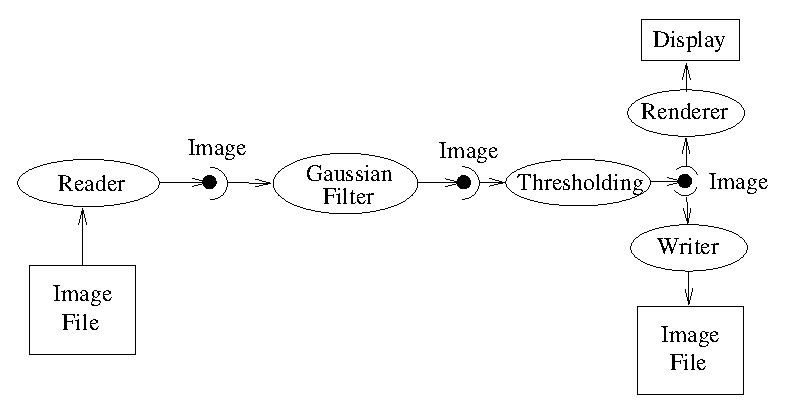
\includegraphics{DataPipeline.eps}}
  \itkcaption[The Data Pipeline]{The Data Pipeline}
  \label{fig:DataPipeLine}
  \par
\end{figure}

\begin{enumerate}
        \item It determines which filters, in a pipeline of filters, need to
        execute. This prevents redundant execution and minimizes overall
        execution time.

        \item It initializes the (filter's) output data objects, preparing
        them for new data.  In addition, it determines how much memory each
        filter must allocate for its output, and allocates it.

        \item The execution process determines how much data a filter must
        process in order to produce an output of sufficient size for
        downstream filters; it also takes into account any limits on memory
        or special filter requirements. Other factors include the size of
        data processing kernels, that affect how much data input data
        (extra padding) is required.

        \item It subdivides data into subpieces for multithreading. (Note
        that the division of data into subpieces is exactly same problem as
        dividing data into pieces for streaming; hence multithreading comes
        for free as part of the streaming architecture.)

        \item It may free (or release) output data if filters no longer need
        it to compute, and the user requests that data is to be
        released. (Note: a filter's output data object may be considered a
        ``cache''. If the cache is allowed to remain (\code{ReleaseDataFlagOff()})
        between pipeline execution, and the filter, or the input to the
        filter, never changes, then process objects downstream of the filter
        just reuse the filter's cache to re-execute.)
\end{enumerate}

To perform these functions, the execution process negotiates with the
filters that define the pipeline. Only each filter can know how much data is
required on input to produce a particular output. For example, a shrink
filter with a shrink factor of two requires an image twice as large (in terms
of its x-y dimensions) on input to produce a particular size output. An
image convolution filter would require extra input (boundary padding)
depending on the size of the convolution kernel. Some filters require the
entire input to produce an output (for example, a histogram), and have the
option of requesting the entire input. (In this case streaming does not work
unless the developer creates a filter that can request multiple pieces,
caching state between each piece to assemble the final output.)


\begin{figure}
  \par\centering
  \resizebox{5in}{!}{ 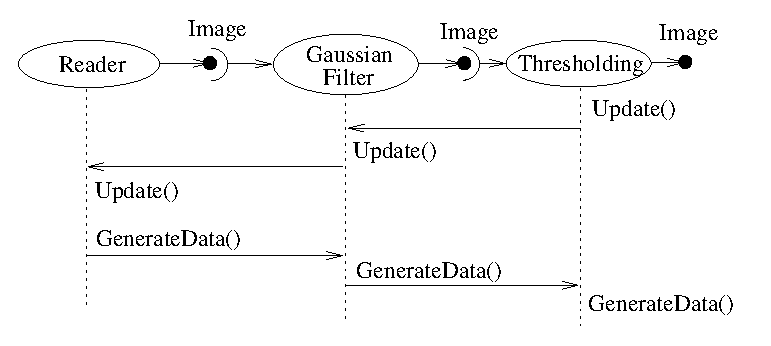
\includegraphics{DataPipelineUpdate.eps}}
  \itkcaption[Sequence of the Data Pipeline updating mechanism]{Sequence of the
Data Pipeline updating mechanism}
  \label{fig:DataPipeLineUpdate}
  \par
\end{figure}


Ultimately the negotiation process is controlled by the request for data of a
particular size (i.e., region). It may be that the user asks to process a
region of interest within a large image, or that memory limitations result in
processing the data in several pieces. For example, an application may
compute the memory required by a pipeline, and then use
\doxygen{StreamingImageFilter} to break the data processing into several pieces.
The data request is propagated through the pipeline in the upstream
direction, and the negotiation process configures each filter to produce
output data of a particular size.

The secret to creating a streaming filter is to understand how this
negotiation process works, and how to override its default behavior by using
the appropriate virtual functions defined in \doxygen{ProcessObject}. The next
section describes the specifics of these methods, and when to override
them. Examples are provided along the way to illustrate concepts.


\subsection{Details of Pipeline Execution}
\label{sec:DetailsPipelineExecution}
\index{pipeline!execution details}

Typically pipeline execution is initiated when a process object
receives the \code{ProcessObject::Update()} method invocation. This
method is simply delegated to the output of the filter, invoking the
\code{DataObject::Update()} method. Note that this behavior is typical
of the interaction between ProcessObject and DataObject: a method
invoked on one is eventually delegated to the other. In this way the
data request from the pipeline is propagated upstream, initiating data
flow that returns downstream.

The \code{DataObject::Update()} method in turn invokes three other methods:

\begin{itemize}
        \item \code{DataObject::UpdateOutputInformation()}
        \item \code{DataObject::PropagateRequestedRegion()}
        \item \code{DataObject::UpdateOutputData()}
\end{itemize}

\subsubsection{UpdateOutputInformation()}
\label{sec:UpdateOutputInformation}
\index{pipeline!UpdateOutputInformation}

The \code{UpdateOutputInformation()} method determines the pipeline modified
time. It may set the RequestedRegion and the LargestPossibleRegion depending
on how the filters are configured. (The RequestedRegion is set to process all
the data, i.e., the LargestPossibleRegion, if it has not been set.) The
UpdateOutputInformation() propagates upstream through the entire pipeline and
terminates at the sources.

During \code{UpdateOutputInformation()}, filters have a chance to override the
\code{ProcessObject::GenerateOutputInformation()} method
(\code{GenerateOutputInformation()} is invoked by
\code{UpdateOutputInformation()}). The default behavior is for the
\code{GenerateOutputInformation()} to copy the metadata describing the input
to the output (via \code{DataObject::CopyInformation()}). Remember, information
is metadata describing the output, such as the origin, spacing,
and LargestPossibleRegion (i.e., largest possible size) of an image.

A good example of this behavior is \doxygen{ShrinkImageFilter}. This filter
takes an input image and shrinks it by some integral value. The result is that
the spacing and LargestPossibleRegion of the output will be different to that
of the input. Thus, \code{GenerateOutputInformation()} is overloaded.

\subsubsection{PropagateRequestedRegion()}
\label{sec:PropagateRequestedRegion}
\index{pipeline!PropagateRequestedRegion}

The \code{PropagateRequestedRegion()} call propagates upstream to
satisfy a data request. In typical application this data request is usually the
LargestPossibleRegion, but if streaming is necessary, or the user is
interested in updating just a portion of the data, the RequestedRegion may be
any valid region within the LargestPossibleRegion.

The function of \code{PropagateRequestedRegion()} is, given a request
for data (the amount is specified by RequestedRegion), propagate
upstream configuring the filter's input and output process object's to
the correct size. Eventually, this means configuring the
BufferedRegion, that is the amount of data actually allocated.

The reason for the buffered region is this: the output of a filter may be
consumed by more than one downstream filter. If these consumers each request
different amounts of input (say due to kernel requirements or other padding
needs), then the upstream, generating filter produces the data to satisfy
both consumers, that may mean it produces more data than one of the
consumers needs.

The \code{ProcessObject::PropagateRequestedRegion()} method invokes
three methods that the filter developer may choose to overload.

\begin{itemize}
        \item \code{EnlargeOutputRequestedRegion(DataObject *output)} gives the
        (filter) subclass a chance to indicate that it will provide more data
        than required for the output. This can happen, for example, when a
        source can only produce the whole output (i.e., the
        LargestPossibleRegion).

        \item \code{GenerateOutputRequestedRegion(DataObject *output)} gives
        the subclass a chance to define how to set the requested regions for
        each of its outputs, given this output's requested region.  The default
        implementation is to make all the output requested regions the same.
        A subclass may need to override this method if each output is a
        different resolution. This method is only overridden if a filter has
        multiple outputs.

        \item \code{GenerateInputRequestedRegion()} gives the subclass a
        chance to
        request a larger requested region on the inputs. This is necessary
        when, for example, a filter requires more data at the ``internal''
        boundaries to produce the boundary values - due to kernel operations
        or other region boundary effects.
\end{itemize}

\doxygen{RGBGibbsPriorFilter} is an example of a filter that needs to
invoke \code{EnlargeOutputRequestedRegion()}. The designer of this
filter decided that the filter should operate on all the data. Note
that a subtle interplay between this method and
\code{GenerateInputRequestedRegion()} is occurring here. The default
behavior of \code{GenerateInputRequestedRegion()} (at least for
\doxygen{ImageToImageFilter}) is to set the input RequestedRegion to
the output's ReqestedRegion. Hence, by overriding the method
\code{EnlargeOutputRequestedRegion()} to set the output to the
LargestPossibleRegion, effectively sets the input to this filter to
the LargestPossibleRegion (and probably causing all upstream filters
to process their LargestPossibleRegion as well. This means that the
filter, and therefore the pipeline, does not stream. This could be
fixed by reimplementing the filter with the notion of streaming built
in to the algorithm.)

\doxygen{GradientMagnitudeImageFilter} is an example of a filter that needs to
invoke \code{GenerateInputRequestedRegion()}. It needs a larger input requested
region because a kernel is required to compute the gradient at a pixel. Hence
the input needs to be ``padded out'' so the filter has enough data to compute
the gradient at each output pixel.

\subsubsection{UpdateOutputData()}
\label{sec:UpdateOutputData}
\index{pipeline!UpdateOutputData}

\code{UpdateOutputData()} is the third and final method as a result of the
\code{Update()} method. The purpose of this method is to determine whether a
particular filter needs to execute in order to bring its output up to date. (A
filter executes when its \code{GenerateData()} method is invoked.) Filter
execution occurs when a) the filter is modified as a result of modifying an
instance variable; b) the input to the filter changes; c) the input data has
been released; or d) an invalid RequestedRegion was set previously and the
filter did not produce data. Filters execute in order in the downstream
direction.  Once a filter executes, all filters downstream of it must also
execute.

\code{DataObject::UpdateOutputData()} is delegated to the DataObject's source
(i.e., the ProcessObject that generated it) only if the DataObject needs to be
updated. A comparison of modified time, pipeline time, release data flag, and
valid requested region is made. If any one of these conditions indicate that
the data needs regeneration, then the source's
\code{ProcessObject::UpdateOutputData()} is invoked. These calls are made
recursively up the pipeline until a source filter object is encountered, or the
pipeline is determined to be up to date and valid. At this point, the recursion
unrolls, and the execution of the filter proceeds. (This means that the output
data is initialized, StartEvent is invoked, the filters \code{GenerateData()}
is called, EndEvent is invoked, and input data to this filter may be released,
if requested. In addition, this filter's InformationTime is updated to the
current time.)

The developer will never override \code{UpdateOutputData()}. The developer need
only write the \code{GenerateData()} method (non-threaded) or
\code{ThreadedGenerateData()} method. A discussion of threading follows in the
next section.


\section{Threaded Filter Execution}
\label{sec:ThreadedFilterExecution}
\index{pipeline!ThreadedFilterExecution}

Filters that can process data in pieces can typically multi-process
using the data parallel, shared memory implementation built into the
pipeline execution process. To create a multithreaded filter, simply
define and implement a \code{ThreadedGenerateData()} method. For
example, a \doxygen{ImageToImageFilter} would create the method:

\small
\begin{minted}[baselinestretch=1,fontsize=\footnotesize,linenos=false,bgcolor=ltgray]{cpp}
    virtual void ThreadedGenerateData( const OutputImageRegionType&
      outputRegionForThread, ThreadIdType threadId ) ITK_OVERRIDE;
\end{minted}
\normalsize

The key to threading is to generate output for the output region given (as
the first parameter in the argument list above). In ITK, this is simple to do
because an output iterator can be created using the region provided. Hence
the output can be iterated over, accessing the corresponding input pixels as
necessary to compute the value of the output pixel.

Multi-threading requires caution when performing I/O (including using
\code{cout} or \code{cerr}) or invoking events. A safe practice is to allow
only thread id zero to perform I/O or generate events. (The thread id is
passed as argument into \code{ThreadedGenerateData()}).  If more than one
thread tries to write to the same place at the same time, the program can
behave badly, and possibly even deadlock or crash.


\section{Filter Conventions}

In order to fully participate in the ITK pipeline, filters are expected to
follow certain conventions, and provide certain interfaces.  This section
describes the minimum requirements for a filter to integrate into the ITK
framework.

A filter should define public types for the class itself (\code{Self}) and
its \code{Superclass}, and \code{const} and non-\code{const} smart pointers,
thus:

\begin{minted}[baselinestretch=1,fontsize=\footnotesize,linenos=false,bgcolor=ltgray]{cpp}
  typedef ExampleImageFilter                Self;
  typedef ImageToImageFilter<TImage,TImage> Superclass;
  typedef SmartPointer<Self>                Pointer;
  typedef SmartPointer<const Self>          ConstPointer;
\end{minted}

The \code{Pointer} type is particularly useful, as it is a smart pointer
that will be used by all client code to hold a reference-counted
instantiation of the filter.

Once the above types have been defined, you can use the following
convenience macros, which permit your filter to participate in the object
factory mechanism, and to be created using the canonical \code{::New()}:

\begin{minted}[baselinestretch=1,fontsize=\footnotesize,linenos=false,bgcolor=ltgray]{cpp}
  /** Method for creation through the object factory. */
  itkNewMacro(Self);

  /** Run-time type information (and related methods). */
  itkTypeMacro(ExampleImageFilter, ImageToImageFilter);
\end{minted}

The default constructor should be \code{protected}, and provide sensible
defaults (usually zero) for all parameters.  The copy constructor and
assignment operator should be declared \code{private} and not implemented,
to prevent instantiating the filter without the factory methods (above).

Use the macros \code{ITK\_OVERRIDE}, \code{ITK\_NULLPTR}, and
\code{ITK\_NOEXCEPT}. These expand to the C++11 keywords \code{override},
\code{nullptr}, and \code{noexcept}, respectively, when built with a compiler
using the C++11 standard or newer.

Finally, the template implementation code (in the \code{.hxx} file) should
be included, bracketed by a test for manual instantiation, thus:

\begin{minted}[baselinestretch=1,fontsize=\footnotesize,linenos=false,bgcolor=ltgray]{cpp}
#ifndef ITK_MANUAL_INSTANTIATION
#include "itkExampleFilter.hxx"
#endif
\end{minted}

\subsection{Optional}

A filter can be printed to an \code{std::ostream} (such as \code{std::cout})
by implementing the following method:

\begin{minted}[baselinestretch=1,fontsize=\footnotesize,linenos=false,bgcolor=ltgray]{cpp}
  void PrintSelf( std::ostream& os, Indent indent ) const;
\end{minted}

\noindent and writing the name-value pairs of the filter parameters to the
supplied output stream.  This is particularly useful for debugging.

\subsection{Useful Macros}

Many convenience macros are provided by ITK, to simplify filter coding.
Some of these are described below:

\begin{description}
\item [itkStaticConstMacro] Declares a static variable of the given type,
  with the specified initial value.
\item [itkGetMacro] Defines an accessor method for the specified scalar data
  member.  The convention is for data members to have a prefix of
  \code{m\_}.
\item [itkSetMacro] Defines a mutator method for the specified scalar data
  member, of the supplied type.  This will automatically set the
  \code{Modified} flag, so the filter stage will be executed on the next
  \code{Update()}.
\item [itkBooleanMacro] Defines a pair of \code{OnFlag} and \code{OffFlag}
  methods for a boolean variable \code{m\_Flag}.
\item [itkGetObjectMacro, itkSetObjectMacro] Defines an accessor and mutator
  for an ITK object.  The Get form returns a smart pointer to the object.
\end{description}

Much more useful information can be learned from browsing the source in
\code{Code/Common/itkMacro.h} and for the \doxygen{Object} and
\doxygen{LightObject} classes.



%
% Section on how to write composite filters
%
\ifitkFullVersion

\section{How To Write A Composite Filter}

In general, most ITK filters implement one particular algorithm, whether it be
image filtering, an information metric, or a segmentation algorithm.  In the
previous section, we saw how to write new filters from scratch.  However, it is
often very useful to be able to make a new filter by combining two or more
existing filters, which can then be used as a building block in a complex
pipeline.  This approach follows the Composite pattern \cite{Gamma1995},
whereby the composite filter itself behaves just as a regular filter, providing
its own (potentially higher level) interface and using other filters (whose
detail is hidden to users of the class) for the implementation.  This composite
structure is shown in Figure~\ref{fig:CompositeFilterStages}, where the various
\code{Stage-n} filters are combined into one by the \code{Composite} filter.
The \code{Source} and \code{Sink} filters only see the interface published by
the \code{Composite}.  Using the Composite pattern, a composite filter can
encapsulate a pipeline of arbitrary complexity.  These can in turn be nested
inside other pipelines.

\begin{figure}
  \centering
  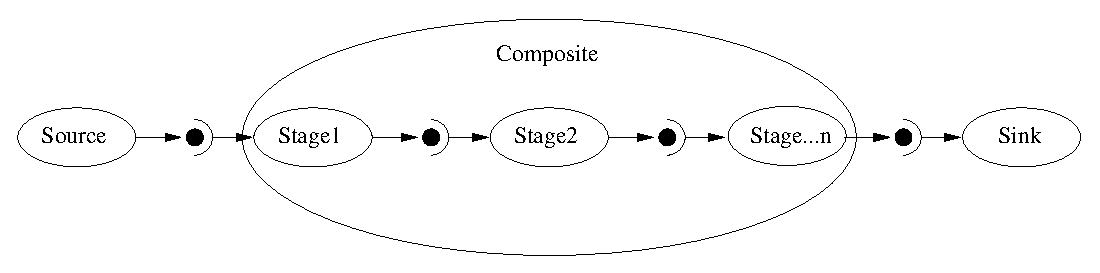
\includegraphics[width=0.9\textwidth]{CompositeFilterStages.eps}
  \itkcaption[Composite Filter Concept]{A Composite filter encapsulates a number of other filters.}
  \label{fig:CompositeFilterStages}
\end{figure}

\subsection{Implementing a Composite Filter}

There are a few considerations to take into account when implementing a
composite filter.  All the usual requirements for filters apply (as
discussed above), but the following guidelines should be considered:

\begin{enumerate}

\item The template arguments it takes must be sufficient to instantiate all of
the component filters.  Each component filter needs a type supplied by either
the implementor or the enclosing class.  For example, an
\code{ImageToImageFilter} normally takes an input and output image type (which
may be the same).  But if the output of the composite filter is a classified
image, we need to either decide on the output type inside the composite filter,
or restrict the choices of the user when she/he instantiates the filter.

\item The types of the component filters should be declared in the header,
  preferably with \code{protected} visibility.  This is because the
  internal structure normally should not be visible to users of the class,
  but should be to descendent classes that may need to modify or customize
  the behavior.

\item The component filters should be private data members of the composite
  class, as in \code{FilterType::Pointer}.

\item The default constructor should build the pipeline by creating the
  stages and connect them together, along with any default parameter
  settings, as appropriate.

\item The input and output of the composite filter need to be grafted on to
  the head and tail (respectively) of the component filters.

\end{enumerate}

This grafting process is illustrated in Figure~\ref{fig:CompositeExamplePipeline}.


\subsection{A Simple Example}

\begin{figure}
  \centering
  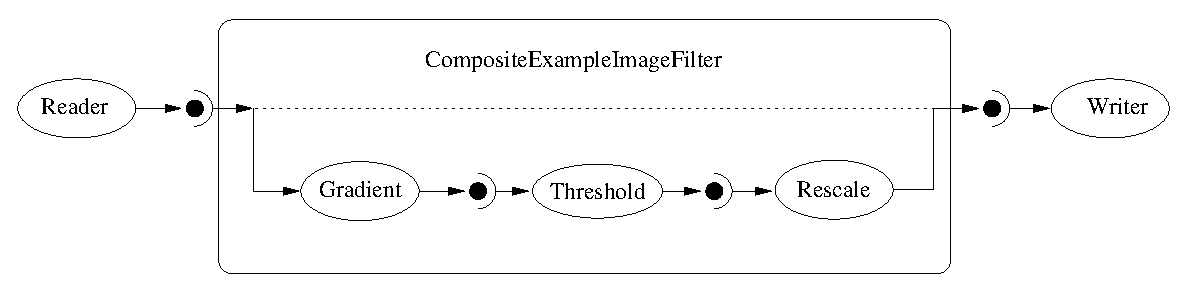
\includegraphics[width=0.9\textwidth]{CompositeExamplePipeline.eps}
  \itkcaption[Composite Filter Example]{Example of a typical composite filter. Note that the output of the last filter in the internal pipeline must be grafted into the output of the composite filter.}
  \label{fig:CompositeExamplePipeline}
\end{figure}

\input{CompositeFilterExample.tex}

%---------------------------------------------------------------------------

\fi


%
% TODO: include useful tips from mailing list as flagged
%

  \chapter{Software Process}
\label{chapter:SoftwareProcess}

An outstanding feature of ITK is the software process used to develop,
maintain and test the toolkit. The Insight Toolkit software continues to
evolve rapidly due to the efforts of developers and users located around the
world, so the software process is essential to maintaining its quality. If
you are planning to contribute to ITK, or use the Git source code repository,
you need to know something about this process (see
\ref{sec:ObtainingTheSoftware} on page \pageref{sec:ObtainingTheSoftware} to
learn more about obtaining ITK using Git). This information will help you
know when and how to update and work with the software as it changes. The
following sections describe key elements of the process.

\section{Git Source Code Repository}
\label{sec:GitRepository}

\index{ITK!Git repository}
\index{Git}

Git) is a tool for version control. It is a valuable resource for
software projects involving multiple developers.  The primary purpose
of Git is to keep track of changes to software. Git date and version
stamps every addition to files in the repository. Additionally, a user
may set a tag to mark a particular of the whole software. Thus, it is
possible to return to a particular state or point of time whenever
desired. The differences between any two points is represented by a
``diff'' file, that is a compact, incremental representation of
change. Git supports concurrent development so that two developers can
edit the same file at the same time, that are then (usually) merged
together without incident (and marked if there is a conflict). In
addition, branches off of the main development trunk provide parallel
development of software.

Developers and users can check out the software from the Git repository. When
developers introduce changes in the system,  Git facilitates to update the
local copies of other developers and users by downloading only the differences
between their local copy and the version on the repository.  This is an
important advantage for those who are interested in keeping up to date with the
leading edge of the toolkit. Bug fixes can be obtained in this way as soon as
they have been checked into the system.

ITK source code, data, and examples are maintained in a Git repository.  The
principal advantage of a system like Git is that it frees developers to try
new ideas and introduce changes without fear of losing a previous working
version of the software. It also provides a simple way to incrementally
update code as new features are added to the repository.

The ITK community use Git, and the Google web software tool Gerrit
(\url{http://review.source.kitware.com}) to facilitate a structured,
orderly method for developers to contribute new code and bug fixes to
ITK. The Gerrit review process allows anyone to submit a proposed
change to ITK, after which it will be reviewed by other developers
before being approved and merged into ITK.  For more information, see
\url{http://www.itk.org/Wiki/ITK/Git/Develop}.


\section{CDash Regression Testing System}
\label{sec:CDash}
\label{sec:QualityDashboard}

\index{Dashboard}
\index{Quality Dashboard}
\index{Dart}

One of the unique features of the ITK software process is its use of the CDash
regression testing system (\url{http://www.cdash.org}). In a
nutshell, what CDash does is to provide quantifiable feedback to developers as
they check in new code and make changes. The feedback consists of the results
of a variety of tests, and the results are posted on a publicly-accessible
Web page (to which we refer as a \emph{dashboard}) as shown in
Figure~\ref{fig:Dashboard}. The most recent dashboard is accessible from
\url{http://www.itk.org/ITK/resources/testing.html}). Since all users and developers of
ITK can view the Web page, the CDash dashboard serves as a vehicle for
developer communication, especially when new additions to the software is
found to be faulty.  The dashboard should be consulted before considering
updating software via Git.


\begin{figure}[ht]
\centering 
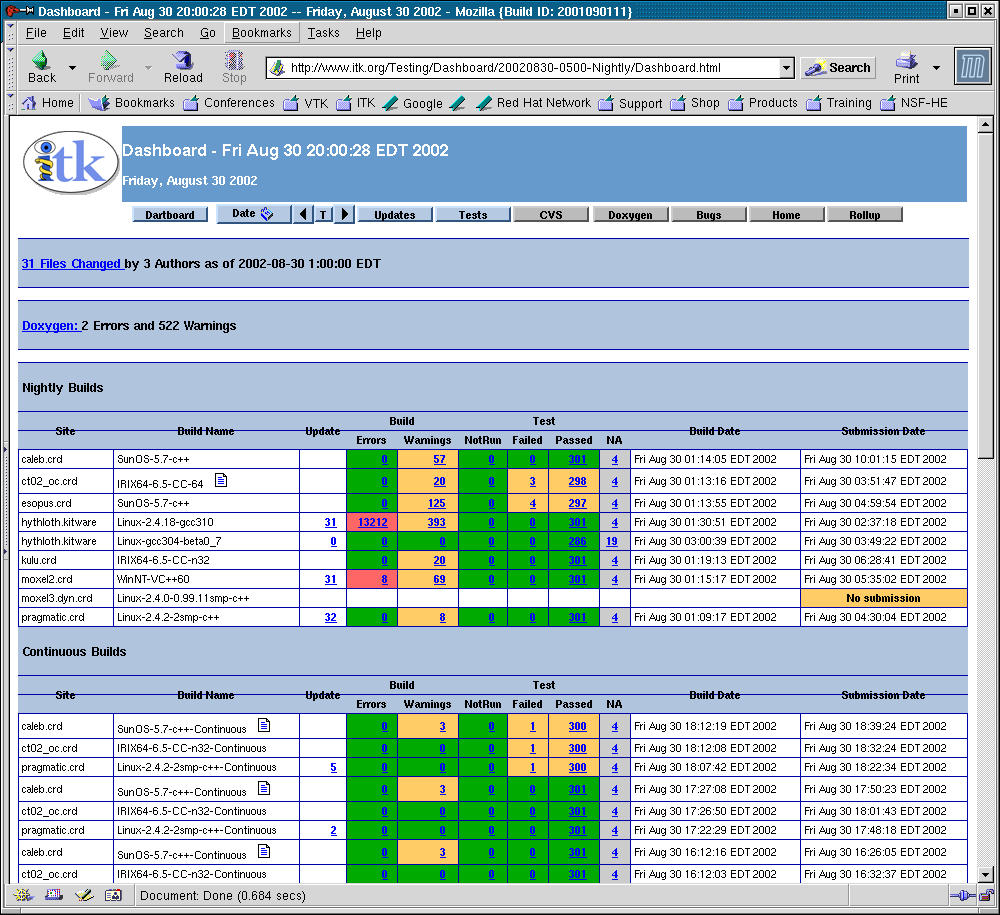
\includegraphics[width=0.7\textwidth]{Dashboard.eps}
\itkcaption[Dart Quality Dashboard]{On-line presentation of the quality
dashboard generated by CDash.}
\label{fig:Dashboard}
\end{figure}

Note that CDash is independent of ITK and can be used to manage quality
control for any software project. It is itself an open-source package and can
be obtained from

\begin{center} 
\url{http://public.kitware.com/Dart/HTML/Index.shtml}
\end{center} 

CDash supports a variety of test types. These include the following.
\begin{description}
        \item[Compilation.] All source and test code is compiled and linked. 
        Any resulting errors and warnings are reported on the dashboard.

        \item[Regression.] Some ITK tests produce images as output. Testing
        requires comparing each test's output against a valid baseline image. If
        the images match then the test passes. The comparison must be
        performed carefully since many 3D graphics systems (e.g., OpenGL)
        produce slightly different results on different platforms.

        \item[Memory.] Problems relating to memory such as leaks, uninitialized
        memory reads, and reads/ writes beyond allocated space can cause 
        unexpected results and program crashes. ITK checks run-time memory 
        access and management using Purify, a commercial package produced by 
        Rational. (Other memory checking programs will be added in the future.)

        \item[PrintSelf.] All classes in ITK are expected to print out all
        their instance variables (i.e., those with associated Set and Get 
        methods) correctly. This test checks to make sure
        that this is the case.

        \item[Unit.] Each class in ITK should have a corresponding unit test
        where the class functionalities are exercised and quantitatively
        compared against expected results. These tests are typically written
        by the class developer and should endeavor to cover all lines of code
        including \code{Set/Get} methods and error handling.

       \item[Coverage.] There is a saying among ITK developers: \emph{If it
        isn't covered, then it's broke.} What this means is that
        code that is not executed during testing is likely to be wrong. The
        coverage tests identify lines that are not executed in the
        Insight Toolkit test suite, reporting a total percentage
        covered at the end of the test. While it is nearly impossible to
        bring the coverage to 100\% because of error handling code and similar
        constructs that are rarely encountered in practice, the coverage
        numbers should be 75\% or higher. Code that is not covered well enough
        requires additional tests.
\end{description}

Figure~\ref{fig:Dashboard} shows the top-level dashboard web page. Each row
in the dashboard corresponds to a particular platform (hardware + operating
system + compiler). The data on the row indicates the number of compile
errors and warnings as well as the results of running hundreds of
small test programs. In this way the toolkit is tested both at compile time
and run time.

When a user or developer decides to update ITK source code from Git it is
important to first verify that the current dashboard is in good shape. This
can be rapidly judged by the general coloration of the dashboard. A green
state means that the software is building correctly and it is a good day to
start with ITK or to get an upgrade. A red state, on the other hand, is an
indication of instability on the system and hence users should refrain from
checking out or upgrading the source code.

Another nice feature of CDash is that it maintains a history of changes to the
source code (by coordinating with Git) and summarizes the changes as part of
the dashboard. This is useful for tracking problems and keeping up to date
with new additions to ITK.

\section{Working The Process}
\label{sec:WorkingTheProcess}

The ITK software process functions across three cycles---the continuous
cycle, the daily cycle, and the release cycle.

The continuous cycle revolves around the actions of developers as they check
code into Git. When changed or new code is checked into Git, the CDash
continuous testing process kicks in. A small number of tests are performed
(including compilation), and if something breaks, email is sent to all
developers who checked code in during the continuous cycle. Developers are
expected to fix the problem immediately.

The daily cycle occurs over a 24-hour period. Changes to the source base made
during the day are extensively tested by the nightly CDash regression testing
sequence. These tests occur on different combinations of computers and
operating systems located around the world, and the results are posted every
day to the CDash dashboard. Developers who checked in code are expected to
visit the dashboard and ensure their changes are acceptable---that is, they
do not introduce compilation errors or warnings, or break any other tests
including regression, memory, PrintSelf, and Set/Get. Again, developers are
expected to fix problems immediately.

The release cycle occurs a small number of times a year. This requires
tagging and branching the Git repository, updating documentation, and
producing new release packages. Although additional testing is performed to
insure the consistency of the package, keeping the daily Git build error free
minimizes the work required to cut a release.

ITK users typically work with releases, since they are the most
stable. Developers work with the Git repository, or sometimes with periodic
release snapshots, in order to take advantage of newly-added features. It is
extremely important that developers watch the dashboard carefully, and
\emph{update their software only when the dashboard is in good condition
(i.e., is ``green'')}. Failure to do so can cause significant disruption if a
particular day's software release is unstable.

\section{The Effectiveness of the Process}
\label{sec:Effectiveness}

The effectiveness of this process is profound. By providing immediate
feedback to developers through email and Web pages (e.g., the dashboard), the
quality of ITK is exceptionally high, especially considering the complexity
of the algorithms and system. Errors, when accidently introduced, are caught
quickly, as compared to catching them at the point of release. To wait to the
point of release is to wait too long, since the causal relationship between a
code change or addition and a bug is lost. The process is so powerful that it
routinely catches errors in vendor's graphics drivers (e.g., OpenGL drivers)
or changes to external subsystems such as the VXL/VNL numerics library. All
of these tools that make up the process (CMake, Git, and CDash) are
open-source. Many large and small systems such as VTK (The Visualization
Toolkit \url{http://www.vtk.org}) use the same process with similar
results. We encourage the adoption of the process in your environment.


\fi


\backmatter

%%%%%%%%%%%%%%%%%%%%%%%%%%%%%%%%%%%%%%%%%
%
%  Insert the bibliography using BibTeX
%
%%%%%%%%%%%%%%%%%%%%%%%%%%%%%%%%%%%%%%%%%

\bibliographystyle{plain}
\bibliography{\bibtexdatabasepath}


%%%%%%%%%%%%%%%%%%%%%%%%%%%%%%%%%%%%%%%%%
%
%  Insert the Index file
%
%%%%%%%%%%%%%%%%%%%%%%%%%%%%%%%%%%%%%%%%%

\InputIfFileExists{000-ITKSoftwareGuide-Book1.ind}


\begin{appendices}

\chapter{Licenses}

\section{Insight Toolkit License}
\label{sec:InsightToolkitLicense}
\verbatiminput{\ITKSOURCEDIR/LICENSE}


\section{Third Party Licenses}
The Insight Toolkit bundles a number of third party libraries that are used
internally.  The licenses of these libraries are as follows.

\subsection{DICOM Parser}
\verbatiminput{\ITKSOURCEDIR/Modules/ThirdParty/DICOMParser/src/DICOMParser/Copyright.txt}

\subsection{Double Conversion}
\verbatiminput{\ITKSOURCEDIR/Modules/ThirdParty/DoubleConversion/src/LICENSE}

\subsection{Expat}
\verbatiminput{\ITKSOURCEDIR/Modules/ThirdParty/Expat/src/expat/COPYING}

\subsection{GDCM}
\verbatiminput{\ITKSOURCEDIR/Modules/ThirdParty/GDCM/src/gdcm/Copyright.txt}

\subsection{GIFTI}
\verbatiminput{\ITKSOURCEDIR/Modules/ThirdParty/GIFTI/src/gifticlib/LICENSE.gifti}

\subsection{HDF5}
\verbatiminput{\ITKSOURCEDIR/Modules/ThirdParty/HDF5/src/itkhdf5/COPYING}

\subsection{JPEG}
% From its README.
\begin{verbatim}
The authors make NO WARRANTY or representation, either express or implied,
with respect to this software, its quality, accuracy, merchantability, or
fitness for a particular purpose.  This software is provided "AS IS", and you,
its user, assume the entire risk as to its quality and accuracy.

This software is copyright (C) 1991-2010, Thomas G. Lane, Guido Vollbeding.
All Rights Reserved except as specified below.

Permission is hereby granted to use, copy, modify, and distribute this
software (or portions thereof) for any purpose, without fee, subject to these
conditions:
(1) If any part of the source code for this software is distributed, then this
README file must be included, with this copyright and no-warranty notice
unaltered; and any additions, deletions, or changes to the original files
must be clearly indicated in accompanying documentation.
(2) If only executable code is distributed, then the accompanying
documentation must state that "this software is based in part on the work of
the Independent JPEG Group".
(3) Permission for use of this software is granted only if the user accepts
full responsibility for any undesirable consequences; the authors accept
NO LIABILITY for damages of any kind.

These conditions apply to any software derived from or based on the IJG code,
not just to the unmodified library.  If you use our work, you ought to
acknowledge us.

Permission is NOT granted for the use of any IJG author's name or company name
in advertising or publicity relating to this software or products derived from
it.  This software may be referred to only as "the Independent JPEG Group's
software".

We specifically permit and encourage the use of this software as the basis of
commercial products, provided that all warranty or liability claims are
assumed by the product vendor.


ansi2knr.c is included in this distribution by permission of L. Peter Deutsch,
sole proprietor of its copyright holder, Aladdin Enterprises of Menlo Park, CA.
ansi2knr.c is NOT covered by the above copyright and conditions, but instead
by the usual distribution terms of the Free Software Foundation; principally,
that you must include source code if you redistribute it.  (See the file
ansi2knr.c for full details.)  However, since ansi2knr.c is not needed as part
of any program generated from the IJG code, this does not limit you more than
the foregoing paragraphs do.

The Unix configuration script "configure" was produced with GNU Autoconf.
It is copyright by the Free Software Foundation but is freely distributable.
The same holds for its supporting scripts (config.guess, config.sub,
ltmain.sh).  Another support script, install-sh, is copyright by X Consortium
but is also freely distributable.

The IJG distribution formerly included code to read and write GIF files.
To avoid entanglement with the Unisys LZW patent, GIF reading support has
been removed altogether, and the GIF writer has been simplified to produce
"uncompressed GIFs".  This technique does not use the LZW algorithm; the
resulting GIF files are larger than usual, but are readable by all standard
GIF decoders.

We are required to state that
    "The Graphics Interchange Format(c) is the Copyright property of
    CompuServe Incorporated.  GIF(sm) is a Service Mark property of
    CompuServe Incorporated."
\end{verbatim}

\subsection{KWSys}
\verbatiminput{\ITKSOURCEDIR/Modules/ThirdParty/KWSys/src/KWSys/Copyright.txt}

\subsection{MetaIO}
\verbatiminput{\ITKSOURCEDIR/Modules/ThirdParty/MetaIO/src/MetaIO/License.txt}

\subsection{Netlib's SLATEC}
This code is in the public domain.  From
\url{http://www.netlib.org/slatec/guide}:
\begin{verbatim}
SECTION 4.  OBTAINING THE LIBRARY

The Library is in the public domain and distributed by the Energy Science
and Technology Software Center.

               Energy Science and Technology Software Center
               P.O. Box 1020
               Oak Ridge, TN  37831

               Telephone  615-576-2606
               E-mail  estsc%a1.adonis.mrouter@zeus.osti.gov
\end{verbatim}

\subsection{NIFTI}
\verbatiminput{\ITKSOURCEDIR/Modules/ThirdParty/NIFTI/src/nifti/LICENSE}

\subsection{NrrdIO}
\verbatiminput{\ITKSOURCEDIR/Modules/ThirdParty/NrrdIO/src/NrrdIO/000-README.txt}

\subsection{OpenJPEG}
\verbatiminput{\ITKSOURCEDIR/Modules/ThirdParty/OpenJPEG/src/LICENSE}

\subsection{PNG}
\verbatiminput{\ITKSOURCEDIR/Modules/ThirdParty/PNG/src/itkpng/libpng-LICENSE.txt}

\subsection{TIFF}
\verbatiminput{\ITKSOURCEDIR/Modules/ThirdParty/TIFF/src/itktiff/COPYRIGHT}

\subsection{VNL}
\verbatiminput{\ITKSOURCEDIR/Modules/ThirdParty/VNL/src/vxl/core/vxl_copyright.h}

\subsection{ZLIB}
% From its README.
\begin{verbatim}
 Acknowledgments:

   The deflate format used by zlib was defined by Phil Katz. The deflate
   and zlib specifications were written by L. Peter Deutsch. Thanks to all the
   people who reported problems and suggested various improvements in zlib;
   they are too numerous to cite here.

 Copyright notice:

  (C) 1995-2004 Jean-loup Gailly and Mark Adler

   This software is provided 'as-is', without any express or implied
   warranty.  In no event will the authors be held liable for any damages
   arising from the use of this software.

   Permission is granted to anyone to use this software for any purpose,
   including commercial applications, and to alter it and redistribute it
   freely, subject to the following restrictions:

   1. The origin of this software must not be misrepresented; you must not
      claim that you wrote the original software. If you use this software
      in a product, an acknowledgment in the product documentation would be
      appreciated but is not required.
   2. Altered source versions must be plainly marked as such, and must not be
      misrepresented as being the original software.
   3. This notice may not be removed or altered from any source distribution.

   Jean-loup Gailly        Mark Adler
   jloup@gzip.org          madler@alumni.caltech.edu

 If you use the zlib library in a product, we would appreciate *not*
 receiving lengthy legal documents to sign. The sources are provided
 for free but without warranty of any kind.  The library has been
 entirely written by Jean-loup Gailly and Mark Adler; it does not
 include third-party code.

 If you redistribute modified sources, we would appreciate that you include
 in the file ChangeLog history information documenting your changes. Please
 read the FAQ for more information on the distribution of modified source
 versions.
\end{verbatim}


\end{appendices}

%\ifitkPrintedVersion
%\cleardoublepage
%\newpage
\newpage
\thispagestyle{empty}
\includegraphics[width=14cm]{flyer-vtk-textbook.eps}
\newpage
\thispagestyle{empty}
\includegraphics[width=14cm]{flyer-cmake.eps}
\newpage
\thispagestyle{empty}
\includegraphics[width=14cm]{flyer-itk.eps}
\newpage
\thispagestyle{empty}
\includegraphics[width=14cm]{flyer-paraview.eps}
\newpage
\thispagestyle{empty}
\includegraphics[width=14cm]{flyer-activiz.eps}
\newpage
\thispagestyle{empty}
\includegraphics[width=14cm]{flyer-volview.eps}
\newpage
\thispagestyle{empty}
\includegraphics[width=14cm]{flyer-polyviz.eps}
\newpage
\thispagestyle{empty}
\includegraphics[width=14cm]{flyer-kitware.eps}

%\fi

%% Begin of comment out block
\iffalse
XXXXXXXXX
XXXXXXXXX
Garbage text
XXXXXXXXX
XXXXXXXXX
\fi
%% End of comment out block

\end{document}
